
\newcommand{\packagename}[2]{\texttt{PACKAGENAME packagename}---keyword and name of this instance of the {#1} Package. \texttt{packagename} must be provided as a string, with no more than 16 characters. If not provided, then this {#1} Package instance will be given the name {#2}\_ibcnum, where ibcnum is the sequential {#1} Package number as determined by the order in the GWF Name File.}

\newcommand{\auxname}[1]{\texttt{AUXILIARY auxname [auxname2 [auxname3] ...]}---defines a list of one or more auxiliary variables, with the names \texttt{auxname}, \texttt{auxname2}, and so forth.  There is no limit on the number of auxiliary variables that can be provided on this line; however, lists of information provided in subsequent blocks must have a column of data for each auxiliary variable defined here.   Comments cannot be provided anywhere on this line as they will be interpreted as auxiliary variable names.  Auxiliary variables may not be used by the {#1} model, but they will be available for use by other parts of the program.  The ``AUX'' keyword can be used as a substitute for ``AUXILIARY''. The program will terminate with an error if auxiliary variables are specified on more than one line in the options block.}  

\newcommand{\auxmultname}[1]{\texttt{AUXMULTNAME auxnamemult}---name of auxiliary variable to be used as multiplier of {#1}.}

\newcommand{\boundnames}[1]{\texttt{BOUNDNAMES}---keyword to indicate that boundary names may be provided with the list of {#1} cells.}

\newcommand{\boundnamesnotlayered}[1]{\texttt{BOUNDNAMES}---keyword to indicate that boundary names may be provided with the list of {#1} cells. Incompatible with the READASARRAYS option.}

%\newcommand{\layered}{\texttt{LAYERED}---keyword to indicate that input will be read as arrays. Invalid for an unstructured grid (DISU).}

\newcommand{\printinput}[1]{\texttt{PRINT\_INPUT}---keyword to indicate that the list of {#1} information will be written to the listing file immediately after it is read.}

\newcommand{\printflows}[1]{\texttt{PRINT\_FLOWS}---keyword to indicate that the list of {#1} flow rates will be printed to the listing file for every stress period in which ``BUDGET PRINT'' is specified in Output Control.  If there is no Output Control option and \texttt{PRINT\_FLOWS} is specified, then flow rates are printed for the last time step of each stress period.}

\newcommand{\saveflows}[1]{\texttt{SAVE\_FLOWS}---keyword to indicate that {#1} flow terms will be written to the file specified with ``BUDGET SAVE FILE'' in Output Control.}

\newcommand{\timeseries}[0]{\texttt{TIMESERIESFILE time-series-filename}---defines a time-series file defining time series that can be used to assign time-varying values. See the ``Time-Variable Input'' section for instructions on using the time-series capability.}

\newcommand{\timearrayseries}{\texttt{TIMEARRAYSERIESFILE time-array-series-filename}---defines a time-array-series file defining a time-array series that can be used to assign time-varying values. See the ��Time-Variable Input�� section for instructions on using the time-array series capability.}

\newcommand{\timearrayserieslayered}{\texttt{TIMEARRAYSERIESFILE time-array-series-filename}---name of a time-array-series file defining a time-array series that can be used to assign time-varying values when input is read in array form. See the ��Time-Variable Input�� section for instructions on using the time-array series capability. Valid only when the READASARRAYS option is used.}

\newcommand{\maxbound}[1]{\texttt{MAXBOUND maxbound}---keyword and integer value specifying the maximum number of {#1} cells that will be specified for use during any stress period.}

\newcommand{\iper}[1]{\texttt{BEGIN PERIOD iper}---keywords and integer value specifying the starting stress period number for which the following list of {#1} cells will apply.  The list of {#1} cells specified in this block will remain active with their specified head values until a new ``BEGIN PERIOD'' block is detected.}

\newcommand{\cellid}[0]{\texttt{cellid}---is the cell identifier, and depends on the type of grid that is used for the simulation.  For a structured grid that uses the DIS input file, \texttt{cellid} is the layer, row, and column.   For a grid that uses the DISV input file, \texttt{cellid} is the layer and cell2d number.  If the model uses the unstructured discretization (DISU) input file, then \texttt{cellid} is the node number for the cell.}

\newcommand{\xyzaux}[1]{\texttt{x,y,z}---represents the values of the auxiliary variables for each {#1}. The values of auxiliary variables must be present for each {#1}. The values must be specified in the order of the auxiliary variables specified in the OPTIONS block.  If the package supports time series and the Options block includes a TIMESERIESFILE entry (see the ``Time-Variable Input'' section), values can be obtained from a time series by entering the time-series name in place of a numeric value.}

\newcommand{\boundname}[1]{\texttt{boundname}---name of the {#1} cell.  \texttt{boundname} is an ASCII character variable that can contain as many as 40 characters.  If \texttt{boundname} contains spaces in it, then the entire name must be enclosed within single quotes.}

\newcommand{\newtonopt}[1]{\texttt{NEWTON}---keyword that activates the Newton-Raphson formulation for the {#1} Package.}

\newcommand{\obsopt}[1]{\texttt{OBS8 observation-input-filename}---keyword and name of input file to define observations for the {#1} package. See the ``Observation utility'' section for instructions for preparing observation input files. Table \ref{table:obstype} lists observation type(s) supported by the {#1} package.}

\newcommand{\mover}[1]{\texttt{MOVER}---keyword to indicate that this instance of the {#1} Package can be used with the Water Mover (MVR) Package.  When the \texttt{MOVER} option is specified, additional memory is allocated within the package to store the available, provided, and received water.}

\newcommand{\packageperioddescription}{All of the stress package information in the PERIOD block will continue to apply for subsequent stress periods until the end of the simulation, or until another PERIOD block is encountered.  When a new PERIOD block is encountered, all of the stresses from the previous block are replaced with the stresses in the new PERIOD block.  Note that this behavior is different from the advanced packages (MAW, SFR, LAK, and UZF).  To turn off all of the stresses for a stress period, a PERIOD block must be specified with no entries.  If a PERIOD block is not specified for the first stress period, then no stresses will be applied until the \texttt{iper} value of the first PERIOD block in the file.}

\newcommand{\packageperioddescriptionarray}[1]{All of the stress package information in the PERIOD block will continue to apply for subsequent stress periods until the end of the simulation, or until another PERIOD block is encountered.  When a new PERIOD block is encountered, the array-based input specified by the user will replace the arrays currently in memory.  If an array is not specified in the period block, then that array will retain its present values in memory.  With the array-based input, the user must specify a {#1} rate of zero in order to turn {#1} off for a stress period.  This behavior is different from list-based input in which an empty PERIOD block results in no stresses being applied.}

\newcommand{\advancedpackageperioddescription}[2]{All of the advanced stress package information in the PERIOD block will continue to apply for subsequent stress periods until the end of the simulation, or until another PERIOD block is encountered.  When a new PERIOD block is encountered only the {#2} specified in the new period block will be changed.  A {#1} not specified in the new period block will continue to behave according to its specification in the previous PERIOD block.  Note that this behavior is different from the simple stress packages (CHD, WEL, DRN, RIV, GHB, RCH and EVT), in which any stress not specified in a new PERIOD block will be removed.  To turn off all of the advanced stresses for a stress period, a PERIOD block must be specified with settings that deactivate the {#2}.  If a PERIOD block is not specified for the first stress period, then no stresses will be applied.}


%Introduction for input instructions
\SECTION{Introduction}
This document is a technical reference document that describes the motivation and implementation of functionality added to \mf since the initial release \citep{modflow6framework, modflow6gwf} and not documented in separate U.S. Geological Survey publications, for example \cite{modflow6xt3d}. Examples have been included for the \mf components summarized in table~\ref{table:mf6enhance}.

\begin{table}[!ht]
  \small
  \centering
  \caption{\mf enhancements} \tabularnewline 

  \begin{tabular}{z{3.50cm}
                  z{3.50cm}
                  z{3.50cm}
                  z{3.50cm}
                  }
    % header
    \hline
    \rowcolor{Gray}
    \multicolumn{1}{ z{3.50cm} }{\textbf{\mf enhancements}} & 
    \multicolumn{1}{ z{3.50cm} }{\textbf{Chapter}} & 
    \multicolumn{1}{ z{3.50cm} }{\textbf{Initial \mf version}} & 
    \multicolumn{1}{ z{3.50cm} }{\textbf{Latest update -- \mf version}} \\
    \hline

    Specific Discharge &  \ref{ch:spdis} & 6.0.2    &  6.1.0  \\
\rowcolor{Gray}
    DRN Package Discharge Scaling &  \ref{ch:drn} & 6.1.1    &  --   \\
    MAW Package Connection Flow Correction &  \ref{ch:maw-qcorr} & 6.1.1    &  --   \\
\rowcolor{Gray}
    STO Package Specific Storage Revision &  \ref{ch:sto-mod} & 6.1.3    &  --   \\
    TVK and TVS Capabilities for NPF & \ref{ch:tvk-tvs} & 6.3.0  &  -- \\
    \hline
  \end{tabular}
  \label{table:mf6enhance}
\end{table}




%Instructions for running a simulation
\SECTION{Running a Simulation}
\input{running_simulation.tex}

%General form of input instructions
\SECTION{Form of Input Instructions}
\mf differs from its predecessors in the form of the input.  Whereas previous MODFLOW versions read numerical values, arrays, and lists in a highly structured form, \mf reads information in the form of blocks and keywords.  \mf also reads arrays and lists of information, but these arrays and lists are tagged with identifying block names or keywords.  \mf will terminate with an error if it detects an unrecognized block or keyword.

\subsection{Block and Keyword Input} 

Input to \mf is provided within blocks.  A block is a section of an ASCII input file that begins with a line that has ``BEGIN'' followed by the name of the block and ends with a line the begins with ``END'' followed by the name of the block.  \mf will terminate with an error if blocks do not begin and end with the same name, or if a ``BEGIN'' or ``END'' line is missing.  Information within a block differs depending on the part of \mf that reads the block.  In general, keywords are used within blocks to turn options on or specify the type of information that follows the keyword.  If an unrecognized keyword is encountered in a block, \mf will terminate with an error.

The keyword approach is adopted in \mf to improve readability of the \mf input files, enhance discovery of errors in input files, and improve support for backward compatibility by allowing the program to expand in functionality while allowing previously developed models to be run with newer versions of the program.

Within these user instructions, keywords are shown in capital letters to differentiate them from other input that is provided by the user.  For example, ``BEGIN'' and ``END'' are recognized by \mf, and so they are capitalized.  Also, line indentation is used within these user instructions to help with readability of the blocks.  Typically, lines within a block are indented two spaces to accentuate that the lines are part of the block.  This indentation is not enforced by the program, but users are encouraged to use it within their own input files to improve readability.

Unless stated otherwise in this user guide, information contained within a block can be listed in any order.  If the same keyword is provided more than once, then the program will use the last information provided by that keyword.

Comment lines and blanks lines are also allowed within most blocks and within most input files.  Valid comment characters include ``\#'' ``!'', and ``//''.  Comments can also be placed at the end of some input lines, after the required information.  Comments are not allowed at the end of some lines if the program is required to read an arbitrary number of non-keyword items.  Comments included at the end of the line must be separated from the rest of the line by at least one space.

Unless otherwise noted in the input instructions, multiple blocks of the same name cannot be specified in a single input file.  The block order within the input file must follow the order presented in the input instructions.  Each input file typically begins with an OPTIONS block, which is generally not required, followed by one or more data blocks.

The following is an example of how the input instructions for a block are presented in this document.  
\begin{lstlisting}[style=blockdefinition]
BEGIN OPTIONS
  [AUXILIARY <auxiliary(naux)>]
  [PRINT_INPUT]
  [MAXIMUM_ITERATION <maxsfrit>]
END OPTIONS
\end{lstlisting}
This example shows the items that may be specified with this OPTIONS block.  Optional items are enclosed between ``['' and ``]'' symbols.  The ``\texttt{<}'' and ``\texttt{>}'' symbols indicate a variable that must be provided by the user.  In this case, \texttt{auxiliary} is an array of size \texttt{naux}.  Because there are bracket symbols around the entire item, the user it not required to specify anything for this item.  Likewise, the user may or may not invoke the ``\texttt{PRINT\_INPUT}'' option.  Lastly, the user can specify ``\texttt{MAXIMUM\_ITERATION}'' followed by a numeric value for ``\texttt{maxsfrit}''.  If the user does not specify an optional item, then a default condition will apply.  Behavior of the default condition is described in the input instructions for that item.

\vspace{6pt}\noindent A valid user input block for OPTIONS might be:

\begin{lstlisting}[style=inputfile]
#This is my options block
BEGIN OPTIONS
  AUXILIARY temperature salinity
  MAXIMUM_ITERATION 10
END OPTIONS
\end{lstlisting}

\noindent The following is another valid user input block for OPTIONS:

\begin{lstlisting}[style=inputfile]
#This is an alternative options block
BEGIN OPTIONS
  # Assign two auxiliary variables
  AUXILIARY temperature salinity
  # Specify the maximum iteration
  MAXIMUM_ITERATION 10
  #specify the print input option
  PRINT_INPUT
END OPTIONS
#done with the options block
\end{lstlisting}

\subsection{Specification of Block Information in OPEN/CLOSE File} 
For most blocks, information can be read from a separate text file.  In this case, all of the information for the block must reside in the text file.  The file name is specified using the OPEN/CLOSE keyword as the first and only entry in the block as follows:

\begin{lstlisting}[style=inputfile]
#This is an alternative options block
BEGIN OPTIONS
  OPEN/CLOSE myoptblock.txt
END OPTIONS
\end{lstlisting}

\noindent When MODFLOW encounters the OPEN/CLOSE keyword, the program opens the specified file on unit 99 and continues processing the information in the file as if it were within the block itself.  When the program reaches the end of the file, the file is closed, and the program returns to reading the original package file.  The next line after the OPEN/CLOSE line must end the block.

Some blocks do not support the OPEN/CLOSE capability.  A list of all of the blocks, organized by component and input file type, are listed in a table in appendix A.  This table also indicates the blocks that do not support the OPEN/CLOSE capability.

\subsection{File Name Input}
Some blocks may require that a file name be entered.  Although spaces within a file name are not generally recommended, they can be specified if the entire file name is enclosed within single quotes, which means that the file name itself cannot have a single quote within it.  On Windows computers, file names are not case sensitive, and thus, ``model.dis'' can be referenced within the input files as ``MODEL.DIS''.  On some other operating systems, however, file names are case sensitive and the case used in the input instructions must exactly reflect the case used to name the file.

\subsection{Lengths of Character Variables}
Character variables, which are used to store names of models, packages, observations and other objects, are limited in the number of characters that can be used. Table \ref{table:characterlength} lists the limit used for each type of character variable.

\FloatBarrier
\begin{table}[H]
\caption{Character variable maximum sizes}
\small
\begin{center}
\begin{tabular*}{\columnwidth}{l l l}
\hline
\hline
\textbf{Size limit name} & \textbf{Size} & \textbf{Variable(s) affected} \\
\hline
LENAUXNAME & 16 & Auxiliary variable names \\
LENBOUNDNAME & 40 & Boundary names \\
LENMODELNAME & 16 & Model names \\
LENOBSNAME & 40 & Observation names \\
LENPACKAGENAME & 16 & Package names \\
LENSOLUTIONNAME & 16 & Solution names \\
LENTIMESERIESNAME & 40 & Time-series and time-array-series names \\
\hline
\end{tabular*}
\label{table:characterlength}
\end{center}
\normalsize
\end{table}

\FloatBarrier

\subsection{Integer and Floating Point Variables}
\mf uses integer and floating point variables throughout the program.  The sizes of these variables are defined in a single module within the program.  Information about the precision, range, and size of integers and floating point real variables is written to the top of the simulation list file: 

{\small
\begin{lstlisting}[style=modeloutput]
MODFLOW was compiled using uniform precision.

Real Variables
  KIND: 8
  TINY (smallest non-zero value):    2.225074-308
  HUGE (largest value):    1.797693+308
  PRECISION: 15
  SIZE IN BITS: 64

Integer Variables
  KIND: 4
  HUGE (largest value): 2147483647
  SIZE IN BITS: 32

Long Integer Variables
  KIND: 8
  HUGE (largest value): 9223372036854775807
  SIZE IN BITS: 64

Logical Variables
  KIND: 4
  SIZE IN BITS: 32
\end{lstlisting}
}

This information indicates that real variables have about 15 digits of precision.  The smallest positive non-zero value that can be stored is 2.2e-308.  The largest value that can be stored is 1.8e+308.  If the user enters a value in an input file that cannot be stored, such as 1.9335e-310 for example, then the program can produce unexpected results.  This does not affect an exact value of zero, which can be stored accurately.  Integer variables also have a maximum and minimum value, which is about 2 billion.  Values larger and smaller than this cannot be stored.  These numbers are rarely exceeded for most practical problems, but as the size of models (number of nodes) increase into the billions, then the program may need to be recompiled using a larger size for integer variables. Long integers are used to calculate the amount of memory allocated in the memory manager:

{\small
\begin{lstlisting}[style=modeloutput]
 MEMORY MANAGER TOTAL STORAGE BY DATA TYPE, IN MEGABYTES
 -------------------------------
                    ALLOCATED   
 DATA TYPE           MEMORY     
 -------------------------------
 Character        1.53300000E-03
 Logical          4.40000000E-05
 Integer          100.03799     
 Real             223.43994     
 -------------------------------
 Total            323.47951     
 -------------------------------
\end{lstlisting}
}

Currently, standard precision 4 byte logical variables are used throughout the program.

\subsection{Array Input (READARRAY)}
Some \mf Model packages require arrays of information to be provided by the user.  This information is read using a generic READARRAY capability in \mf.  Within this user guide, variables that are read with READARRAY are marked accordingly, as shown in example input instructions for a DATA block.  

\begin{lstlisting}[style=blockdefinition]
BEGIN DATA
  ARRAY1
    <array1(nval)> -- READARRAY
END DATA
\end{lstlisting}

\noindent In this example, the uppercase ARRAY1 is a text string that is recognized by the program.  While reading through the DATA block, the program would recognize ARRAY1, and would then use READARRAY to fill \texttt{array1} with \texttt{nval} values.

\subsubsection{READARRAY Control Line}

READARRAY works similar to the array readers in previous MODFLOW versions.  It begins by reading a control line.  The control line has one of three forms shown below, and is limited to a length of 999 characters.

\begin{lstlisting}[style=blockdefinition]
1. CONSTANT <constant> 
\end{lstlisting}
With CONSTANT, all values in the array are set equal to \texttt{constant}. 

\begin{lstlisting}[style=blockdefinition]
2. INTERNAL [FACTOR <factor>] [IPRN <iprn>] 
\end{lstlisting}
With INTERNAL, the individual array elements will be read from the same file that contains the control line. 

\begin{lstlisting}[style=blockdefinition]
3. OPEN/CLOSE <fname> [FACTOR <factor>] [(BINARY)] [IPRN <iprn>]
\end{lstlisting}
With OPEN/CLOSE, the array will be read from the file whose name is specified by \texttt{fname}. This file will be opened just prior to reading the array and closed immediately after the array is read. A file that is read using this control line can contain only a single array. 

\subsubsection{READARRAY Variable Descriptions}

\begin{description}

\item \texttt{<constant>}---is a real number constant for real arrays and an integer constant for integer arrays. The \texttt{constant} value is assigned to the entire array. 

\item \texttt{FACTOR <factor>}---are a keyword and a real number factor for real arrays and an integer factor for integer arrays. The individual elements of the array are multiplied by \texttt{factor} after they are read. If \texttt{factor} is specified as 0, then it is changed to 1.

\item \texttt{(BINARY)}---is an option that indicates the OPEN/CLOSE file contains array data in binary (unformatted) form. A binary file that can be read by MODFLOW may be created in only two ways. The first way is to use MODFLOW to create the file by saving heads in a binary file. This is commonly done when the user desires to use computed heads from one simulation as initial heads for a subsequent simulation. The other way to create a binary file is to write a special program that generates a binary file.  ``(BINARY)'' can be specified only when the control line is OPEN/CLOSE.

\item \texttt{IPRN <iprn>}---are a keyword and a flag that indicates whether the array being read should be written to the Listing File after the array has been read and a code for indicating the format that should be used when the array is written. The format codes are the same as for MODFLOW-2005. IPRN is set to zero when the specified value exceeds those defined. If IPRN is less than zero or if the keyword and flag are omitted, the array will not be printed.  This IPRN capability is not functional for all data sets, and will eventually become unsupported for all packages.  For some packages that have transitioned to the new input data processor, the EXPORT\_ARRAY\_ASCII option can be specified in the package OPTIONS block.  When this option is active, input arrays will be written to external text files.

\end{description}

\begin{longtable}{p{2cm} p{2cm} p{2cm} p{2cm}}
\caption{IPRN Code and corresponding print formats for array readers.  These print codes determine how the user-provided array is written to the list file} 
\tabularnewline
\hline
\hline
\textbf{IPRN} & \textbf{Real} & \textbf{Integer} \\
\hline
\endhead
\hline
\endfoot
0 & 10G11.4 & 10I11 \\
1 & 11G10.3 & 60I1 \\
2 & 9G13.6 & 40I2 \\
3 & 15F7.1 & 30I3 \\
4 & 15F7.2 & 25I4 \\
5 & 15F7.3 & 20I5 \\
6 & 15F7.4 & 10I11 \\
7 & 20F5.0 & 25I2 \\
8 & 20F5.1 & 15I4 \\
9 & 20F5.2 & 10I6 \\
10 & 20F5.3 &  \\
11 & 20F5.4 &  \\
12 & 10G11.4 & \\
13 & 10F6.0 &  \\
14 & 10F6.1 &  \\
15 & 10F6.2 &  \\
16 & 10F6.3 &  \\
17 & 10F6.4 &  \\
18 & 10F6.5 &  \\
19 & 5G12.5 &  \\
20 & 6G11.4 &  \\
21 & 7G9.2 &  \\
%\label{table:ndim}
\end{longtable}


\subsubsection{READARRAY Examples}

The following examples use free-format control lines for reading an array. The example array is a real array consisting of 4 rows with 7 columns per row: 

\begin{lstlisting}[style=inputfile]
CONSTANT 5.7      This sets an entire array to the value "5.7". 
INTERNAL FACTOR 1.0 IPRN 3            This reads the array values from the 
 1.2 3.7 9.3 4.2 2.2 9.9 1.0      file that contains the control line. 
 3.3 4.9 7.3 7.5 8.2 8.7 6.6      Thus, the values immediately follow the 
 4.5 5.7 2.2 1.1 1.7 6.7 6.9      control line. 
 7.4 3.5 7.8 8.5 7.4 6.8 8.8 
OPEN/CLOSE inp.txt FACTOR 1.0 IPRN 3    Read array from formatted file "inp.dat". 
OPEN/CLOSE inp.bin FACTOR 1.0 (BINARY) IPRN 3     Read array from binary file "inp.bin". 
OPEN/CLOSE test.dat FACTOR 1.0 IPRN 3     Read array from file "test.dat". 
\end{lstlisting}


Some arrays define information that is required for the entire model grid, or part of a model grid.  This type of information is provided in a special type of data block called a ``GRIDDATA'' block.  For example, hydraulic conductivity is required for every cell in the model grid.  Hydraulic conductivity is read from a ``GRIDDATA'' block in the \mf GWF NPF Package input file.  For GRIDDATA arrays with one value for every cell in the model grid, the arrays can optionally be read in a LAYERED format, in which an array is provided for each layer of the grid.  Alternatively, the array can be read for the entire model grid.  As an example, consider the GRIDDATA block for the \mf GWF or GWT IC Package shown below:

\lstinputlisting[style=blockdefinition]{./mf6ivar/tex/gwf-ic-griddata.dat}

Here, the initial heads for the model are provided in the \texttt{strt} array.  If the optional LAYERED keyword is present, then a separate array is provided for each layer.  If the LAYERED keyword is not present, then the entire starting head array is read at once.  The LAYERED keyword may be useful to discretization packages of type DIS and DISV, which support the concept of layers.  Models defined with the DISU Package are not layered.

For a structured DIS model, the READARRAY utility is used to read arrays that are dimensioned to the full size of the grid (of size \texttt{nlay*nrow*ncol}). This utility first reads an array name, which associates the input to be read with the desired array.  For these arrays, an optional keyword ``LAYERED'' can be located next to the array name.  If ``LAYERED'' is detected, then a control line is provided for each layer and the array is filled with values for each model layer.  If the ``LAYERED'' keyword is absent, then a single control line is used and the entire array is filled at once.

For example, the following block shows one way the \mf GWF model starting head array (STRT) could be specified for a model with 4 layers.  Following the array name and the ``LAYERED'' keyword are four control lines, one for each layer.

\begin{lstlisting}[style=inputfile]
  STRT LAYERED
     CONSTANT 10.0  #layer 1
     CONSTANT 10.0  #layer 2
     CONSTANT 10.0  #layer 3
     CONSTANT 10.0  #layer 4
\end{lstlisting}

In this next example, the ``LAYERED'' keyword is absent.  In this case, the control line applies to the entire \texttt{strt} array.  One control line is required, and a constant value of 10.0 will be assigned to STRT for all cells in the model grid.

\begin{lstlisting}[style=inputfile]
  STRT
     CONSTANT 10.0  #applies to all cells in the grid
\end{lstlisting}

In the next example, the ``LAYERED'' keyword is present and binary files are used for each layer. A control line with the ``BINARY'' keyword is required for each layer.

\begin{lstlisting}[style=inputfile]
  STRT LAYERED
     OPEN/CLOSE strt.layer1.bin (BINARY)  #layer1
     OPEN/CLOSE strt.layer2.bin (BINARY)  #layer2
     OPEN/CLOSE strt.layer3.bin (BINARY)  #layer3
     OPEN/CLOSE strt.layer4.bin (BINARY)  #layer4
\end{lstlisting}

In the next example, the ``LAYERED'' keyword is absent. In this case, a single control line with the ``BINARY'' keyword is required and the binary file will include the entire data array.

\begin{lstlisting}[style=inputfile]
  STRT
     OPEN/CLOSE strt.bin (BINARY)  #layers1-4
\end{lstlisting}

A consequence of the way binary input files have been implemented in \mf, simulated dependent variable binary output (for example, head and concentration) cannot be used as binary array input for a model. Instead, simulated dependent variable binary output must be processed and split into separate binary files for each layer or combined into a single array equal to the size of the grid (for DIS grids this would be an array equal to NCOL * NROW * NLAY).

\subsubsection{Description of Binary Array Input Files}
All floating point variables are written to the binary input files as DOUBLE PRECISION Fortran variables. Integer variables are written to the input files as Fortran integer variables. Some variables are character strings and are indicated as so in the following descriptions. Binary array data are written using the following two records:

\vspace{5mm}
\noindent Record 1: \texttt{KSTP,KPER,PERTIM,TOTIM,TEXT,M1,M2,M3} \\
\noindent Record 2: \texttt{DATA} \\

\vspace{5mm}
\noindent where

\begin{description} \itemsep0pt \parskip0pt \parsep0pt
\item \texttt{KSTP} is the time step number;
\item \texttt{KPER} is the stress period number;
\item \texttt{PERTIM} is the time value for the current stress period; 
\item \texttt{TOTIM} is the total simulation time;
\item \texttt{TEXT} is a character string (character*16);
\item \texttt{M1} is the length of the data in the fastest varying direction;
\item \texttt{M2} is the length of the data in the second fastest varying direction;
\item \texttt{M3} can be any value but is typically 1 or the layer number for the data; and
\item \texttt{DATA} is the array data of size (M1*M2).
\end{description}
 
\noindent The values specified for \texttt{M1}, \texttt{M2}, and \texttt{M3} in Record 1 are dependent on the grid type and if the ``LAYERED'' keyword is present on the READARRAY control line.  For binary array data, \texttt{KSTP}, \texttt{KPER}, \texttt{PERTIM}, \texttt{TOTIM}, and \texttt{TEXT} can be set to any value. Binary array input file specifications for each discretization type are given below.

\paragraph{DIS Grids}
For DIS grids,  \texttt{M1=NCOL}, \texttt{M2=NROW}, and \texttt{M3=ILAY} when the ``LAYERED'' keyword is present on the READARRAY control line. For this case, record 1 and 2 should be written as:

\vspace{5mm}
\noindent Record 1: \texttt{KSTP,KPER,PERTIM,TOTIM,TEXT,M1,M2,M3} \\
\noindent Record 2: \texttt{((DATA(J,I,ILAY),J=1,NCOL),I=1,NROW)} \\

\vspace{5mm}
\noindent where

\begin{description} \itemsep0pt \parskip0pt \parsep0pt
\item \texttt{NCOL} is the number of columns;
\item \texttt{NROW} is the number of rows; and
\item \texttt{ILAY} is the layer number.
\end{description}

\noindent For DIS grids, \texttt{M1=NCOL*NROW*NLAY}, \texttt{M2=1}, and \texttt{M3=1} when the ``LAYERED'' keyword is absent on the READARRAY control line. For this case, record 1 and 2 should be written as:

\vspace{5mm}
\noindent Record 1: \texttt{KSTP,KPER,PERTIM,TOTIM,TEXT,M1,M2,M3} \\
\noindent Record 2: \texttt{(((DATA(J,I,K),J=1,NCOL),I=1,NROW),K=1,NLAY)} \\

\vspace{5mm}
\noindent where

\begin{description} \itemsep0pt \parskip0pt \parsep0pt
\item \texttt{NLAY} is the number of layers.
\end{description}

\paragraph{DISV Grids}
For DISV grids, \texttt{M1=NCPL}, \texttt{M2=1}, and \texttt{M3=ILAY} when the ``LAYERED'' keyword is present on the READARRAY control line. For this case, record 1 and 2 should be written as:

\vspace{5mm}
\noindent Record 1: \texttt{KSTP,KPER,PERTIM,TOTIM,TEXT,M1,M2,M3} \\
\noindent Record 2: \texttt{(DATA(J,ILAY),J=1,NCPL)} \\

\vspace{5mm}
\noindent where

\begin{description} \itemsep0pt \parskip0pt \parsep0pt
\item \texttt{NCPL} is the number of cells per layer.
\end{description}

\noindent For DISV grids, \texttt{M1=NCPL*NLAY}, \texttt{M2=1}, and \texttt{M3=1} when the ``LAYERED'' keyword is absent on the READARRAY control line. For this case, record 1 and 2 should be written as:

\vspace{5mm}
\noindent Record 1: \texttt{KSTP,KPER,PERTIM,TOTIM,TEXT,M1,M2,M3} \\
\noindent Record 2: \texttt{((DATA(J,K),J=1,NCPL),K=1,NLAY)} \\


\paragraph{DISU Grids}
For DISU grids, \texttt{M1=NODES}, \texttt{M2=1}, \texttt{M3=1}. For this case, record 1 and 2 should be written as:


\vspace{5mm}
\noindent Record 1: \texttt{KSTP,KPER,PERTIM,TOTIM,TEXT,M1,M2,M3} \\
\noindent Record 2: \texttt{(DATA(N),N=1,NODES)} \\

\vspace{5mm}
\noindent where

\begin{description} \itemsep0pt \parskip0pt \parsep0pt
\item \texttt{NODES} is the number cells in the model grid.
\end{description}

\subsection{List Input}
Some items consist of several variables, such as layer, row, column, stage, and conductance, for example.  List input refers to a block of data with a separate item on each line.  For some common list types, the first set of variables is a cell identifier (denoted as \texttt{cellid} in this guide), such as layer, row, and column. With lists, the input data for each item must start on a new line. All variables for an item are assumed to be contained in a single line.  Each input variable has a data type, which can be Double Precision, Integer, or Character. Integers are whole numbers and must not include a decimal point or exponent. Double Precision numbers can include a decimal point and an exponent. If no decimal point is included in the entered value, then the decimal point is assumed to be at the right side of the value. Any printable character is allowed for character variables. 

Variables starting with the letters I-N are most commonly integers; however, in some instances, a character string may start with the letters I-N. Variables starting with the letters A-H and O-Z are primarily double precision numbers; however, these variable names may also be used for character data.  In \mf all variables are explicitly declared within the source code, as opposed to the implicit type declaration in previous MODFLOW versions.  This explicit declaration means that the variable type can be easily determined from the source code.

Free formatting is used throughout the input instructions.  With free format, values are not required to occupy a fixed number of columns in a line. Each value can occupy one or more columns as required to represent the value; however, the values must still be included in the prescribed order. One or more spaces, or a single comma optionally combined with spaces, must separate adjacent values. Also, a numeric value of zero must be explicitly represented with 0 and not by one or more spaces when free format is used, because detecting the difference between a space that represents 0 and a space that represents a value separator is not possible. Free format is similar to Fortran's list directed input.

Two capabilities included in Fortran's list-directed input are not included in the free-format input implemented in \mf. Null values in which input values are left unchanged from their previous values are not allowed. In general, MODFLOW's input values are not defined prior to their input.  A ``/'' cannot be used to terminate an input line without including values for all the variables; data values for all required input variables must be explicitly specified on an input line.  For character data, MODFLOW's free format implementation is less stringent than the list-directed input of Fortran. Fortran requires character data to be delineated by apostrophes. MODFLOW does not require apostrophes unless a blank or a comma is part of a character variable.

As an example of a list, consider the PERIOD block for the GHB Package.  The input format is  shown below:

\lstinputlisting[style=blockdefinition]{./mf6ivar/tex/gwf-ghb-period.dat}

Each line represents a separate item, which consists of variables.  In this case, the first variable of the item, \texttt{cellid} is an array of size \texttt{ncelldim}.  The next two variables of the item are \texttt{bhead} and \texttt{cond}.  Lastly, the item has two optional variables, \texttt{aux} and \texttt{boundname}.  Three of the variables shown in the list are colored in blue.  Variables that are colored in blue mean that they can be represented with a time series.  The time series capability is described in the section on Time-Variable Input in this document.  

The following is simple example of a PERIOD block for the GHB Package, which shows how a list is entered by the user.

\begin{lstlisting}[style=inputfile]
BEGIN PERIOD 1
#      lay       row       col     stage      cond
         1        13         1     988.0     0.038
         1        14         9    1045.0     0.038
END PERIOD
\end{lstlisting}

As described earlier in the section on ``Block and Keyword Input,'' block information can be read from a separate text file.  To activate reading a list from separate text file, the first and only entry in the block must be a control line of the following form:  

\begin{lstlisting}[style=blockdefinition]
  OPEN/CLOSE <fname>
\end{lstlisting}

\noindent where \texttt{fname} is the name of the file containing the list.  Lists for the stress packages (CHD, WEL, DRN, RIV, GHB, RCH, and EVT) have an additional BINARY option.  The BINARY  option is not supported for the advanced stress packages (LAK, MAW, SFR, UZF, LKT, MWT, SFT, UZT).  The BINARY options is specified as follows:

\begin{lstlisting}[style=blockdefinition]
  OPEN/CLOSE <fname> [(BINARY)]
\end{lstlisting}

If the (BINARY) keyword is found on the control line, then the file is opened as an unformatted file on unit 99, and the list is read.  There are a number of requirements for using the (BINARY) option for lists.  All stress package lists begin with integer values for the \texttt{cellid} (layer, row, and column, for example).  These values must be represented as integer numbers in the unformatted file.  Also, all auxiliary data must be included in the binary file; auxiliary data must be represented as double precision numbers.  Lastly, the (BINARY) option does not support entry of \texttt{boundname}, and so the BOUNDNAMES option should not be activated in the OPTIONS block for the package.  
\subsubsection{Description of Binary List Input Files}
All floating point variables are written to the binary input files as DOUBLE PRECISION Fortran variables. Integer variables are written to the input files as Fortran integer variables. Auxiliary variables can be included in binary list input files but as indicated previously binary list input files can not be used for packages that include BOUNDNAMES keyword in the OPTIONS block. The format of binary list data are described below.

\vspace{5mm}
\noindent Record 1: \texttt{(CELLID(N),(RLIST(I,N),I=1,NDAT)(AUXVAR(I,N),I=1, NAUX), N=1,NLIST)}\\

\noindent where

\begin{description} \itemsep0pt \parskip0pt \parsep0pt
\item \texttt{CELLID} is the cell identifier, and depends on the type of grid that is used for the simulation.;
\item \texttt{RLIST} is a double precision two-dimensional array of size (NDAT,NLIST) containing the stress package PERIOD data;
\item \texttt{NDAT} is the number of columns in RLIST, which is the number of columns of real data in the stress package PERIOD data;
\item \texttt{AUXVAR} is a double precision two-dimensional array of size (NAUX,NLIST)  containing the auxilary data for the stress package PERIOD data;
\item \texttt{NAUX} is the number of columns in AUXVAR, which is the number of columns of real auxiliary data the in stress package PERIOD data;
\item \texttt{NLIST} is the size of the list;
\end{description}

\noindent For a structured grid that uses the DIS input file, CELLID is the layer, row, and column. For a grid that uses the DISV input file, CELLID is the layer and CELL2D number. If the model uses the unstructured discretization (DISU) input file, CELLID is the node number for the cell. \texttt{NLIST} must be less than or equal to \texttt{MAXBOUND} for a stress package. \texttt{NAUX} is determined by the number of \texttt{AUXILIARY} variable names define in the OPTIONS block for the stress package.


%Processing of program input
\SECTION{Processing of Program Input}
An effort is underway to process program input early in program runtime, before the simulation is created, in a general way that is not dependent on any given component.  This capability is called the \mf Input Data Processor (IDP).  Components that have been updated to use IDP no longer directly read or process file inputs but instead access input data from internally managed memory locations. 

\subsection{Supported Components}

A specific set of \mf components has been updated in the current version to use the IDP routines, as shown in Table~\ref{table:idmsupported}.  Two integration steps have been taken for each file type listed in the table.  First, IDP has been updated to support the reading and loading of variable input data for the component.  File types listed in the table, each previously read and processed by the component, are now processed by IDP.  Second, the component itself has been refactored to retrieve input from managed memory locations in a predictable way.  Components and associated file types shown in table~\ref{table:idmsupported} are described in more detail in later sections of this document.

\begin{table}[H]
\caption{Components and subcomponents that are read using Input Data Processor (IDP) routines}
\small
\begin{center}
%\begin{tabular*}{\columnwidth}{l l}
\begin{longtable}{p{6cm} p{4cm}}
\hline
\hline
\textbf{Component / Subcomponent} & \textbf{File Type} \\
\hline
SIM/NAM & mfsim.nam \\
GWF/NAM & GWF name file \\
GWT/NAM & GWT name file \\
GWF/CHD & CHD6 \\
GWF/DIS & DIS6 \\
GWF/DISU & DISU6 \\
GWF/DISV & DISV6 \\
GWF/DRN & DRN6 \\
GWF/EVT & EVT6 \\
GWF/EVTA & EVT6 \\
GWF/GHB & GHB6 \\
GWF/IC & IC6 \\
GWF/NPF & NPF6 \\
GWF/RCH & RCH6 \\
GWF/RCHA & RCH6 \\
GWF/RIV & RIV6 \\
GWF/WEL & WEL6 \\
GWT/DIS & DIS6 \\
GWT/DISU & DISU6 \\
GWT/DISV & DISV6 \\
GWT/CNC & CNC6 \\
GWT/DSP & DSP6 \\
GWT/IC & IC6 \\
EXG/GWFGWF & GWF6-GWF6 \\
EXG/GWFGWT & GWF6-GWT6 \\
EXG/GWTGWT & GWT6-GWT6 \\
\hline
\end{longtable}
\label{table:idmsupported}
\end{center}
\normalsize
\end{table}

\subsection{Scope of Change}

The Input Data Processor introduces transparent changes that are beyond the scope of this document.  Input logging differences, however, are readily apparent when comparing to earlier versions of \mf.  These differences are primarily related to timing as input files processed by IDP are read before the simulation has been created.  Logging appears in the simulation log (mfsim.lst) in part because simulation models and their associated listing files do not exist at the time when input is read.  In addition, input logging reflects only what was read and loaded to memory as further processing and use is deferred to the simulation components that the input is intended for.  Summaries of memory managed variables, including input data variables loaded by IDP, are possible to view in the simulation listing files with a Simulation Name File option described later. 

\subsection{Example of Logging}

Below is an example of simulation logging (to the mfsim.lst output file) for two model package input files read and loaded by IDP routines.  The first logging block results from processing a DIS6 input file and the second logging block results from processing an NPF6 input file.  Variable names in the blocks are described in later sections of this document.

\small
\begin{lstlisting}[style=modeloutput]

 Loading input for GWF-NO-VSC-SFR01/DIS
 # File generated by Flopy version 3.3.7 on 05/31/2023 at 12:56:15.
   String detected: LENGTH_UNITS = M
   Integer detected: NLAY = 1
   Integer detected: NROW = 60
   Integer detected: NCOL = 200
   Double precision 1D constant array detected: DELR = 50.000000000000000
   Double precision 1D constant array detected: DELC = 50.000000000000000
   Double precision 2D array detected: TOP ranges from 230.07503124999999 to 303.32871875000001
   Double precision 3D constant array detected: BOTM = 0.0000000000000000
 Loading input complete...

 Loading input for GWF-NO-VSC-SFR01/NPF
 # File generated by Flopy version 3.3.7 on 05/31/2023 at 12:56:15.
   Keyword detected: SAVE_SPECIFIC_DISCHARGE
   Integer 1D constant array detected: ICELLTYPE = 1
   Double precision 1D constant array detected: K = 1.0000000000000000
 Loading input complete...
\end{lstlisting}


%Simulation name file
\newpage
\SECTION{Simulation Name File}
The simulation name file contains information about simulation options, simulation timing, models that are present in the simulation, how models exchange information, and how models are solved.

The present version of \mf uses the concept of a solution group.  For most simulations, a solution group will contain one solution and one model within that solution.  The solution group is designed, however, so that multiple solutions can be solved together in a picard iteration loop.  This might be used in the future to iteratively couple models that cannot be tightly coupled at the matrix level within a single numerical solution.  The solution group is flexible so that multiple solution groups can be included in a simulation.  More information on solution groups will be added to this document as new model types and exchanges are added that can take advantage of the concept.

The simulation name file is read from a file in the current working directory with the name ``mfsim.nam''.  Input within the simulation name file is provided through the following input blocks, which must be listed in the order shown below.  The options block itself is optional.  All other blocks are required.

\vspace{5mm}
\subsection{Structure of Blocks}
\lstinputlisting[style=blockdefinition]{./mf6ivar/tex/sim-nam-options.dat}
\lstinputlisting[style=blockdefinition]{./mf6ivar/tex/sim-nam-timing.dat}
\lstinputlisting[style=blockdefinition]{./mf6ivar/tex/sim-nam-models.dat}
\lstinputlisting[style=blockdefinition]{./mf6ivar/tex/sim-nam-exchanges.dat}
\lstinputlisting[style=blockdefinition]{./mf6ivar/tex/sim-nam-solutiongroup.dat}

\vspace{5mm}
\subsection{Explanation of Variables}
\begin{description}
% DO NOT MODIFY THIS FILE DIRECTLY.  IT IS CREATED BY mf6ivar.py 

\item \textbf{Block: OPTIONS}

\begin{description}
\item \texttt{CONTINUE}---keyword flag to indicate that the simulation should continue even if one or more solutions do not converge.

\item \texttt{NOCHECK}---keyword flag to indicate that the model input check routines should not be called prior to each time step. Checks are performed by default.

\item \texttt{memory\_print\_option}---is a flag that controls printing of detailed memory manager usage to the end of the simulation list file.  NONE means do not print detailed information. SUMMARY means print only the total memory for each simulation component. ALL means print information for each variable stored in the memory manager. NONE is default if MEMORY\_PRINT\_OPTION is not specified.

\item \texttt{maxerrors}---maximum number of errors that will be stored and printed.

\item \texttt{PRINT\_INPUT}---keyword to activate printing of simulation input summaries to the simulation list file (mfsim.lst). With this keyword, input summaries will be written for those packages that support newer input data model routines.  Not all packages are supported yet by the newer input data model routines.

\item \texttt{HPC6}---keyword to specify that record corresponds to a hpc file.

\item \texttt{FILEIN}---keyword to specify that an input filename is expected next.

\item \texttt{hpc6\_filename}---name of input file to define HPC file settings for the HPC package. See the ``HPC File'' section for instructions for preparing HPC input files.

\end{description}
\item \textbf{Block: TIMING}

\begin{description}
\item \texttt{tdis6}---is the name of the Temporal Discretization (TDIS) Input File.

\end{description}
\item \textbf{Block: MODELS}

\begin{description}
\item \texttt{mtype}---is the type of model to add to simulation.

\item \texttt{mfname}---is the file name of the model name file.

\item \texttt{mname}---is the user-assigned name of the model.  The model name cannot exceed 16 characters and must not have blanks within the name.  The model name is case insensitive; any lowercase letters are converted and stored as upper case letters.

\end{description}
\item \textbf{Block: EXCHANGES}

\begin{description}
\item \texttt{exgtype}---is the exchange type.

\item \texttt{exgfile}---is the input file for the exchange.

\item \texttt{exgmnamea}---is the name of the first model that is part of this exchange.

\item \texttt{exgmnameb}---is the name of the second model that is part of this exchange.

\end{description}
\item \textbf{Block: SOLUTIONGROUP}

\begin{description}
\item \texttt{group\_num}---is the group number of the solution group.  Solution groups must be numbered sequentially, starting with group number one.

\item \texttt{mxiter}---is the maximum number of outer iterations for this solution group.  The default value is 1.  If there is only one solution in the solution group, then MXITER must be 1.

\item \texttt{slntype}---is the type of solution.  The Integrated Model Solution (IMS6) is the only supported option in this version.

\item \texttt{slnfname}---name of file containing solution input.

\item \texttt{slnmnames}---is the array of model names to add to this solution.  The number of model names is determined by the number of model names the user provides on this line.

\end{description}


\end{description}

\begin{table}[h]
\caption{Model types available in Version \modflowversion}
\small
\begin{center}
\begin{tabular*}{\columnwidth}{l l}
\hline
\hline
Mtype & Type of Model \\
\hline
GWF6 & Groundwater Flow Model \\
GWT6 & Groundwater Transport Model \\
GWE6 & Groundwater Energy Model \\
PRT6 & Particle Tracking Model \\
\hline 
\end{tabular*}
\label{table:mtype}
\end{center}
\normalsize
\end{table}

\begin{table}[h]
\caption{Exchange types available in Version \modflowversion}
\small
\begin{center}
\begin{tabular*}{\columnwidth}{l p{15cm}}
\hline
\hline
Exgtype & Type of Exchange \\
\hline
GWF6-GWF6 & Exchange between two Groundwater Flow Models.  Input for this file is described in a dedicated section in this guide. \\
GWF6-GWT6 & Exchange between a Groundwater Flow Model and a Groundwater Transport Model.  In the present version, a filename is required for this exchange and the file must exist, however, nothing is read from this file.  \\
GWT6-GWT6 & Exchange between two Groundwater Transport Models.  Input for this file is described in a dedicated section in this guide. \\
\hline
\end{tabular*}
\label{table:exgtype}
\end{center}
\normalsize
\end{table}

\vspace{5mm}
\subsection{Example Input File}
\lstinputlisting[style=inputfile]{./mf6ivar/examples/sim-nam-example.dat}



%Simulation timing
\newpage
\SECTION{Temporal Discretization (TDIS) Package}
\input{simulation_timing.tex}

\newpage
\SECTION{Adaptive Time Step (ATS) Utility}
The Adaptive Time Step (ATS) utility for the TDIS Package can be activated by specifying the ATS6 option in the TDIS input file.  If activated, \mf will read ATS input according to the following description.

The adaptive time step utility is activated for any stress periods that are listed in the PERIODDATA block below.  If a stress period is adaptive, then the \texttt{nstp} and \texttt{tsmult} parameters in the TDIS input file have no effect on time step progression.  Instead the ATS settings specified for the period are used to control the time step progression.

The ATS implementation implemented in \mf is patterned after the approach implemented in MODFLOW-USG.  There are two fundamental parts to the ATS utility.  The first is the capability to handle failure of a solution to converge.  If ATS is active for a stress period in which the solution fails to converge, then the program will continue to try smaller time steps until convergence is achieved or the length of the time step reaches the lower allowable limit (\texttt{dtmin}).  Once this lower limit on the time step is reached, then the program will follow the established logic for non-adaptive time steps.  That is, the program will either stop and write concluding information, or the program will continue to the next time step if the CONTINUE option is specified in the simulation name file.

The second fundamental part of the ATS utility is dynamic adjustment of the time step size according to simulation behavior.  The ATS utility in \mf has been implemented in a generic and modular manner in which any model, exchange, or solution can submit a preferred time length to be used in determining the time step length.  The ATS utility will proceed with the smallest time step submitted by these different simulation components.  In the present implementation, the numerical solution will submit a preferred time step length based on the convergence pattern for the previous time step.  If the numerical solution is relatively easy (as measured by the number of outer iterations), then the length of the next time step will increase by a factor of the \texttt{dtadj} variable.  Conversely, if the solution is difficult to obtain, then the length of the next time step will decrease, by dividing the previous time step length by the \texttt{dtadj} variable.  

In the present ATS implementation, time series variables are interpolated based on the starting and ending times of the time step.  If solution failure was encountered and a time step is retried with a smaller time step size, time series variables are re-interpolated for the shortened time step.  In most cases, this is the intended behavior, however, if time series contain a much finer level of temporal detail, then this additional detail could exacerbate convergence problems.

A limitation with the present ATS implementation is that there is no way to explicitly specify times within a stress period for saving output.  Output can be obtained at the end of a period, and within a period according the Output Control time step settings.  For example, the Output Control settings allow for printing and saving based on the FIRST, LAST, FREQUENCY, and STEPS options, but these are based on time steps, the lengths of which are adaptive and not necessarily known before the simulation.  Thus, there is no way to request output at specific times within a stress period managed by ATS.  If observations are used for models and packages, observations are written for every time step.  For automated parameter estimation applications, additional post-processing of output files may be required in order to align simulated values with measurements.  

\vspace{5mm}
\subsection{Structure of Blocks}
%\lstinputlisting[style=blockdefinition]{./mf6ivar/tex/sim-ats-options.dat}
\lstinputlisting[style=blockdefinition]{./mf6ivar/tex/utl-ats-dimensions.dat}
\lstinputlisting[style=blockdefinition]{./mf6ivar/tex/utl-ats-perioddata.dat}

\vspace{5mm}
\subsection{Explanation of Variables}
\begin{description}
% DO NOT MODIFY THIS FILE DIRECTLY.  IT IS CREATED BY mf6ivar.py 

\item \textbf{Block: DIMENSIONS}

\begin{description}
\item \texttt{maxats}---is the number of records in the subsequent perioddata block that will be used for adaptive time stepping.

\end{description}
\item \textbf{Block: PERIODDATA}

\begin{description}
\item \texttt{iperats}---is the period number to designate for adaptive time stepping.  The remaining ATS values on this line will apply to period iperats.  iperats must be greater than zero.  A warning is printed if iperats is greater than nper.

\item \texttt{dt0}---is the initial time step length for period iperats.  If dt0 is zero, then the final step from the previous stress period will be used as the initial time step.  The program will terminate with an error message if dt0 is negative.

\item \texttt{dtmin}---is the minimum time step length for this period.  This value must be greater than zero and less than dtmax.  dtmin must be a small value in order to ensure that simulation times end at the end of stress periods and the end of the simulation.  A small value, such as 1.e-5, is recommended.

\item \texttt{dtmax}---is the maximum time step length for this period.  This value must be greater than dtmin.

\item \texttt{dtadj}---is the time step multiplier factor for this period.  If the number of outer solver iterations are less than the product of the maximum number of outer iterations (OUTER\_MAXIMUM) and ATS\_OUTER\_MAXIMUM\_FRACTION (an optional variable in the IMS input file with a default value of 1/3), then the time step length is multiplied by dtadj.  If the number of outer solver iterations are greater than the product of the maximum number of outer iterations and ATS\_OUTER\_MAXIMUM\_FRACTION, then the time step length is divided by dtadj.  dtadj must be zero, one, or greater than one.  If dtadj is zero or one, then it has no effect on the simulation.  A value between 2.0 and 5.0 can be used as an initial estimate.

\item \texttt{dtfailadj}---is the divisor of the time step length when a time step fails to converge.  If there is solver failure, then the time step will be tried again with a shorter time step length calculated as the previous time step length divided by dtfailadj.  dtfailadj must be zero, one, or greater than one.  If dtfailadj is zero or one, then time steps will not be retried with shorter lengths.  In this case, the program will terminate with an error, or it will continue of the CONTINUE option is set in the simulation name file.  Initial tests with this variable should be set to 5.0 or larger to determine if convergence can be achieved.

\end{description}


\end{description}

\vspace{5mm}
\subsection{Example Input File}
\lstinputlisting[style=inputfile]{./mf6ivar/examples/utl-ats-example.dat}



%GWF Model Input Instructions
\newpage
\SECTION{Groundwater Flow (GWF) Model Input}
This section describes the data files for a \mf Groundwater Flow (GWF) Model.  A GWF Model is added to the simulation by including a GWF entry in the MODELS block of the simulation name file.

There are three types of spatial discretization approaches that can be used with the GWF Model.  Input for a GWF Model may be entered in a structured form, like for previous MODFLOW versions, in that users specify cells using their layer, row, and column indices.  Users may also work with a layered grid in which cells are defined using vertices.  In this case, users specify cells using the layer number and the cell number.  Lastly, GWF Models may be entered as fully unstructured models, in which cells are specified using only their cell number.  Once a spatial discretization approach has been selected, then all input with cell indices must be entered accordingly.

The GWF Model is designed to permit input to be gathered, as it is needed, from many different files.  Likewise, results from the model calculations can be written to a number of output files. The GWF Model Listing File is a key file to which the GWF model output is written.  As \mf runs, information about the GWF Model is written to the GWF Model Listing File, including much of the input data (as a record of the simulation) and calculated results.  Details about the files used by each package are provided in this section on the GWF Model Instructions.

\mf is further designed to allow the user to control the amount, type, and frequency of information to be output. Much of the output will be written to the Simulation and GWF Model Listing Files, but some model output can be written to other files.  The Listing Files can become very large for common models.  Text editors are useful for examining the Listing File. The GWF Model Listing File includes a summary of the input data read for all packages.  In addition, the GWF Model Listing File optionally contains calculated head controlled by time step, and the overall volumetric budget controlled by time step. The Listing Files also contain information about solver convergence and error messages.  Output to other files can include head and cell-by-cell flow terms for use in calculations external to the model or in user-supplied applications such as plotting programs.

The GWF Model reads a file called the Name File, which specifies most of the files that will be used in a simulation. Several files are always required whereas other files are optional depending on the simulation. The Output Control Package receives instructions from the user to control the amount and frequency of output.  Details about the Name File and the Output Control Package are described in this section.

\subsection{Information for Existing MODFLOW Users}
\mf contains most of the functionality of MODFLOW-2005, MODFLOW-NWT, MODFLOW-USG, and MODFLOW-LGR.  To the existing MODFLOW user, however, \mf will feel different from previous MODFLOW versions.  Some packages have been divided, renamed, or removed, and some capabilities, which previously caused confusion or were implemented due to computer memory limitations, are no longer supported (for example, ``quasi-3d confining units'' are not supported in the GWF Model).  The form of the input files for \mf is different from previous MODFLOW versions in that input files are now divided into blocks, and keywords are used to specify options and input variables.  Extensive testing was used as part of the development process to ensure that \mf simulation results are identical to the results from previous MODFLOW versions.  In some cases, it was not possible to exactly replicate the simulation results from previous MODFLOW versions.  In those cases, the differences could be explained by an option that is no longer supported, or because of slight differences in the underlying formulation.  

The following list has been updated from \cite{modflow6gwf}, and summarizes the major differences between the GWF Model in \mf and previous versions of MODFLOW.  This list is intended for those with a general understanding of the capabilities in previous versions of MODFLOW.

\begin{enumerate}

\item The GWF Model in \mf supports three alternative input packages for specifying the grid used to discretize the groundwater system.  
\begin{itemize}
\item The Discretization (DIS) Package defines a grid based on layers, rows, and columns.  In this report, this type of grid is referred to as a ``regular MODFLOW grid'' because it corresponds to traditional MODFLOW grids.  An interior cell in a regular MODFLOW grid is connected to four adjacent cells in the same layer, to one overlying cell, and to one underlying cell.
\item The Discretization by Vertices (DISV) Package defines a grid using a list of ($x$, $y$) vertex pairs and the number of layers.  A list of vertices is provided by the user to define a two-dimensional horizontal grid in plan view.  This list of vertices may define a regular MODFLOW grid, or they may define more complex grids, such as grids consisting of triangles, hexagons, or Voronoi polygons, for example.  This same two-dimensional horizontal grid applies to each layer in the model.  Cells defined using the DISV Package are referenced by layer number and by the cell number within the horizontal grid.  Within a layer, a cell may be horizontally connected to any number of surrounding cells in that layer.  In the vertical direction a cell can be connected to only one overlying cell and only one underlying cell.  Grids defined with the DISV Package are considered to be unstructured.
\item The unstructured Discretization (DISU) Package is the most flexible of the three packages and is patterned after the unstructured grid implemented in MODFLOW-USG.  For each cell, the user specifies a list of connected cells and the connection properties.  When the DISU Package is used, cells are referenced only by their cell number; unlike the MODFLOW-USG approach, there is no concept of a layer in the DISU Package in \mf, but cells may still overlie or underlie one another.  
\end{itemize}

\item For the three grid types supported in the GWF Model (DIS, DISV, and DISU), cells can be permanently excluded from the grid for the simulation.  Input values (such as hydraulic conductivity) are still required for these excluded cells, and the program will write special codes or zero values for output, but the program does not allocate memory or store values for excluded cells during run time.  In this case, the matrix equations are formulated for a reduced system in which only the included cells are numbered.  Users can also mark excluded cells as ``vertical pass-through cells,'' but this option is only available for DIS and DISV grids.  When these vertical pass-through cells are encountered, the program connects the cells overlying and underlying the pass-through cell.  This capability allows ``pinched'' cells to be removed from the solution.  These options to exclude cells or exclude them as pass-through cells are available through specification of the IDOMAIN array.

\item There is no longer a Basic Package input file.  Initial head values are specified using an Initial Conditions (IC) Package, and constant heads are specified using the Time Varying Specified Head (CHD) Package.  Cells that are permanently excluded from the simulation can be eliminated using the IDOMAIN capability entered through the DIS or DISV Packages.  For a cell that may transition from inactive (``dry'') to active (``wet'') during a simulation, the user can start the cell as inactive by assigning an initial head below the cell bottom.

\item The Newton-Raphson formulations and accompanying upstream weighting schemes implemented in MODFLOW-NWT and MODFLOW-USG for handling dry or nearly dry cells have been synthesized into a single formulation.  The Newton-Raphson formulation in the GWF Model for \mf remains an optional alternative to the standard formulation used in most previous MODFLOW versions. Much of the \cite{modflow6gwf} report is focused on systematically explaining standard and Newton-Raphson formulations for the GWF Model and its packages.

\item Information on temporal discretization, such as number of stress periods, period lengths, number of time steps, and time step multipliers, is specified at the simulation level, rather than for an individual model.  This information is provided in the Timing Module, which controls the temporal discretization and applies to all models within a simulation.  The Timing Module is part of the \mf framework and is described separately in \cite{modflow6framework}.

\item Aquifer properties used to calculate hydraulic conductance are specified in the Node Property Flow (NPF) Package.  In \mf, the NPF Package calculates intercell conductance values, manages cell wetting and drying, and adds Newton-Raphson terms for intercell flow expressions.  The NPF Package allows individual cells to be designated as confined or convertible; this was not an option in previous MODFLOW versions as the designation was by layer.  The NPF Package also has several options for simulating drainage problems and problems involving perched aquifers where an active cell overlies a partially saturated cell.  The default NPF Package behavior (in which none of these options are set) is the most stable for typical groundwater problems.  The default NPF Package behavior does not correspond to the default behavior for other MODFLOW internal flow packages.  The NPF Package does not support quasi-3D confining units.  The NPF Package replaces the Layer Property Flow (LPF), Block-Centered Flow (BCF), and Upstream Weighting (UPW) Packages from previous MODFLOW versions.  Capabilities of the Hydrogeologic Unit Flow (HUF) Package \citep{anderman2000modflow, anderman2003modflow} are not supported in the GWF Model of \mf.

\item Aquifer storage properties are specified in the Storage (STO) Package.  If the STO Package is excluded for a model, then the model represents steady-state conditions.  If the STO Package is included, users can specify steady-state or transient conditions by stress period as needed.  Compressible storage contributions are no longer approximated as zero for unconfined layers; contributions from pore drainage and compressible storage are separated in the model output.

\item The Horizontal Flow Barrier (HFB) Package \citep{hsieh1993hfb, modflow2005} in \mf allows barrier properties and locations to change by stress period.  The capability to change barriers by stress period was not supported in previous MODFLOW versions.

\item The GWF Model in \mf allows multiple stress packages of the same type to be specified for a single GWF Model.  This capability is also available in MODFLOW-CDSS \citep{banta2011modflow}.  Package entries written to the budget file and budget terms in the listing file are written separately for each package.

\item Input of boundary conditions for simulation in multiple stress periods is entered differently than for previous MODFLOW versions. Boundary conditions are specified for a stress period in a ``PERIOD'' block. These boundary conditions remain active at their specified values until a subsequent ``PERIOD'' block is encountered or the end of the simulation is reached.  Individual entries within the ``PERIOD'' block can be specified as a time-series entry.  Values for these variables, which may correspond to a well pumping rate or a drain conductance, for example, are interpolated from a time-series dataset, for each time step, using several different interpolation options.

\item The Flow and Head Boundary (FHB) Package \citep{leake1997documentation, modflow2005} is not supported in \mf; however, its capabilities can be replicated using the WEL Package, the CHD Package, and the new time-series capability.

\item There is one Evapotranspiration (EVT) Package for \mf. The \mf EVT Package contains the functionality of the MODFLOW-2005 EVT Package, the Segmented Evapotranspiration (ETS) Package \citep{modflowdrtpack}, and the Riparian Evapotranspiration (RIP-ET) Package \citep{modflowripetpack}.

\item A new Multi-Aquifer Well (MAW) Package replaces the Multi-Node Well (MNW1 and MNW2) Packages \citep{halford2002, konikow2009}. The new package does not contain all of the options available in MNW1 and MNW2, but it does contain the most commonly used ones.  It also has new capabilities for simulating flowing wells. The MAW Package is solved as part of the matrix solution and is tightly coupled with the GWF Model. This tight coupling with the GWF Model may substantially improve convergence for simulations of groundwater flow to multi-aquifer wells.

\item Most capabilities of the Stream (STR) and Streamflow Routing (SFR) Packages \citep{prudic1989str, modflowsfr1pack, modflowsfr2pack} are included in \mf as a new SFR Package.  The new SFR Package contains all of the functionality of the SFR Package in MODFLOW-2005 with the following exceptions: (a) the concept of a ``segment'' has been eliminated, and (b) unsaturated zone flow beneath stream reaches cannot be simulated.

\item A new Lake (LAK) Package replaces the existing MODFLOW Lake Packages \citep{modflowlak3pack}. In addition to being able to represent lakes that are incised into the model grid, the new LAK Package can also represent sub-grid scale lakes that are conceptualized as being on top of the model.  The status of a lake can change during the simulation between \texttt{ACTIVE}, \texttt{INACTIVE}, and \texttt{CONSTANT}.  The new package contains most of the capabilities available in previous LAK Packages, including the ability to apply recharge and evapotranspiration to underlying cells if the lake is dry.  The LAK Package documented here does not represent unsaturated zone flow beneath a lake or support for the coalescing lake option described in \cite{modflowlak3pack}. 

\item A new Unsaturated Zone Flow (UZF) Package, based on the one described by \cite{UZF}, is included in the GWF Model of \mf. The new UZF Package allows the UZF capabilities to be applied to only selected cells of the GWF model. The new UZF Package also supports a multi-layer option, which allows for vertical heterogeneity in unsaturated zone properties.

\item A new Water Mover (MVR) Package is included in \mf.  The MVR Package can be used to transfer water from individual ``provider'' features of selected packages (WEL, DRN, RIV, GHB, MAW, SFR, LAK, and UZF) to individual ''receiver'' features of the advanced packages (MAW, SFR, LAK, and UZF).  Simple rules are used to determine how much of the available water is moved from the provider to the receiver, which allows management controls to be represented. 

\item A new Skeletal Storage, Compaction, and Subsidence (CSUB) Package was added to \mf in version 6.1.0. The CSUB Package is documented in \cite{modflow6csub}.  The one-dimensional effective-stress based compaction theory implemented in the CSUB Package is based on \cite{leake2007modflow}. The numerical approach used for delay interbeds in the CSUB package is based on \cite{hoffmann2003modflow} and uses the same one-dimensional effective-stress based compaction theory as coarse-grained and fine-grained no-delay interbed sediments.

\item \mf contains a flexible new Observation (OBS) capability, which allows the user to define many different types of continuous-in-time observations.  The new OBS capability replaces the Observation Process \citep{hill2000modflow}, the Gage Package, and the HYDMOD capability \citep{hanson1999documentation} in previous MODFLOW versions.  Flow, head, and drawdown observations can be obtained for the GWF Model.  Flow and other package-specific observations, such as the head in a multi-aquifer well or lake stage, for example, can also be obtained.  These observed values can be used subsequently with a parameter estimation program or they can be used to make time-series plots of a wide range of simulated values.  The new OBS capability does not support specification of field-measured observations, calculation of residuals, or interpolation within a grid, as was supported in previous versions of the MODFLOW OBS Process.

\item The GWF Model described in this report does not support the following list of packages and capabilities.  Support for some of these capabilities may be added in future \mf versions.
  \begin{itemize}
    \item Drain with Return Flow Package \citep{modflowdrtpack},
    \item Reservoir Package \citep{fenske1996documentation},
    \item Seawater Intrusion Package \citep{bakker2013documentation},
    \item Surface-Water Routing Process \citep{hughes2012documentation},
    \item Connected Linear Network Process \citep{modflowusg},
    \item Parameter Value File \citep{modflow2005}, and
    \item Link to the MT3DMS Contaminant Transport Model \citep{zheng2001modflow}.  However, MT3D-USGS can read the head and budget files created by MODFLOW 6, but only if the GWF Model uses the DIS Package.  MT3D-USGS will not work with GWF output if the DISV or DISU Packages are used.
  \end{itemize}

\end{enumerate}

In addition to this list of major differences, there are other differences between \mf and previous MODFLOW versions in terms of the input and output files and the way users interact with the program.  These differences include:

\begin{enumerate}

\item The \mf program begins by reading a simulation name file.  The simulation name file must be named ``mfsim.nam.''

\item All real variables in \mf are declared as double precision floating point numbers.  Real variables written to binary output files are also written in double precision.

\item Unit numbers are no longer specified by the user.  Unit numbers are determined automatically by \mf based upon user-provided file names.

\item The GWF Model name file contains a list of packages that are active for the model.  Names for output files are not specified in the name file.  Names for output files, such as the head and budget files are specified in the OC Package.

\item The EXTERNAL option for reading arrays and lists is no longer supported; however, the OPEN/CLOSE option is still supported.  The SFAC option for lists is no longer supported; however, many packages allow for specification of an auxiliary variable which can serve as a multiplier on a column of values in the list.

\item The CHD Package contains new flexibility.  Cells can transition between constant-head cells and active cells during the simulation.  This was not allowed in previous MODFLOW versions.  Also, the CHD Packages no longer performs linear interpolation between a starting (shead) and ending head (ehead).  Only a single head value is provided for each constant-head cell.  The capability to linearly interpolate a head value for each time step within a stress period is available through the use of time series.

\item There are two different forms of input for the RCH and EVT Packages: array-based input and list-based input.  For models that use DIS Package, the RCH and EVT input can be provided as arrays, which is consistent with previous MODFLOW versions.  To use array input, the user must specify the READASARRAYS keyword in the options block.  The READASARRAYS option can also be used for models that use the DISV Package.  If the READASARRAYS option is not specified, then input to the RCH and EVT Packages is provided in list form.  List-based input is the only option supported when the DISU Package is used.

List-based input offers several advantages over the array-based input for specifying recharge and evapotranspiration.  First, multiple list entries can be specified for a single cell.  This makes it possible to divide a cell into multiple areas, and assign a different recharge or evapotranspiration rate for each area (perhaps based on land use or some other criteria).  In this case, the user would likely specify an auxiliary variable to serve as a multiplier.  This multiplier would be calculated by the user and provided in the input file as the fractional cell are for the individual recharge entries.  Another advantage to using list-based input for specifying recharge is that ``boundnames'' can be specified.  Boundnames work with the Observations capability and can be used to sum recharge or evapotranspiration rates for entries with the same boundname.  A disadvantage of the list-based input is that one cannot easily assign recharge or evapotranspiration rates to the entire model without specifying a list of model cells.  For this reason \mf also supports array-based input.

\item Calculation and reporting of drawdown for the model grid is no longer supported, as this calculation is easily performed as a postprocessing step.  Calculation of drawdown is supported as an observation type by the OBS Package; 
drawdown is calculated as the difference between the starting head specified in the IC Package and the calculated head.

\item There are differences in the output files created by \mf, such as:
\begin{itemize}

\item A separate listing file is written for the simulation.  This simulation listing file contains information about the simulation, including solver information.  Separate listing files are written for each GWF Model that is part of the simulation.

\item Unformatted head files written by \mf are consistent with those written by previous MODFLOW versions; however, all real values are written in double precision.

\item The budget file written by the GWF Model is always written in ``compact'' form (as opposed to full three-dimensional arrays) and uses new method codes, which allow model and package names to be written to the file.  Simulated intercell flows are always written in a compressed sparse row format, even for regular MODFLOW grids.

\item Information about the GWF Model grid is written to a separate file, called a ``binary grid file'' each time the model runs.  The binary grid file can be used by postprocessing programs for subsequent analysis.  The format of the binary grid file is described in a section on ``Binary Output Files.''

\end{itemize}


\end{enumerate}


\subsection{Array Input (READARRAY)}
Some \mf Model packages require arrays of information to be provided by the user.  This information is read using a generic READARRAY capability in \mf.  Within this user guide, variables that are read with READARRAY are marked accordingly, as shown in example input instructions for a DATA block.  

\begin{lstlisting}[style=blockdefinition]
BEGIN DATA
  ARRAY1
    <array1(nval)> -- READARRAY
END DATA
\end{lstlisting}

\noindent In this example, the uppercase ARRAY1 is a text string that is recognized by the program.  While reading through the DATA block, the program would recognize ARRAY1, and would then use READARRAY to fill \texttt{array1} with \texttt{nval} values.

\subsubsection{READARRAY Control Line}

READARRAY works similar to the array readers in previous MODFLOW versions.  It begins by reading a control line.  The control line has one of three forms shown below, and is limited to a length of 999 characters.

\begin{lstlisting}[style=blockdefinition]
1. CONSTANT <constant> 
\end{lstlisting}
With CONSTANT, all values in the array are set equal to \texttt{constant}. 

\begin{lstlisting}[style=blockdefinition]
2. INTERNAL [FACTOR <factor>] [IPRN <iprn>] 
\end{lstlisting}
With INTERNAL, the individual array elements will be read from the same file that contains the control line. 

\begin{lstlisting}[style=blockdefinition]
3. OPEN/CLOSE <fname> [FACTOR <factor>] [(BINARY)] [IPRN <iprn>]
\end{lstlisting}
With OPEN/CLOSE, the array will be read from the file whose name is specified by \texttt{fname}. This file will be opened just prior to reading the array and closed immediately after the array is read. A file that is read using this control line can contain only a single array. 

\subsubsection{READARRAY Variable Descriptions}

\begin{description}

\item \texttt{<constant>}---is a real number constant for real arrays and an integer constant for integer arrays. The \texttt{constant} value is assigned to the entire array. 

\item \texttt{FACTOR <factor>}---are a keyword and a real number factor for real arrays and an integer factor for integer arrays. The individual elements of the array are multiplied by \texttt{factor} after they are read. If \texttt{factor} is specified as 0, then it is changed to 1.

\item \texttt{(BINARY)}---is an option that indicates the OPEN/CLOSE file contains array data in binary (unformatted) form. A binary file that can be read by MODFLOW may be created in only two ways. The first way is to use MODFLOW to create the file by saving heads in a binary file. This is commonly done when the user desires to use computed heads from one simulation as initial heads for a subsequent simulation. The other way to create a binary file is to write a special program that generates a binary file.  ``(BINARY)'' can be specified only when the control line is OPEN/CLOSE.

\item \texttt{IPRN <iprn>}---are a keyword and a flag that indicates whether the array being read should be written to the Listing File after the array has been read and a code for indicating the format that should be used when the array is written. The format codes are the same as for MODFLOW-2005. IPRN is set to zero when the specified value exceeds those defined. If IPRN is less than zero or if the keyword and flag are omitted, the array will not be printed.  This IPRN capability is not functional for all data sets, and will eventually become unsupported for all packages.  For some packages that have transitioned to the new input data processor, the EXPORT\_ARRAY\_ASCII option can be specified in the package OPTIONS block.  When this option is active, input arrays will be written to external text files.

\end{description}

\begin{longtable}{p{2cm} p{2cm} p{2cm} p{2cm}}
\caption{IPRN Code and corresponding print formats for array readers.  These print codes determine how the user-provided array is written to the list file} 
\tabularnewline
\hline
\hline
\textbf{IPRN} & \textbf{Real} & \textbf{Integer} \\
\hline
\endhead
\hline
\endfoot
0 & 10G11.4 & 10I11 \\
1 & 11G10.3 & 60I1 \\
2 & 9G13.6 & 40I2 \\
3 & 15F7.1 & 30I3 \\
4 & 15F7.2 & 25I4 \\
5 & 15F7.3 & 20I5 \\
6 & 15F7.4 & 10I11 \\
7 & 20F5.0 & 25I2 \\
8 & 20F5.1 & 15I4 \\
9 & 20F5.2 & 10I6 \\
10 & 20F5.3 &  \\
11 & 20F5.4 &  \\
12 & 10G11.4 & \\
13 & 10F6.0 &  \\
14 & 10F6.1 &  \\
15 & 10F6.2 &  \\
16 & 10F6.3 &  \\
17 & 10F6.4 &  \\
18 & 10F6.5 &  \\
19 & 5G12.5 &  \\
20 & 6G11.4 &  \\
21 & 7G9.2 &  \\
%\label{table:ndim}
\end{longtable}


\subsubsection{READARRAY Examples}

The following examples use free-format control lines for reading an array. The example array is a real array consisting of 4 rows with 7 columns per row: 

\begin{lstlisting}[style=inputfile]
CONSTANT 5.7      This sets an entire array to the value "5.7". 
INTERNAL FACTOR 1.0 IPRN 3            This reads the array values from the 
 1.2 3.7 9.3 4.2 2.2 9.9 1.0      file that contains the control line. 
 3.3 4.9 7.3 7.5 8.2 8.7 6.6      Thus, the values immediately follow the 
 4.5 5.7 2.2 1.1 1.7 6.7 6.9      control line. 
 7.4 3.5 7.8 8.5 7.4 6.8 8.8 
OPEN/CLOSE inp.txt FACTOR 1.0 IPRN 3    Read array from formatted file "inp.dat". 
OPEN/CLOSE inp.bin FACTOR 1.0 (BINARY) IPRN 3     Read array from binary file "inp.bin". 
OPEN/CLOSE test.dat FACTOR 1.0 IPRN 3     Read array from file "test.dat". 
\end{lstlisting}


Some arrays define information that is required for the entire model grid, or part of a model grid.  This type of information is provided in a special type of data block called a ``GRIDDATA'' block.  For example, hydraulic conductivity is required for every cell in the model grid.  Hydraulic conductivity is read from a ``GRIDDATA'' block in the \mf GWF NPF Package input file.  For GRIDDATA arrays with one value for every cell in the model grid, the arrays can optionally be read in a LAYERED format, in which an array is provided for each layer of the grid.  Alternatively, the array can be read for the entire model grid.  As an example, consider the GRIDDATA block for the \mf GWF or GWT IC Package shown below:

\lstinputlisting[style=blockdefinition]{./mf6ivar/tex/gwf-ic-griddata.dat}

Here, the initial heads for the model are provided in the \texttt{strt} array.  If the optional LAYERED keyword is present, then a separate array is provided for each layer.  If the LAYERED keyword is not present, then the entire starting head array is read at once.  The LAYERED keyword may be useful to discretization packages of type DIS and DISV, which support the concept of layers.  Models defined with the DISU Package are not layered.

For a structured DIS model, the READARRAY utility is used to read arrays that are dimensioned to the full size of the grid (of size \texttt{nlay*nrow*ncol}). This utility first reads an array name, which associates the input to be read with the desired array.  For these arrays, an optional keyword ``LAYERED'' can be located next to the array name.  If ``LAYERED'' is detected, then a control line is provided for each layer and the array is filled with values for each model layer.  If the ``LAYERED'' keyword is absent, then a single control line is used and the entire array is filled at once.

For example, the following block shows one way the \mf GWF model starting head array (STRT) could be specified for a model with 4 layers.  Following the array name and the ``LAYERED'' keyword are four control lines, one for each layer.

\begin{lstlisting}[style=inputfile]
  STRT LAYERED
     CONSTANT 10.0  #layer 1
     CONSTANT 10.0  #layer 2
     CONSTANT 10.0  #layer 3
     CONSTANT 10.0  #layer 4
\end{lstlisting}

In this next example, the ``LAYERED'' keyword is absent.  In this case, the control line applies to the entire \texttt{strt} array.  One control line is required, and a constant value of 10.0 will be assigned to STRT for all cells in the model grid.

\begin{lstlisting}[style=inputfile]
  STRT
     CONSTANT 10.0  #applies to all cells in the grid
\end{lstlisting}

In the next example, the ``LAYERED'' keyword is present and binary files are used for each layer. A control line with the ``BINARY'' keyword is required for each layer.

\begin{lstlisting}[style=inputfile]
  STRT LAYERED
     OPEN/CLOSE strt.layer1.bin (BINARY)  #layer1
     OPEN/CLOSE strt.layer2.bin (BINARY)  #layer2
     OPEN/CLOSE strt.layer3.bin (BINARY)  #layer3
     OPEN/CLOSE strt.layer4.bin (BINARY)  #layer4
\end{lstlisting}

In the next example, the ``LAYERED'' keyword is absent. In this case, a single control line with the ``BINARY'' keyword is required and the binary file will include the entire data array.

\begin{lstlisting}[style=inputfile]
  STRT
     OPEN/CLOSE strt.bin (BINARY)  #layers1-4
\end{lstlisting}

A consequence of the way binary input files have been implemented in \mf, simulated dependent variable binary output (for example, head and concentration) cannot be used as binary array input for a model. Instead, simulated dependent variable binary output must be processed and split into separate binary files for each layer or combined into a single array equal to the size of the grid (for DIS grids this would be an array equal to NCOL * NROW * NLAY).


\subsection{Units of Length and Time}
The GWF Model formulates the groundwater flow equation without using prescribed length and time units. Any consistent units of length and time can be used when specifying the input data for a simulation. This capability gives a certain amount of freedom to the user, but care must be exercised to avoid mixing units.  The program cannot detect the use of inconsistent units.  For example, if hydraulic conductivity is entered in units of feet per day and pumpage as cubic meters per second, the program will run, but the results will be meaningless. Other processes generally are expected to work with consistent length and time units; however, other processes could conceivably place restrictions on which units are supported.

The user can set flags that specify the length and time units (see the input instructions for the Timing Module and Spatial Discretization Files), which may be useful in various parts of MODFLOW.  For example, the program will label the table of simulation time with time units if the time units are specified by the optional TIME\_UNITS label, which can be set in the TDIS Package.  If the time units are not specified, the program still runs, but the table of simulation time does not indicate the time units. An optional LENGTH\_UNITS label can be set in the Discretization Package. Situations in other processes may require that the length or time units be specified.  In such situations, the input instructions will state the requirements. Remember that specifying the unit flags does not enforce consistent use of units.  The user must insure that consistent units are used in all input data.

\subsection{Steady-State Simulations}
A steady-state simulation is represented by a single stress period having a single time step with the storage term set to zero. Setting the number and length of stress periods and time steps is the responsibility of the Timing Module of the \mf framework. The length of the stress period and time step will not affect the head solution because the time derivative is not calculated in a steady-state problem. Setting the storage term to zero is the responsibility of the Storage Package. Most other packages need not "know" that a simulation is steady state.

A GWF Model also can be mixed transient and steady state because each stress period can be designated transient or steady state.  Thus, a GWF Model can start with a steady-state stress period and continue with one or more transient stress periods.  The settings for controlling steady-state and transient options are in the Storage Package.  If the Storage Package is not specified for a GWF Model, then the storage terms are zero and the GWF Model will be steady state.

\subsection{Volumetric Budget}
A summary of all inflows (sources) and outflows (sinks) of water is called a water budget.  The water budget for the GWF Model is termed a volumetric budget because volumes of water and volumetric flow rates are involved; thus strictly speaking, a volumetric budget is not a mass balance, although this term has been used in other model reports.  \mf calculates a water budget for the overall model as a check on the acceptability of the solution, and to provide a summary of the sources and sinks of water to the flow system.  The water budget is printed to the GWF Model Listing File for selected time steps.

Numerical solution techniques for simultaneous equations do not always result in a correct answer; in particular, iterative solvers may stop iterating before a sufficiently close approximation to the solution is attained.  A water budget provides an indication of the overall acceptability of the solution.  The system of equations solved by the model actually consists of a flow continuity statement for each model cell.  Continuity should also exist for the total flows into and out of the model---that is, the difference between total inflow and total outflow should equal the total change in storage.  In the model program, the water budget is calculated independently of the equation solution process, and in this sense may provide independent evidence of a valid solution.

The total budget as printed in the output does not include internal flows between model cells---only flows into or out of the model as a whole. For example, flow to or from rivers, flow to or from constant-head cells, and flow to or from wells are all included in the overall budget terms.  Flow into and out of storage is also considered part of the overall budget inasmuch as accumulation in storage effectively removes water from the flow system and storage release effectively adds water to the flow---even though neither process, in itself, involves the transfer of water into or out of the ground-water regime.  Each hydrologic package calculates its own contribution to the budget.

For every time step, the budget subroutine of each hydrologic package calculates the rate of flow into and out of the system due to the process simulated by the package.  The inflows and outflows for each component of flow are stored separately.  Most packages deal with only one such component of flow.  In addition to flow, the volumes of water entering and leaving the model during the time step are calculated as the product of flow rate and time-step length.  Cumulative volumes, from the beginning of the simulation, are then calculated and stored.

The GWF Model uses the inflows, outflows, and cumulative volumes to write the budget to the Listing File at the times requested by the model user.  When a budget is written, the flow rates for the last time step and cumulative volumes from the beginning of simulation are written for each component of flow.  Inflows are written separately from outflows.  Following the convention indicated above, water entering storage is treated as an outflow (that is, as a loss of water from the flow system) while water released from storage is treated as an inflow (that is, a source of water to the flow system).  In addition, total inflow and total outflow are written, as well as the difference between total inflow and outflow.  The difference is then written as a percentage error, calculated using the formula:

\begin{equation}
D = \frac{100 (IN-OUT)}{(IN + OUT) / 2}
\end{equation}

\noindent where $D$ is the percentage error term, $IN$ is the total inflow to the system, and $OUT$ is the total outflow.

If the model equations are solved correctly, the percentage error should be small.  In general, flow rates may be taken as an indication of solution validity for the time step to which they apply, while cumulative volumes are an indication of validity for the entire simulation up to the time of the output.  The budget is written to the GWF Model Listing File at the end of each stress period whether requested or not.

\subsection{Cell-By-Cell Flows}
In some situations, calculating flow terms for various subregions of the model is useful.  To facilitate such calculations, provision has been made to save flow terms for individual cells in a separate binary file so they can be used in computations external to the model itself.  These individual cell flows are referred to here as ``cell-by-cell'' flow terms and are of four general types: (1) cell-by-cell stress flows, or flows into or from an individual cell caused by one of the external stresses represented in the model, such as evapotranspiration or recharge; (2) cell-by-cell storage terms, which give the rate of accumulation or depletion of storage in an individual cell; and (3) internal cell-by-cell flows, which are actually the flows across individual cell faces---that is, between adjacent model cells.  These four kinds of cell-by-cell flow terms are discussed further in subsequent paragraphs.  To save any of these cell-by-cell terms, two flags in the model input must be set.  The input to the Output Control file indicates the time steps for which cell-by-cell terms are to be saved. In addition, each hydrologic package includes an option called SAVE\_FLOWS that must be set if the cell-by-cell terms computed by that package are to be saved.  Thus, if the appropriate option in the Evapotranspiration Package input is set, cell-by-cell evapotranspiration terms will be saved for each time step for which the saving of cell-by-cell flow is requested through the Output Control Option.  Only flow values are saved in the cell-by-cell files; neither water volumes nor cumulative water volumes are included.  The flow dimensions are volume per unit time, where volume and time are in the same units used for all model input data.  The cell-by-cell flow values are stored in unformatted form to make the most efficient use of disk space; see the Budget File section toward the end of this user guide for information on how the data are written to a file.

The cell-by-cell storage term gives the net flow to or from storage in a variable-head cell.  The net storage for each cell in the grid is saved in transient simulations if the appropriate flags are set.  Withdrawal from storage in the cell is considered positive, whereas accumulation in storage is considered negative.

The cell-by-cell constant-head flow term gives the flow into or out of an individual constant-head cell (specified with the CHD Package).  This term is always associated with the constant-head cell itself, rather than with the surrounding cells that contribute or receive the flow.  A constant-head cell may be surrounded by as many as six adjacent variable-head cells for a regular grid or any number of cells for the other grid types.  The cell-by-cell calculation provides a single flow value for each constant-head cell, representing the algebraic sum of the flows between that cell and all of the adjacent variable-head cells.  A positive value indicates that the net flow is away from the constant-head cell (into the variable-head part of the grid); a negative value indicates that the net flow is into the constant-head cell.

The internal cell-by-cell flow values represent flows across the individual faces of a model cell.  Flows between cells are written in the compressed row storage format, whereby the flow between cell $n$ and each one of its connecting $m$ neighbor cells are contained in a single one-dimensional array.  Flows are positive for the cell in question.  Thus the flow reported for cell $n$ and its connection with cell $m$ is opposite in sign to the flow reported for cell $m$ and its connection with cell $n$.  These internal cell-by-cell flow values are useful in calculations of the groundwater flow into various subregions of the model, or in constructing flow vectors.

Cell-by-cell stress flows are flow rates into or out of the model, at a particular cell, owing to one particular external stress.  For example, the cell-by-cell evapotranspiration term for cell $n$ would give the flow out of the model by evapotranspiration from cell $n$.  Cell-by-cell stress flows are considered positive if flow is into the cell, and negative if out of the cell.

\newpage
\subsection{GWF Model Name File}
The PRT Model Name File specifies the options and packages that are active for a PRT model.  The Name File contains two blocks: OPTIONS  and PACKAGES. The length of each line must be 299 characters or less. The lines in each block can be in any order.  Files listed in the PACKAGES block must exist when the program starts. 

Comment lines are indicated when the first character in a line is one of the valid comment characters.  Commented lines can be located anywhere in the file. Any text characters can follow the comment character. Comment lines have no effect on the simulation; their purpose is to allow users to provide documentation about a particular simulation. 

\vspace{5mm}
\subsubsection{Structure of Blocks}
\lstinputlisting[style=blockdefinition]{./mf6ivar/tex/prt-nam-options.dat}
\lstinputlisting[style=blockdefinition]{./mf6ivar/tex/prt-nam-packages.dat}

\vspace{5mm}
\subsubsection{Explanation of Variables}
\begin{description}
% DO NOT MODIFY THIS FILE DIRECTLY.  IT IS CREATED BY mf6ivar.py 

\item \textbf{Block: OPTIONS}

\begin{description}
\item \texttt{list}---is name of the listing file to create for this PRT model.  If not specified, then the name of the list file will be the basename of the PRT model name file and the '.lst' extension.  For example, if the PRT name file is called ``my.model.nam'' then the list file will be called ``my.model.lst''.

\item \texttt{PRINT\_INPUT}---keyword to indicate that the list of all model stress package information will be written to the listing file immediately after it is read.

\item \texttt{PRINT\_FLOWS}---keyword to indicate that the list of all model package flow rates will be printed to the listing file for every stress period time step in which ``BUDGET PRINT'' is specified in Output Control.  If there is no Output Control option and ``PRINT\_FLOWS'' is specified, then flow rates are printed for the last time step of each stress period.

\item \texttt{SAVE\_FLOWS}---keyword to indicate that all model package flow terms will be written to the file specified with ``BUDGET FILEOUT'' in Output Control.

\end{description}
\item \textbf{Block: PACKAGES}

\begin{description}
\item \texttt{ftype}---is the file type, which must be one of the following character values shown in table~\ref{table:ftype-prt}. Ftype may be entered in any combination of uppercase and lowercase.

\item \texttt{fname}---is the name of the file containing the package input.  The path to the file should be included if the file is not located in the folder where the program was run.

\item \texttt{pname}---is the user-defined name for the package. PNAME is restricted to 16 characters.  No spaces are allowed in PNAME.  PNAME character values are read and stored by the program for stress packages only.  These names may be useful for labeling purposes when multiple stress packages of the same type are located within a single PRT Model.  If PNAME is specified for a stress package, then PNAME will be used in the flow budget table in the listing file; it will also be used for the text entry in the cell-by-cell budget file.  PNAME is case insensitive and is stored in all upper case letters.

\end{description}


\end{description}

\begin{table}[H]
\caption{Ftype values described in this report.  The \texttt{Pname} column indicates whether or not a package name can be provided in the name file.  The capability to provide a package name also indicates that the PRT Model can have more than one package of that Ftype}
\small
\begin{center}
\begin{tabular*}{\columnwidth}{l l l}
\hline
\hline
Ftype & Input File Description & \texttt{Pname}\\
\hline
DIS6 & Rectilinear Discretization Input File \\
DISV6 & Discretization by Vertices Input File \\
MIP6 & Model Input File \\
FMI6 & Flow Model Interface Package &  \\ 
PRP6 & Particle Release Point Package \\
OC6 & Output Control Option \\
OBS6 & Observations Option \\
\hline 
\end{tabular*}
\label{table:ftypeprt}
\end{center}
\normalsize
\end{table}

\vspace{5mm}
\subsubsection{Example Input File}
\lstinputlisting[style=inputfile]{./mf6ivar/examples/prt-nam-example.dat}



\newpage
\subsection{Structured Discretization (DIS) Input File}
\input{gwf/dis}

\newpage
\subsection{Discretization by Vertices (DISV) Input File}
\input{gwf/disv}

\newpage
\subsection{Unstructured Discretization (DISU) Input File}
\input{gwf/disu}

\newpage
\subsection{Initial Conditions (IC) Package}
Initial Conditions (IC) Package information is read from the file that is specified by ``IC6'' as the file type.  Only one IC Package can be specified for a GWE model. 

\vspace{5mm}
\subsubsection{Structure of Blocks}
%\lstinputlisting[style=blockdefinition]{./mf6ivar/tex/gwe-ic-options.dat}
\lstinputlisting[style=blockdefinition]{./mf6ivar/tex/gwe-ic-griddata.dat}

\vspace{5mm}
\subsubsection{Explanation of Variables}
\begin{description}
% DO NOT MODIFY THIS FILE DIRECTLY.  IT IS CREATED BY mf6ivar.py 

\item \textbf{Block: OPTIONS}

\begin{description}
\item \texttt{EXPORT\_ARRAY\_ASCII}---keyword that specifies input griddata arrays should be written to layered ascii output files.

\end{description}
\item \textbf{Block: GRIDDATA}

\begin{description}
\item \texttt{strt}---is the initial (starting) temperature---that is, the temperature at the beginning of the GWE Model simulation.  STRT must be specified for all GWE Model simulations. One value is read for every model cell.

\end{description}


\end{description}

\vspace{5mm}
\subsubsection{Example Input File}
\lstinputlisting[style=inputfile]{./mf6ivar/examples/gwe-ic-example.dat}



\newpage
\subsection{Output Control (OC) Option}
Input to the Output Control Option of the Particle Tracking Model is read from the file that is specified as type ``OC6'' in the Name File. If no ``OC6'' file is specified, default output control is used. The Output Control Option determines how and when particle mass budgets are printed to the listing file and/or written to a separate binary output file.  Under the default settings, the particle mass budget is written to the Listing File at the end of every stress period.  The particle mass budget is also written to the list file if the simulation terminates prematurely due to failed convergence.

Output Control data must be specified using words.  The numeric codes supported in earlier MODFLOW versions can no longer be used.

For the PRINT and SAVE options, there is no option to specify individual layers.  Whenever the budget array is printed or saved, all layers are printed or saved.

\vspace{5mm}
\subsubsection{Structure of Blocks}
\vspace{5mm}

\noindent \textit{FOR EACH SIMULATION}
\lstinputlisting[style=blockdefinition]{./mf6ivar/tex/prt-oc-options.dat}
\vspace{5mm}
\noindent \textit{FOR ANY STRESS PERIOD}
\lstinputlisting[style=blockdefinition]{./mf6ivar/tex/prt-oc-period.dat}

\vspace{5mm}
\subsubsection{Explanation of Variables}
\begin{description}
% DO NOT MODIFY THIS FILE DIRECTLY.  IT IS CREATED BY mf6ivar.py 

\item \textbf{Block: OPTIONS}

\begin{description}
\item \texttt{BUDGET}---keyword to specify that record corresponds to the budget.

\item \texttt{FILEOUT}---keyword to specify that an output filename is expected next.

\item \texttt{budgetfile}---name of the output file to write budget information.

\item \texttt{BUDGETCSV}---keyword to specify that record corresponds to the budget CSV.

\item \texttt{budgetcsvfile}---name of the comma-separated value (CSV) output file to write budget summary information.  A budget summary record will be written to this file for each time step of the simulation.

\item \texttt{TRACK}---keyword to specify that record corresponds to a binary track file.

\item \texttt{trackfile}---name of the output file to write tracking information.

\item \texttt{TRACKCSV}---keyword to specify that record corresponds to a CSV track file.

\item \texttt{trackcsvfile}---name of the comma-separated value (CSV) file to write tracking information.

\item \texttt{TRACK\_RELEASE}---keyword to indicate that particle tracking output is to be written when a particle is released

\item \texttt{TRACK\_EXIT}---keyword to indicate that particle tracking output is to be written when a particle exits a cell

\item \texttt{TRACK\_TIMESTEP}---keyword to indicate that particle tracking output is to be written at the end of each time step

\item \texttt{TRACK\_TERMINATE}---keyword to indicate that particle tracking output is to be written when a particle terminates for any reason

\item \texttt{TRACK\_WEAKSINK}---keyword to indicate that particle tracking output is to be written when a particle exits a weak sink (a cell which removes some but not all inflow from adjacent cells)

\item \texttt{TRACK\_USERTIME}---keyword to indicate that particle tracking output is to be written at user-specified times, provided as double precision values to the TRACK\_TIMES or TRACK\_TIMESFILE options

\item \texttt{TRACK\_TIMES}---keyword indicating tracking times will follow

\item \texttt{times}---times to track, relative to the beginning of the simulation.

\item \texttt{TRACK\_TIMESFILE}---keyword indicating tracking times file name will follow

\item \texttt{timesfile}---name of the tracking times file

\end{description}
\item \textbf{Block: PERIOD}

\begin{description}
\item \texttt{iper}---integer value specifying the starting stress period number for which the data specified in the PERIOD block apply.  IPER must be less than or equal to NPER in the TDIS Package and greater than zero.  The IPER value assigned to a stress period block must be greater than the IPER value assigned for the previous PERIOD block.  The information specified in the PERIOD block will continue to apply for all subsequent stress periods, unless the program encounters another PERIOD block.

\item \texttt{SAVE}---keyword to indicate that information will be saved this stress period.

\item \texttt{PRINT}---keyword to indicate that information will be printed this stress period.

\item \texttt{rtype}---type of information to save or print.  Can only be BUDGET.

\item \texttt{ocsetting}---specifies the steps for which the data will be saved.

\begin{lstlisting}[style=blockdefinition]
ALL
FIRST
LAST
FREQUENCY <frequency>
STEPS <steps(<nstp)>
\end{lstlisting}

\item \texttt{ALL}---keyword to indicate save for all time steps in period.

\item \texttt{FIRST}---keyword to indicate save for first step in period. This keyword may be used in conjunction with other keywords to print or save results for multiple time steps.

\item \texttt{LAST}---keyword to indicate save for last step in period. This keyword may be used in conjunction with other keywords to print or save results for multiple time steps.

\item \texttt{frequency}---save at the specified time step frequency. This keyword may be used in conjunction with other keywords to print or save results for multiple time steps.

\item \texttt{steps}---save for each step specified in STEPS. This keyword may be used in conjunction with other keywords to print or save results for multiple time steps.

\end{description}


\end{description}

\vspace{5mm}
\subsubsection{Example Input File}
\lstinputlisting[style=inputfile]{./mf6ivar/examples/prt-oc-example.dat}


\newpage
\subsection{Observation (OBS) Utility for a GWF Model}
\input{gwf/gwf-obs}

\newpage
\subsection{Node Property Flow (NPF) Package}
\input{gwf/npf}

\newpage
\subsection{Variations in Hydraulic Conductivity with Depth (VKD) Package}
Input to the Variations in Hydraulic Conductivity with Depth (VKD) Package is read from the file of type ``VKD6''.  The VKD Package is activated by specifying an option in the NPF options block.  Only one VKD Package can be specified for a GWF model.

\vspace{5mm}
\subsubsection{Structure of Blocks}
\vspace{5mm}

\noindent \textit{FOR EACH SIMULATION}
\lstinputlisting[style=blockdefinition]{./mf6ivar/tex/gwf-vkd-options.dat}
\lstinputlisting[style=blockdefinition]{./mf6ivar/tex/gwf-vkd-dimensions.dat}
\lstinputlisting[style=blockdefinition]{./mf6ivar/tex/gwf-vkd-packagedata.dat}

\vspace{5mm}
\subsubsection{Explanation of Variables}
\begin{description}
% DO NOT MODIFY THIS FILE DIRECTLY.  IT IS CREATED BY mf6ivar.py 

\item \textbf{Block: OPTIONS}

\begin{description}
\item \texttt{PRINT\_INPUT}---keyword to indicate that the list of VKD cells and information will be written to the listing file immediately after it is read.

\end{description}
\item \textbf{Block: DIMENSIONS}

\begin{description}
\item \texttt{numvkd}---integer value specifying the number of VKD cells. There must be NUMVKD entries in the PACKAGEDATA block.

\item \texttt{numelevs}---integer value specifying the number of VKD inflections. There must be NUMELEVS entries for both EIP and KIP for every cell defined in PACKAGEDATA block. NB 'implicit inflection points' will be placed at the top and bottom elevations of each cell defined in PACKAGEDATA block.

\end{description}
\item \textbf{Block: PACKAGEDATA}

\begin{description}
\item \texttt{cellid}---is the cell identifier, and depends on the type of grid that is used for the simulation.  For a structured grid that uses the DIS input file, CELLID is the layer, row, and column.   For a grid that uses the DISV input file, CELLID is the layer and CELL2D number.  If the model uses the unstructured discretization (DISU) input file, CELLID is the node number for the cell.

\item \texttt{eip}---elevation of VKD inflection point.  This number is an elevation (relative to the same datum used for cell tops and bottoms) in model length units.

\item \texttt{kip}---hydraulic conductivity factor at VKD inflection point.

\end{description}


\end{description}

\vspace{5mm}
\subsubsection{Example Input File}
\lstinputlisting[style=inputfile]{./mf6ivar/examples/gwf-vkd-example.dat}


\newpage
\subsection{Horizontal Flow Barrier (HFB) Package}
\input{gwf/hfb}

\newpage
\subsection{Storage (STO) Package}
Input to the Storage (STO) Package is read from the file that has type ``STO6'' in the Name File.  If the STO Package is not included for a model, then storage changes will not be calculated, and thus, the model will be steady state.  Only one STO Package can be specified for a SWF model.

\vspace{5mm}
\subsubsection{Structure of Blocks}

\vspace{5mm}
\noindent \textit{FOR EACH SIMULATION}
\lstinputlisting[style=blockdefinition]{./mf6ivar/tex/swf-sto-options.dat}
\vspace{5mm}
\noindent \textit{FOR ANY STRESS PERIOD}
\lstinputlisting[style=blockdefinition]{./mf6ivar/tex/swf-sto-period.dat}

\vspace{5mm}
\subsubsection{Explanation of Variables}
\begin{description}
% DO NOT MODIFY THIS FILE DIRECTLY.  IT IS CREATED BY mf6ivar.py 

\item \textbf{Block: OPTIONS}

\begin{description}
\item \texttt{SAVE\_FLOWS}---keyword to indicate that cell-by-cell flow terms will be written to the file specified with ``BUDGET SAVE FILE'' in Output Control.

\end{description}
\item \textbf{Block: PERIOD}

\begin{description}
\item \texttt{iper}---integer value specifying the starting stress period number for which the data specified in the PERIOD block apply.  IPER must be less than or equal to NPER in the TDIS Package and greater than zero.  The IPER value assigned to a stress period block must be greater than the IPER value assigned for the previous PERIOD block.  The information specified in the PERIOD block will continue to apply for all subsequent stress periods, unless the program encounters another PERIOD block.

\item \texttt{STEADY-STATE}---keyword to indicate that stress period IPER is steady-state. Steady-state conditions will apply until the TRANSIENT keyword is specified in a subsequent BEGIN PERIOD block.

\item \texttt{TRANSIENT}---keyword to indicate that stress period IPER is transient. Transient conditions will apply until the STEADY-STATE keyword is specified in a subsequent BEGIN PERIOD block.

\end{description}


\end{description}

\vspace{5mm}
\subsubsection{Example Input File}
\lstinputlisting[style=inputfile]{./mf6ivar/examples/swf-sto-example.dat}



\newpage
\subsection{Skeletal Storage, Compaction, and Subsidence (CSUB) Package}
Input to the Skeletal Storage, Compaction, and Subsidence (CSUB) Package is read from the file that has type ``CSUB6'' in the Name File.  Technical details for the CSUB Package are described in \cite{modflow6csub}.  If the CSUB Package is not included for a model, then storage changes resulting from compaction will not be calculated.  Only one CSUB Package can be specified for a GWF model. Only the first and last stress period can be specified to be STEADY-STATE in the STO Package when the CSUB Package is being used in the GWF model. Also the specific storage (SS) must be specified to be zero in the STO Package for every cell.

\vspace{5mm}
\subsubsection{Structure of Blocks}

\vspace{5mm}
\noindent \textit{FOR EACH SIMULATION}
\lstinputlisting[style=blockdefinition]{./mf6ivar/tex/gwf-csub-options.dat}
\lstinputlisting[style=blockdefinition]{./mf6ivar/tex/gwf-csub-dimensions.dat}
\lstinputlisting[style=blockdefinition]{./mf6ivar/tex/gwf-csub-griddata.dat}
\lstinputlisting[style=blockdefinition]{./mf6ivar/tex/gwf-csub-packagedata.dat}
\vspace{5mm}
\noindent \textit{FOR ANY STRESS PERIOD}
\lstinputlisting[style=blockdefinition]{./mf6ivar/tex/gwf-csub-period.dat}
\packageperioddescription

\vspace{5mm}
\subsubsection{Explanation of Variables}
\begin{description}
% DO NOT MODIFY THIS FILE DIRECTLY.  IT IS CREATED BY mf6ivar.py 

\item \textbf{Block: OPTIONS}

\begin{description}
\item \texttt{BOUNDNAMES}---keyword to indicate that boundary names may be provided with the list of CSUB cells.

\item \texttt{PRINT\_INPUT}---keyword to indicate that the list of CSUB information will be written to the listing file immediately after it is read.

\item \texttt{SAVE\_FLOWS}---keyword to indicate that cell-by-cell flow terms will be written to the file specified with ``BUDGET SAVE FILE'' in Output Control.

\item \texttt{gammaw}---unit weight of water. For freshwater, GAMMAW is 9806.65 Newtons/cubic meters or 62.48 lb/cubic foot in SI and English units, respectively. By default, GAMMAW is 9806.65 Newtons/cubic meters.

\item \texttt{beta}---compressibility of water. Typical values of BETA are 4.6512e-10 1/Pa or 2.2270e-8 lb/square foot in SI and English units, respectively. By default, BETA is 4.6512e-10 1/Pa.

\item \texttt{HEAD\_BASED}---keyword to indicate the head-based formulation will be used to simulate coarse-grained aquifer materials and no-delay and delay interbeds. Specifying HEAD\_BASED also specifies the INITIAL\_PRECONSOLIDATION\_HEAD option.

\item \texttt{INITIAL\_PRECONSOLIDATION\_HEAD}---keyword to indicate that preconsolidation heads will be specified for no-delay and delay interbeds in the PACKAGEDATA block. If the SPECIFIED\_INITIAL\_INTERBED\_STATE option is specified in the OPTIONS block, user-specified preconsolidation heads in the PACKAGEDATA block are absolute values. Otherwise, user-specified preconsolidation heads in the PACKAGEDATA block are relative to steady-state or initial heads.

\item \texttt{ndelaycells}---number of nodes used to discretize delay interbeds. If not specified, then a default value of 19 is assigned.

\item \texttt{COMPRESSION\_INDICES}---keyword to indicate that the recompression (CR) and compression (CC) indices are specified instead of the elastic specific storage (SSE) and inelastic specific storage (SSV) coefficients. If not specified, then elastic specific storage (SSE) and inelastic specific storage (SSV) coefficients must be specified.

\item \texttt{UPDATE\_MATERIAL\_PROPERTIES}---keyword to indicate that the thickness and void ratio of coarse-grained and interbed sediments (delay and no-delay) will vary during the simulation. If not specified, the thickness and void ratio of coarse-grained and interbed sediments will not vary during the simulation.

\item \texttt{CELL\_FRACTION}---keyword to indicate that the thickness of interbeds will be specified in terms of the fraction of cell thickness. If not specified, interbed thicknness must be specified.

\item \texttt{SPECIFIED\_INITIAL\_INTERBED\_STATE}---keyword to indicate that absolute preconsolidation stresses (heads) and delay bed heads will be specified for interbeds defined in the PACKAGEDATA block. The SPECIFIED\_INITIAL\_INTERBED\_STATE option is equivalent to specifying the SPECIFIED\_INITIAL\_PRECONSOLITATION\_STRESS and SPECIFIED\_INITIAL\_DELAY\_HEAD. If SPECIFIED\_INITIAL\_INTERBED\_STATE is not specified then preconsolidation stress (head) and delay bed head values specified in the PACKAGEDATA block are relative to simulated values of the first stress period if steady-state or initial stresses and GWF heads if the first stress period is transient.

\item \texttt{SPECIFIED\_INITIAL\_PRECONSOLIDATION\_STRESS}---keyword to indicate that absolute preconsolidation stresses (heads) will be specified for interbeds defined in the PACKAGEDATA block. If SPECIFIED\_INITIAL\_PRECONSOLITATION\_STRESS and SPECIFIED\_INITIAL\_INTERBED\_STATE are not specified then preconsolidation stress (head) values specified in the PACKAGEDATA block are relative to simulated values if the first stress period is steady-state or initial stresses (heads) if the first stress period is transient.

\item \texttt{SPECIFIED\_INITIAL\_DELAY\_HEAD}---keyword to indicate that absolute initial delay bed head will be specified for interbeds defined in the PACKAGEDATA block. If SPECIFIED\_INITIAL\_DELAY\_HEAD and SPECIFIED\_INITIAL\_INTERBED\_STATE are not specified then delay bed head values specified in the PACKAGEDATA block are relative to simulated values if the first stress period is steady-state or initial GWF heads if the first stress period is transient.

\item \texttt{EFFECTIVE\_STRESS\_LAG}---keyword to indicate the effective stress from the previous time step will be used to calculate specific storage values. This option can 1) help with convergence in models with thin cells and water table elevations close to land surface; 2) is identical to the approach used in the SUBWT package for MODFLOW-2005; and 3) is only used if the effective-stress formulation is being used. By default, current effective stress values are used to calculate specific storage values.

\item \texttt{STRAIN\_CSV\_INTERBED}---keyword to specify the record that corresponds to final interbed strain output.

\item \texttt{FILEOUT}---keyword to specify that an output filename is expected next.

\item \texttt{interbedstrain\_filename}---name of the comma-separated-values output file to write final interbed strain information.

\item \texttt{STRAIN\_CSV\_COARSE}---keyword to specify the record that corresponds to final coarse-grained material strain output.

\item \texttt{coarsestrain\_filename}---name of the comma-separated-values output file to write final coarse-grained material strain information.

\item \texttt{COMPACTION}---keyword to specify that record corresponds to the compaction.

\item \texttt{compaction\_filename}---name of the binary output file to write compaction information.

\item \texttt{COMPACTION\_ELASTIC}---keyword to specify that record corresponds to the elastic interbed compaction binary file.

\item \texttt{elastic\_compaction\_filename}---name of the binary output file to write elastic interbed compaction information.

\item \texttt{COMPACTION\_INELASTIC}---keyword to specify that record corresponds to the inelastic interbed compaction binary file.

\item \texttt{inelastic\_compaction\_filename}---name of the binary output file to write inelastic interbed compaction information.

\item \texttt{COMPACTION\_INTERBED}---keyword to specify that record corresponds to the interbed compaction binary file.

\item \texttt{interbed\_compaction\_filename}---name of the binary output file to write interbed compaction information.

\item \texttt{COMPACTION\_COARSE}---keyword to specify that record corresponds to the elastic coarse-grained material compaction binary file.

\item \texttt{coarse\_compaction\_filename}---name of the binary output file to write elastic coarse-grained material compaction information.

\item \texttt{ZDISPLACEMENT}---keyword to specify that record corresponds to the z-displacement binary file.

\item \texttt{zdisplacement\_filename}---name of the binary output file to write z-displacement information.

\item \texttt{PACKAGE\_CONVERGENCE}---keyword to specify that record corresponds to the package convergence comma spaced values file.

\item \texttt{package\_convergence\_filename}---name of the comma spaced values output file to write package convergence information.

\item \texttt{TS6}---keyword to specify that record corresponds to a time-series file.

\item \texttt{FILEIN}---keyword to specify that an input filename is expected next.

\item \texttt{ts6\_filename}---defines a time-series file defining time series that can be used to assign time-varying values. See the ``Time-Variable Input'' section for instructions on using the time-series capability.

\item \texttt{OBS6}---keyword to specify that record corresponds to an observations file.

\item \texttt{obs6\_filename}---name of input file to define observations for the CSUB package. See the ``Observation utility'' section for instructions for preparing observation input files. Table \ref{table:obstype} lists observation type(s) supported by the CSUB package.

\end{description}
\item \textbf{Block: DIMENSIONS}

\begin{description}
\item \texttt{ninterbeds}---is the number of CSUB interbed systems.  More than 1 CSUB interbed systems can be assigned to a GWF cell; however, only 1 GWF cell can be assigned to a single CSUB interbed system.

\item \texttt{maxsig0}---is the maximum number of cells that can have a specified stress offset.  More than 1 stress offset can be assigned to a GWF cell. By default, MAXSIG0 is 0.

\end{description}
\item \textbf{Block: GRIDDATA}

\begin{description}
\item \texttt{cg\_ske\_cr}---is the initial elastic coarse-grained material specific storage or recompression index. The recompression index is specified if COMPRESSION\_INDICES is specified in the OPTIONS block.  Specified or calculated elastic coarse-grained material specific storage values are not adjusted from initial values if HEAD\_BASED is specified in the OPTIONS block.

\item \texttt{cg\_theta}---is the initial porosity of coarse-grained materials.

\item \texttt{sgm}---is the specific gravity of moist or unsaturated sediments.  If not specified, then a default value of 1.7 is assigned.

\item \texttt{sgs}---is the specific gravity of saturated sediments. If not specified, then a default value of 2.0 is assigned.

\end{description}
\item \textbf{Block: PACKAGEDATA}

\begin{description}
\item \texttt{icsubno}---integer value that defines the CSUB interbed number associated with the specified PACKAGEDATA data on the line. CSUBNO must be greater than zero and less than or equal to NINTERBEDS.  CSUB information must be specified for every CSUB cell or the program will terminate with an error.  The program will also terminate with an error if information for a CSUB interbed number is specified more than once.

\item \texttt{cellid}---is the cell identifier, and depends on the type of grid that is used for the simulation.  For a structured grid that uses the DIS input file, CELLID is the layer, row, and column.   For a grid that uses the DISV input file, CELLID is the layer and CELL2D number.  If the model uses the unstructured discretization (DISU) input file or the linear discretization with vertices (DISL), CELLID is the node number for the cell.

\item \texttt{cdelay}---character string that defines the subsidence delay type for the interbed. Possible subsidence package CDELAY strings include: NODELAY--character keyword to indicate that delay will not be simulated in the interbed.  DELAY--character keyword to indicate that delay will be simulated in the interbed.

\item \texttt{pcs0}---is the initial offset from the calculated initial effective stress or initial preconsolidation stress in the interbed, in units of height of a column of water. PCS0 is the initial preconsolidation stress if SPECIFIED\_INITIAL\_INTERBED\_STATE or SPECIFIED\_INITIAL\_PRECONSOLIDATION\_STRESS are specified in the OPTIONS block. If HEAD\_BASED is specified in the OPTIONS block, PCS0 is the initial offset from the calculated initial head or initial preconsolidation head in the CSUB interbed and the initial preconsolidation stress is calculated from the calculated initial effective stress or calculated initial geostatic stress, respectively.

\item \texttt{thick\_frac}---is the interbed thickness or cell fraction of the interbed. Interbed thickness is specified as a fraction of the cell thickness if CELL\_FRACTION is specified in the OPTIONS block.

\item \texttt{rnb}---is the interbed material factor equivalent number of interbeds in the interbed system represented by the interbed. RNB must be greater than or equal to 1 if CDELAY is DELAY. Otherwise, RNB can be any value.

\item \texttt{ssv\_cc}---is the initial inelastic specific storage or compression index of the interbed. The compression index is specified if COMPRESSION\_INDICES is specified in the OPTIONS block. Specified or calculated interbed inelastic specific storage values are not adjusted from initial values if HEAD\_BASED is specified in the OPTIONS block.

\item \texttt{sse\_cr}---is the initial elastic coarse-grained material specific storage or recompression index of the interbed. The recompression index is specified if COMPRESSION\_INDICES is specified in the OPTIONS block. Specified or calculated interbed elastic specific storage values are not adjusted from initial values if HEAD\_BASED is specified in the OPTIONS block.

\item \texttt{theta}---is the initial porosity of the interbed.

\item \texttt{kv}---is the vertical hydraulic conductivity of the delay interbed. KV must be greater than 0 if CDELAY is DELAY. Otherwise, KV can be any value.

\item \texttt{h0}---is the initial offset from the head in cell cellid or the initial head in the delay interbed. H0 is the initial head in the delay bed if SPECIFIED\_INITIAL\_INTERBED\_STATE or SPECIFIED\_INITIAL\_DELAY\_HEAD are specified in the OPTIONS block. H0 can be any value if CDELAY is NODELAY.

\item \texttt{boundname}---name of the CSUB cell.  BOUNDNAME is an ASCII character variable that can contain as many as 40 characters.  If BOUNDNAME contains spaces in it, then the entire name must be enclosed within single quotes.

\end{description}
\item \textbf{Block: PERIOD}

\begin{description}
\item \texttt{iper}---integer value specifying the starting stress period number for which the data specified in the PERIOD block apply.  IPER must be less than or equal to NPER in the TDIS Package and greater than zero.  The IPER value assigned to a stress period block must be greater than the IPER value assigned for the previous PERIOD block.  The information specified in the PERIOD block will continue to apply for all subsequent stress periods, unless the program encounters another PERIOD block.

\item \texttt{cellid}---is the cell identifier, and depends on the type of grid that is used for the simulation.  For a structured grid that uses the DIS input file, CELLID is the layer, row, and column.   For a grid that uses the DISV input file, CELLID is the layer and CELL2D number.  If the model uses the unstructured discretization (DISU) input file or the linear discretization with vertices (DISL), CELLID is the node number for the cell.

\item \textcolor{blue}{\texttt{sig0}---is the stress offset for the cell. SIG0 is added to the calculated geostatic stress for the cell. SIG0 is specified only if MAXSIG0 is specified to be greater than 0 in the DIMENSIONS block. If the Options block includes a TIMESERIESFILE entry (see the ``Time-Variable Input'' section), values can be obtained from a time series by entering the time-series name in place of a numeric value.}

\end{description}


\end{description}

\vspace{5mm}
\subsubsection{Example Input File}
\lstinputlisting[style=inputfile]{./mf6ivar/examples/gwf-csub-example.dat}


\vspace{5mm}
\subsubsection{Available observation types}
Subsidence Package observations include all of the terms that contribute to the continuity equation for each GWF cell. The data required for each CSUB Package observation type is defined in table~\ref{table:gwf-csubobstype}. Negative and positive values for \texttt{CSUB} observations represent a loss from and gain to the GWF model, respectively.


\begin{longtable}{p{2cm} p{2.75cm} p{2cm} p{1.25cm} p{7cm}}
\caption{Available CSUB Package observation types} \tabularnewline

\hline
\hline
\textbf{Stress Package} & \textbf{Observation type} & \textbf{ID} & \textbf{ID2} & \textbf{Description} \\
\hline
\endfirsthead

\captionsetup{textformat=simple}
\caption*{\textbf{Table \arabic{table}.}{\quad}Available CSUB Package observation types.---Continued} \\

\hline
\hline
\textbf{Stress Package} & \textbf{Observation type} & \textbf{ID} & \textbf{ID2} & \textbf{Description} \\
\hline
\endhead

\hline
\endfoot

CSUB & csub & icsubno or boundname & -- & Flow between the groundwater system and a interbed or group of interbeds. \\
CSUB & inelastic-csub & icsubno or boundname & -- & Flow between the groundwater system and a interbed or group of interbeds from inelastic compaction. \\
CSUB & elastic-csub & icsubno or boundname & -- & Flow between the groundwater system and a interbed or group of interbeds from elastic compaction. \\
CSUB & coarse-csub & cellid & -- & Flow between the groundwater system and coarse-grained materials in a GWF cell. \\
CSUB & csub-cell & cellid & -- & Flow between the groundwater system for all interbeds and coarse-grained materials in a GWF cell. \\
CSUB & wcomp-csub-cell & cellid & -- & Flow between the groundwater system for all interbeds and coarse-grained materials in a GWF cell from water compressibility. \\

CSUB & sk & icsubno or boundname & -- & Convertible interbed storativity in a interbed or group of interbeds. Convertible interbed storativity is inelastic interbed storativity if the current effective stress is greater than the preconsolidation stress. The NODATA value is reported for steady-state stress periods. \\
CSUB & ske & icsubno or boundname & -- & Elastic interbed storativity in a interbed or group of interbeds. The NODATA value is reported for steady-state stress periods. \\
CSUB & sk-cell & cellid & -- & Convertible interbed and coarse-grained material storativity in a GWF cell. Convertible interbed storativity is inelastic interbed storativity if the current effective stress is greater than the preconsolidation stress. The NODATA value is reported for steady-state stress periods. \\
CSUB & ske-cell & cellid & -- & Elastic interbed and coarse-grained material storativity in a GWF cell. The NODATA value is reported for steady-state stress periods. \\

CSUB & estress-cell & cellid & -- & effective stress in a GWF cell. \\
CSUB & gstress-cell & cellid & -- & geostatic stress in a GWF cell. \\

CSUB & interbed-compaction & icsubno or boundname  & -- & interbed compaction in a interbed or group of interbeds. \\
CSUB & inelastic-compaction &  icsubno or boundname & -- & inelastic interbed compaction in a interbed or group of interbeds. \\
CSUB & elastic-compaction &  icsubno or boundname & -- & elastic interbed compaction a interbed or group of interbeds. \\
CSUB & coarse-compaction & cellid  & -- & elastic compaction in coarse-grained materials in a GWF cell. \\
CSUB & inelastic-compaction-cell &  cellid & -- & inelastic compaction in all interbeds in a GWF cell. \\
CSUB & elastic-compaction-cell &  cellid & -- & elastic compaction in coarse-grained materials and all interbeds in a GWF cell. \\
CSUB & compaction-cell & cellid  & -- & total compaction in coarse-grained materials and all interbeds in a GWF cell. \\

CSUB & thickness & icsubno or boundname & -- & thickness of a interbed or group of interbeds. \\
CSUB & coarse-thickness & cellid  & -- & thickness of coarse-grained materials in a GWF cell. \\
CSUB & thickness-cell & cellid  & -- & total thickness of coarse-grained materials and all interbeds in a GWF cell. \\

CSUB & theta & icsubno & -- & porosity of a interbed . \\
CSUB & coarse-theta & cellid  & -- & porosity of coarse-grained materials in a GWF cell. \\
CSUB & theta-cell & cellid  & -- & thickness-weighted porosity of coarse-grained materials and all interbeds in a GWF cell. \\

CSUB & delay-flowtop & icsubno  & -- & Flow between the groundwater system and a delay interbed across the top of the interbed. \\
CSUB & delay-flowbot & icsubno  & -- & Flow between the groundwater system and a delay interbed across the bottom of the interbed. \\

CSUB & delay-head & icsubno  & idcellno & head in interbed delay cell idcellno (1 $<=$ idcellno $<=$ NDELAYCELLS). The NODATA value is reported for steady-state stress periods. \\
CSUB & delay-gstress & icsubno  & idcellno & geostatic stress in interbed delay cell idcellno (1 $<=$ idcellno $<=$ NDELAYCELLS). The NODATA value is reported for steady-state stress periods. \\
CSUB & delay-estress & icsubno  & idcellno & effective stress in interbed delay cell idcellno (1 $<=$ idcellno $<=$ NDELAYCELLS). The NODATA value is reported for steady-state stress periods. \\
CSUB & delay-preconstress & icsubno  & idcellno & preconsolidation stress in interbed delay cell idcellno (1 $<=$ idcellno $<=$ NDELAYCELLS). The NODATA value is reported for steady-state stress periods. \\
CSUB & delay-compaction & icsubno  & idcellno & compaction in interbed delay cell idcellno (1 $<=$ idcellno $<=$ NDELAYCELLS). \\
CSUB & delay-thickness & icsubno  & idcellno & thickness of interbed delay cell idcellno (1 $<=$ idcellno $<=$ NDELAYCELLS). \\
CSUB & delay-theta & icsubno  & idcellno & porosity of interbed delay cell idcellno (1 $<=$ idcellno $<=$ NDELAYCELLS). \\

CSUB & preconstress-cell & cellid  & -- & preconsolidation stress in a GWF cell containing at least one interbed. The NODATA value is reported for steady-state stress periods.


\label{table:gwf-csubobstype}
\end{longtable}

\vspace{5mm}
\subsubsection{Example Observation Input File}
\lstinputlisting[style=inputfile]{./mf6ivar/examples/gwf-csub-example-obs.dat}


\newpage
\subsection{Constant-Head (CHD) Package}

Input to the Constant-Head (CHD) Package is read from the file that has type ``CHD6'' in the Name File.  Any number of CHD Packages can be specified for a single model; however, an error will occur if a CHD Package attempts to make a SWF cell a constant-head cell when that cell has already been designated as a constant-head cell either within the present CHD Package or within another CHD Package.

\vspace{5mm}
\subsubsection{Structure of Blocks}
\vspace{5mm}

\noindent \textit{FOR EACH SIMULATION}
\lstinputlisting[style=blockdefinition]{./mf6ivar/tex/swf-chd-options.dat}
\lstinputlisting[style=blockdefinition]{./mf6ivar/tex/swf-chd-dimensions.dat}
\vspace{5mm}
\noindent \textit{FOR ANY STRESS PERIOD}
\lstinputlisting[style=blockdefinition]{./mf6ivar/tex/swf-chd-period.dat}
\packageperioddescription

\vspace{5mm}
\subsubsection{Explanation of Variables}
\begin{description}
% DO NOT MODIFY THIS FILE DIRECTLY.  IT IS CREATED BY mf6ivar.py 

\item \textbf{Block: OPTIONS}

\begin{description}
\item \texttt{auxiliary}---defines an array of one or more auxiliary variable names.  There is no limit on the number of auxiliary variables that can be provided on this line; however, lists of information provided in subsequent blocks must have a column of data for each auxiliary variable name defined here.   The number of auxiliary variables detected on this line determines the value for naux.  Comments cannot be provided anywhere on this line as they will be interpreted as auxiliary variable names.  Auxiliary variables may not be used by the package, but they will be available for use by other parts of the program.  The program will terminate with an error if auxiliary variables are specified on more than one line in the options block.

\item \texttt{auxmultname}---name of auxiliary variable to be used as multiplier of CHD head value.

\item \texttt{BOUNDNAMES}---keyword to indicate that boundary names may be provided with the list of constant-head cells.

\item \texttt{PRINT\_INPUT}---keyword to indicate that the list of constant-head information will be written to the listing file immediately after it is read.

\item \texttt{PRINT\_FLOWS}---keyword to indicate that the list of constant-head flow rates will be printed to the listing file for every stress period time step in which ``BUDGET PRINT'' is specified in Output Control.  If there is no Output Control option and ``PRINT\_FLOWS'' is specified, then flow rates are printed for the last time step of each stress period.

\item \texttt{SAVE\_FLOWS}---keyword to indicate that constant-head flow terms will be written to the file specified with ``BUDGET FILEOUT'' in Output Control.

\item \texttt{TS6}---keyword to specify that record corresponds to a time-series file.

\item \texttt{FILEIN}---keyword to specify that an input filename is expected next.

\item \texttt{ts6\_filename}---defines a time-series file defining time series that can be used to assign time-varying values. See the ``Time-Variable Input'' section for instructions on using the time-series capability.

\item \texttt{OBS6}---keyword to specify that record corresponds to an observations file.

\item \texttt{obs6\_filename}---name of input file to define observations for the constant-head package. See the ``Observation utility'' section for instructions for preparing observation input files. Tables \ref{table:gwf-obstypetable} and \ref{table:gwt-obstypetable} lists observation type(s) supported by the constant-head package.

\end{description}
\item \textbf{Block: DIMENSIONS}

\begin{description}
\item \texttt{maxbound}---integer value specifying the maximum number of constant-head cells that will be specified for use during any stress period.

\end{description}
\item \textbf{Block: PERIOD}

\begin{description}
\item \texttt{iper}---integer value specifying the starting stress period number for which the data specified in the PERIOD block apply.  IPER must be less than or equal to NPER in the TDIS Package and greater than zero.  The IPER value assigned to a stress period block must be greater than the IPER value assigned for the previous PERIOD block.  The information specified in the PERIOD block will continue to apply for all subsequent stress periods, unless the program encounters another PERIOD block.

\item \texttt{cellid}---is the cell identifier, and depends on the type of grid that is used for the simulation.  For a structured grid that uses the DIS input file, CELLID is the layer, row, and column.   For a grid that uses the DISV input file, CELLID is the layer and CELL2D number.  If the model uses the unstructured discretization (DISU) input file, CELLID is the node number for the cell.

\item \textcolor{blue}{\texttt{head}---is the head at the boundary. If the Options block includes a TIMESERIESFILE entry (see the ``Time-Variable Input'' section), values can be obtained from a time series by entering the time-series name in place of a numeric value.}

\item \textcolor{blue}{\texttt{aux}---represents the values of the auxiliary variables for each constant head. The values of auxiliary variables must be present for each constant head. The values must be specified in the order of the auxiliary variables specified in the OPTIONS block.  If the package supports time series and the Options block includes a TIMESERIESFILE entry (see the ``Time-Variable Input'' section), values can be obtained from a time series by entering the time-series name in place of a numeric value.}

\item \texttt{boundname}---name of the constant head boundary cell.  BOUNDNAME is an ASCII character variable that can contain as many as 40 characters.  If BOUNDNAME contains spaces in it, then the entire name must be enclosed within single quotes.

\end{description}


\end{description}

\vspace{5mm}
\subsubsection{Example Input File}
\lstinputlisting[style=inputfile]{./mf6ivar/examples/swf-chd-example.dat}

%\vspace{5mm}
%\subsubsection{Available observation types}
%CHD Package observations are limited to the simulated constant head flow rate (\texttt{chd}). The data required for the CHD Package observation type is defined in table~\ref{table:swf-chdobstype}. Negative and positive values for an observation represent a loss from and gain to the GWF model, respectively.

%\begin{longtable}{p{2cm} p{2.75cm} p{2cm} p{1.25cm} p{7cm}}
%\caption{Available CHD Package observation types} \tabularnewline
%
%\hline
%\hline
%\textbf{Model} & \textbf{Observation type} & \textbf{ID} & \textbf{ID2} & \textbf{Description} \\
%\hline
%\endhead
%
%\hline
%\endfoot
%
%\input{../Common/gwf-chdobs.tex}
%\label{table:gwf-chdobstype}
%\end{longtable}
%
%\vspace{5mm}
%\subsubsection{Example Observation Input File}
%\lstinputlisting[style=inputfile]{./mf6ivar/examples/gwf-chd-example-obs.dat}



\newpage
\subsection{Well (WEL) Package}
Input to the Well (WEL) Package is read from the file that has type ``WEL6'' in the Name File.  Any number of WEL Packages can be specified for a single groundwater flow model.

\vspace{5mm}
\subsubsection{Structure of Blocks}
\vspace{5mm}

\noindent \textit{FOR EACH SIMULATION}
\lstinputlisting[style=blockdefinition]{./mf6ivar/tex/gwf-wel-options.dat}
\lstinputlisting[style=blockdefinition]{./mf6ivar/tex/gwf-wel-dimensions.dat}
\vspace{5mm}
\noindent \textit{FOR ANY STRESS PERIOD}
\lstinputlisting[style=blockdefinition]{./mf6ivar/tex/gwf-wel-period.dat}
\packageperioddescription

\vspace{5mm}
\subsubsection{Explanation of Variables}
\begin{description}
% DO NOT MODIFY THIS FILE DIRECTLY.  IT IS CREATED BY mf6ivar.py 

\item \textbf{Block: OPTIONS}

\begin{description}
\item \texttt{auxiliary}---defines an array of one or more auxiliary variable names.  There is no limit on the number of auxiliary variables that can be provided on this line; however, lists of information provided in subsequent blocks must have a column of data for each auxiliary variable name defined here.   The number of auxiliary variables detected on this line determines the value for naux.  Comments cannot be provided anywhere on this line as they will be interpreted as auxiliary variable names.  Auxiliary variables may not be used by the package, but they will be available for use by other parts of the program.  The program will terminate with an error if auxiliary variables are specified on more than one line in the options block.

\item \texttt{auxmultname}---name of auxiliary variable to be used as multiplier of well flow rate.

\item \texttt{BOUNDNAMES}---keyword to indicate that boundary names may be provided with the list of well cells.

\item \texttt{PRINT\_INPUT}---keyword to indicate that the list of well information will be written to the listing file immediately after it is read.

\item \texttt{PRINT\_FLOWS}---keyword to indicate that the list of well flow rates will be printed to the listing file for every stress period time step in which ``BUDGET PRINT'' is specified in Output Control.  If there is no Output Control option and ``PRINT\_FLOWS'' is specified, then flow rates are printed for the last time step of each stress period.

\item \texttt{SAVE\_FLOWS}---keyword to indicate that well flow terms will be written to the file specified with ``BUDGET FILEOUT'' in Output Control.

\item \texttt{auto\_flow\_reduce}---keyword and real value that defines the fraction of the cell thickness used as an interval for smoothly adjusting negative pumping rates to 0 in cells with head values less than or equal to the bottom of the cell. Negative pumping rates are adjusted to 0 or a smaller negative value when the head in the cell is equal to or less than the calculated interval above the cell bottom. AUTO\_FLOW\_REDUCE is set to 0.1 if the specified value is less than or equal to zero. By default, negative pumping rates are not reduced during a simulation.  This AUTO\_FLOW\_REDUCE option only applies to wells in model cells that are marked as ``convertible'' (ICELLTYPE /= 0) in the Node Property Flow (NPF) input file. Reduction in flow will not occur for wells in cells marked as confined (ICELLTYPE = 0).

\item \texttt{AUTO\_FLOW\_REDUCE\_CSV}---keyword to specify that record corresponds to the AUTO\_FLOW\_REDUCE output option in which a new record is written for each well and for each time step in which the user-requested extraction rate is reduced by the program.

\item \texttt{FILEOUT}---keyword to specify that an output filename is expected next.

\item \texttt{afrcsvfile}---name of the comma-separated value (CSV) output file to write information about well extraction rates that have been reduced by the program.  Entries are only written if the extraction rates are reduced.

\item \texttt{TS6}---keyword to specify that record corresponds to a time-series file.

\item \texttt{FILEIN}---keyword to specify that an input filename is expected next.

\item \texttt{ts6\_filename}---defines a time-series file defining time series that can be used to assign time-varying values. See the ``Time-Variable Input'' section for instructions on using the time-series capability.

\item \texttt{OBS6}---keyword to specify that record corresponds to an observations file.

\item \texttt{obs6\_filename}---name of input file to define observations for the Well package. See the ``Observation utility'' section for instructions for preparing observation input files. Tables \ref{table:gwf-obstypetable} and \ref{table:gwt-obstypetable} lists observation type(s) supported by the Well package.

\item \texttt{MOVER}---keyword to indicate that this instance of the Well Package can be used with the Water Mover (MVR) Package.  When the MOVER option is specified, additional memory is allocated within the package to store the available, provided, and received water.

\end{description}
\item \textbf{Block: DIMENSIONS}

\begin{description}
\item \texttt{maxbound}---integer value specifying the maximum number of wells cells that will be specified for use during any stress period.

\end{description}
\item \textbf{Block: PERIOD}

\begin{description}
\item \texttt{iper}---integer value specifying the starting stress period number for which the data specified in the PERIOD block apply.  IPER must be less than or equal to NPER in the TDIS Package and greater than zero.  The IPER value assigned to a stress period block must be greater than the IPER value assigned for the previous PERIOD block.  The information specified in the PERIOD block will continue to apply for all subsequent stress periods, unless the program encounters another PERIOD block.

\item \texttt{cellid}---is the cell identifier, and depends on the type of grid that is used for the simulation.  For a structured grid that uses the DIS input file, CELLID is the layer, row, and column.   For a grid that uses the DISV input file, CELLID is the layer and CELL2D number.  If the model uses the unstructured discretization (DISU) input file, CELLID is the node number for the cell.

\item \textcolor{blue}{\texttt{q}---is the volumetric well rate. A positive value indicates recharge (injection) and a negative value indicates discharge (extraction). If the Options block includes a TIMESERIESFILE entry (see the ``Time-Variable Input'' section), values can be obtained from a time series by entering the time-series name in place of a numeric value.}

\item \textcolor{blue}{\texttt{aux}---represents the values of the auxiliary variables for each well. The values of auxiliary variables must be present for each well. The values must be specified in the order of the auxiliary variables specified in the OPTIONS block.  If the package supports time series and the Options block includes a TIMESERIESFILE entry (see the ``Time-Variable Input'' section), values can be obtained from a time series by entering the time-series name in place of a numeric value.}

\item \texttt{boundname}---name of the well cell.  BOUNDNAME is an ASCII character variable that can contain as many as 40 characters.  If BOUNDNAME contains spaces in it, then the entire name must be enclosed within single quotes.

\end{description}


\end{description}

\vspace{5mm}
\subsubsection{Example Input File}
\lstinputlisting[style=inputfile]{./mf6ivar/examples/gwf-wel-example.dat}

\vspace{5mm}
\subsubsection{Available observation types}
Well Package observations include the simulated well rates (\texttt{wel}), the well discharge that is available for the MVR package (\texttt{to-mvr}), and the reduction in the specified \texttt{q} when the \texttt{AUTO\_FLOW\_REDUCE} option is enabled. The data required for each WEL Package observation type is defined in table~\ref{table:gwf-welobstype}. The sum of \texttt{wel} and \texttt{to-mvr} is equal to the simulated well discharge rate, which may be less than the specified \texttt{q} if the \texttt{AUTO\_FLOW\_REDUCE} option is enabled. The \texttt{DNODATA} value is returned if the \texttt{wel-reduction} observation is specified but the \texttt{AUTO\_FLOW\_REDUCE} option is not enabled. Negative and positive values for an observation represent a loss from and gain to the GWF model, respectively.

\begin{longtable}{p{2cm} p{2.75cm} p{2cm} p{1.25cm} p{7cm}}
\caption{Available WEL Package observation types} \tabularnewline

\hline
\hline
\textbf{Stress Package} & \textbf{Observation type} & \textbf{ID} & \textbf{ID2} & \textbf{Description} \\
\hline
\endhead

\hline
\endfoot

WEL & wel & cellid or boundname & -- & Flow between the groundwater system and a well boundary or a group of well boundaries. \\
WEL & to-mvr & cellid or boundname & -- & Well boundary discharge that is available for the MVR package for a well boundary or a group of well boundaries. \\
WEL & wel-reduction & cellid or boundname & -- & Reduction in the specified well boundary discharge calculated when the \texttt{AUTO\_FLOW\_REDUCE} option is specified.
\label{table:gwf-welobstype}
\end{longtable}

\vspace{5mm}
\subsubsection{Example Observation Input File}
\lstinputlisting[style=inputfile]{./mf6ivar/examples/gwf-wel-example-obs.dat}


\newpage
\subsection{Drain (DRN) Package}
\input{gwf/drn}

\newpage
\subsection{River (RIV) Package}
\input{gwf/riv}

\newpage
\subsection{General-Head Boundary (GHB) Package}
\input{gwf/ghb}

\newpage
\subsection{Recharge (RCH) Package -- List-Based Input}
\input{gwf/rch}

\newpage
\subsection{Recharge (RCH) Package -- Array-Based Input}

Input to the Recharge (RCH) Package is read from the file that has type ``RCH6'' in the Name File.  Any number of RCH Packages can be specified for a single groundwater flow model.

Recharge input can be specified using lists or arrays.  Array-based input for recharge is activated by providing READASARRAYS within the OPTIONS block.   Instructions for specifying list-based recharge is described in the previous section.  Array-based input for recharge provides a similar approach for providing recharge rates as previous MODFLOW versions.  Array-based input for recharge can be used only with the DIS and DISV Packages.  Array-based input for recharge cannot be used with the DISU Package.

When array-based input is used for recharge, the DIMENSIONS block should not be specified.  The array size is determined from the model grid. 

\vspace{5mm}
\subsubsection{Structure of Blocks}
\vspace{5mm}

\noindent \textit{FOR EACH SIMULATION}
\lstinputlisting[style=blockdefinition]{./mf6ivar/tex/gwf-rcha-options.dat}
\vspace{5mm}
\noindent \textit{FOR ANY STRESS PERIOD}
\lstinputlisting[style=blockdefinition]{./mf6ivar/tex/gwf-rcha-period.dat}
\packageperioddescriptionarray{recharge}

\vspace{5mm}
\subsubsection{Explanation of Variables}
\begin{description}
% DO NOT MODIFY THIS FILE DIRECTLY.  IT IS CREATED BY mf6ivar.py 

\item \textbf{Block: OPTIONS}

\begin{description}
\item \texttt{READASARRAYS}---indicates that array-based input will be used for the Recharge Package.  This keyword must be specified to use array-based input.

\item \texttt{FIXED\_CELL}---indicates that recharge will not be reassigned to a cell underlying the cell specified in the list if the specified cell is inactive.

\item \texttt{auxiliary}---defines an array of one or more auxiliary variable names.  There is no limit on the number of auxiliary variables that can be provided on this line; however, lists of information provided in subsequent blocks must have a column of data for each auxiliary variable name defined here.   The number of auxiliary variables detected on this line determines the value for naux.  Comments cannot be provided anywhere on this line as they will be interpreted as auxiliary variable names.  Auxiliary variables may not be used by the package, but they will be available for use by other parts of the program.  The program will terminate with an error if auxiliary variables are specified on more than one line in the options block.

\item \texttt{auxmultname}---name of auxiliary variable to be used as multiplier of recharge.

\item \texttt{PRINT\_INPUT}---keyword to indicate that the list of recharge information will be written to the listing file immediately after it is read.

\item \texttt{PRINT\_FLOWS}---keyword to indicate that the list of recharge flow rates will be printed to the listing file for every stress period time step in which ``BUDGET PRINT'' is specified in Output Control.  If there is no Output Control option and ``PRINT\_FLOWS'' is specified, then flow rates are printed for the last time step of each stress period.

\item \texttt{SAVE\_FLOWS}---keyword to indicate that recharge flow terms will be written to the file specified with ``BUDGET FILEOUT'' in Output Control.

\item \texttt{TAS6}---keyword to specify that record corresponds to a time-array-series file.

\item \texttt{FILEIN}---keyword to specify that an input filename is expected next.

\item \texttt{tas6\_filename}---defines a time-array-series file defining a time-array series that can be used to assign time-varying values. See the ``Time-Variable Input'' section for instructions on using the time-array series capability.

\item \texttt{OBS6}---keyword to specify that record corresponds to an observations file.

\item \texttt{obs6\_filename}---name of input file to define observations for the Recharge package. See the ``Observation utility'' section for instructions for preparing observation input files. Tables \ref{table:gwf-obstypetable} and \ref{table:gwt-obstypetable} lists observation type(s) supported by the Recharge package.

\end{description}
\item \textbf{Block: PERIOD}

\begin{description}
\item \texttt{iper}---integer value specifying the starting stress period number for which the data specified in the PERIOD block apply.  IPER must be less than or equal to NPER in the TDIS Package and greater than zero.  The IPER value assigned to a stress period block must be greater than the IPER value assigned for the previous PERIOD block.  The information specified in the PERIOD block will continue to apply for all subsequent stress periods, unless the program encounters another PERIOD block.

\item \texttt{irch}---IRCH is the layer number that defines the layer in each vertical column where recharge is applied. If IRCH is omitted, recharge by default is applied to cells in layer 1.  IRCH can only be used if READASARRAYS is specified in the OPTIONS block.  If IRCH is specified, it must be specified as the first variable in the PERIOD block or MODFLOW will terminate with an error.

\item \textcolor{blue}{\texttt{recharge}---is the recharge flux rate ($LT^{-1}$).  This rate is multiplied inside the program by the surface area of the cell to calculate the volumetric recharge rate. The recharge array may be defined by a time-array series (see the "Using Time-Array Series in a Package" section).}

\item \textcolor{blue}{\texttt{aux}---is an array of values for auxiliary variable aux(iaux), where iaux is a value from 1 to naux, and aux(iaux) must be listed as part of the auxiliary variables.  A separate array can be specified for each auxiliary variable.  If an array is not specified for an auxiliary variable, then a value of zero is assigned.  If the value specified here for the auxiliary variable is the same as auxmultname, then the recharge array will be multiplied by this array.}

\end{description}


\end{description}

\vspace{5mm}
\subsubsection{Example Input File}
\lstinputlisting[style=inputfile]{./mf6ivar/examples/gwf-rcha-example.dat}



\newpage
\subsection{Evapotranspiration (EVT) Package -- List-Based Input}
\input{gwf/evt}

\newpage
\subsection{Evapotranspiration (EVT) Package -- Array-Based Input}
Input to the Evapotranspiration (EVT) Package is read from the file that has type ``EVT6'' in the Name File. Any number of EVT Packages can be specified for a single groundwater flow model. All single-valued variables are free format.

Evapotranspiration input can be specified using lists or arrays.  Array-based input for evapotranspiration is activated by providing READASARRAYS within the OPTIONS block.   Instructions for specifying list-based evapotranspiration is described in the previous section.  Array-based input for evapotranspiration provides a similar approach for providing evapotranspiration rates as previous MODFLOW versions.  Array-based input for evapotranspiration can be used only with the DIS and DISV Packages.  Array-based input for evapotranspiration cannot be used with the DISU Package.

When array-based input is used for evapotranspiration, the DIMENSIONS block should not be specified.  The array size is determined from the model grid.   Segmented evapotranspiration cannot be used with the READASARRAYS option.

\vspace{5mm}
\subsubsection{Structure of Blocks}
\vspace{5mm}

\noindent \textit{FOR EACH SIMULATION}
\lstinputlisting[style=blockdefinition]{./mf6ivar/tex/gwf-evta-options.dat}
\vspace{5mm}
\noindent \textit{FOR ANY STRESS PERIOD}
\lstinputlisting[style=blockdefinition]{./mf6ivar/tex/gwf-evta-period.dat}
\packageperioddescriptionarray{evapotranspiration}

\vspace{5mm}
\subsubsection{Explanation of Variables}
\begin{description}
% DO NOT MODIFY THIS FILE DIRECTLY.  IT IS CREATED BY mf6ivar.py 

\item \textbf{Block: OPTIONS}

\begin{description}
\item \texttt{READASARRAYS}---indicates that array-based input will be used for the Evapotranspiration Package.  This keyword must be specified to use array-based input.  When READASARRAYS is specified, values must be provided for every cell within a model layer, even those cells that have an IDOMAIN value less than one.  Values assigned to cells with IDOMAIN values less than one are not used and have no effect on simulation results.

\item \texttt{FIXED\_CELL}---indicates that evapotranspiration will not be reassigned to a cell underlying the cell specified in the list if the specified cell is inactive.

\item \texttt{auxiliary}---defines an array of one or more auxiliary variable names.  There is no limit on the number of auxiliary variables that can be provided on this line; however, lists of information provided in subsequent blocks must have a column of data for each auxiliary variable name defined here.   The number of auxiliary variables detected on this line determines the value for naux.  Comments cannot be provided anywhere on this line as they will be interpreted as auxiliary variable names.  Auxiliary variables may not be used by the package, but they will be available for use by other parts of the program.  The program will terminate with an error if auxiliary variables are specified on more than one line in the options block.

\item \texttt{auxmultname}---name of auxiliary variable to be used as multiplier of evapotranspiration rate.

\item \texttt{PRINT\_INPUT}---keyword to indicate that the list of evapotranspiration information will be written to the listing file immediately after it is read.

\item \texttt{PRINT\_FLOWS}---keyword to indicate that the list of evapotranspiration flow rates will be printed to the listing file for every stress period time step in which ``BUDGET PRINT'' is specified in Output Control.  If there is no Output Control option and ``PRINT\_FLOWS'' is specified, then flow rates are printed for the last time step of each stress period.

\item \texttt{SAVE\_FLOWS}---keyword to indicate that evapotranspiration flow terms will be written to the file specified with ``BUDGET FILEOUT'' in Output Control.

\item \texttt{TAS6}---keyword to specify that record corresponds to a time-array-series file.

\item \texttt{FILEIN}---keyword to specify that an input filename is expected next.

\item \texttt{tas6\_filename}---defines a time-array-series file defining a time-array series that can be used to assign time-varying values. See the Time-Variable Input section for instructions on using the time-array series capability.

\item \texttt{OBS6}---keyword to specify that record corresponds to an observations file.

\item \texttt{obs6\_filename}---name of input file to define observations for the Evapotranspiration package. See the ``Observation utility'' section for instructions for preparing observation input files. Tables \ref{table:gwf-obstypetable} and \ref{table:gwt-obstypetable} lists observation type(s) supported by the Evapotranspiration package.

\end{description}
\item \textbf{Block: PERIOD}

\begin{description}
\item \texttt{iper}---integer value specifying the starting stress period number for which the data specified in the PERIOD block apply.  IPER must be less than or equal to NPER in the TDIS Package and greater than zero.  The IPER value assigned to a stress period block must be greater than the IPER value assigned for the previous PERIOD block.  The information specified in the PERIOD block will continue to apply for all subsequent stress periods, unless the program encounters another PERIOD block.

\item \texttt{ievt}---IEVT is the layer number that defines the layer in each vertical column where evapotranspiration is applied. If IEVT is omitted, evapotranspiration by default is applied to cells in layer 1.  If IEVT is specified, it must be specified as the first variable in the PERIOD block or MODFLOW will terminate with an error.

\item \texttt{surface}---is the elevation of the ET surface ($L$).

\item \textcolor{blue}{\texttt{rate}---is the maximum ET flux rate ($LT^{-1}$).}

\item \texttt{depth}---is the ET extinction depth ($L$).

\item \textcolor{blue}{\texttt{aux}---is an array of values for auxiliary variable AUX(IAUX), where iaux is a value from 1 to NAUX, and AUX(IAUX) must be listed as part of the auxiliary variables.  A separate array can be specified for each auxiliary variable.  If an array is not specified for an auxiliary variable, then a value of zero is assigned.  If the value specified here for the auxiliary variable is the same as auxmultname, then the evapotranspiration rate will be multiplied by this array.}

\end{description}


\end{description}

\vspace{5mm}
\subsubsection{Example Input File}
\lstinputlisting[style=inputfile]{./mf6ivar/examples/gwf-evta-example.dat}


\newpage
\subsection{Multi-Aquifer Well (MAW) Package}
\input{gwf/maw}

\newpage
\subsection{Streamflow Routing (SFR) Package}
Input to the Streamflow Routing (SFR) Package is read from the file that has type ``SFR6'' in the Name File. Any number of SFR Packages can be specified for a single groundwater flow model; however, water cannot be routed between reaches in separate packages except in cases where the MVR Package is used to route water between separate packages. Reaches can be specified to have a wide-rectangular cross-section or an irregular cross-section with an arbitrary number of station-height points (added in version 6.3.0). Irregular cross-sections are discussed in the \hyperref[sec:n-point]{Streamflow Routing Package Cross-Section Table Input File} section.

Reach connectivity must be explicitly specified for this version of the SFR Package, unlike the abbreviated SFR Package segment connectivity specified in previous versions of MODFLOW. Explicit specification of reach connectivity has been adopted to facilitate better validation of stream network connectivity by the program. Explicit reach connectivity means that a reach must be specified as an upstream connection for all downstream connections to the reach. Downstream connections for a reach are denoted with a negative reach number. Flow in a reach is unidirectional, always flowing from the upstream end to the downstream end of a reach. An example of the reach connectivity for a hypothetical stream network is shown in figure~\ref{fig:sfr-connectivity}.

\begin{figure}[ht]
	\centering
	\includegraphics[scale=1.0]{../Figures/sfr-connectivity}
	\caption[Illustration of a simple stream network having seven reaches with a junction having two reaches, a confluence of two reaches, and the resulting reach connectivity]{Simple stream network having seven reaches with a junction having two reaches, a confluence of two reaches, and the resulting reach connectivity. Downstream connections for a reach must include the reach as an upstream connection for all downstream connections to the reach. Downstream connections for a  reach are denoted with a negative reach number}
	\label{fig:sfr-connectivity}
\end{figure}

\vspace{5mm}
\subsubsection{Structure of Blocks}

\vspace{5mm}
\noindent \textit{FOR EACH SIMULATION}
\lstinputlisting[style=blockdefinition]{./mf6ivar/tex/gwf-sfr-options.dat}
\lstinputlisting[style=blockdefinition]{./mf6ivar/tex/gwf-sfr-dimensions.dat}
\lstinputlisting[style=blockdefinition]{./mf6ivar/tex/gwf-sfr-packagedata.dat}

\vspace{5mm}
\noindent \textit{CROSSSECTIONS BLOCK IS OPTIONAL}
\lstinputlisting[style=blockdefinition]{./mf6ivar/tex/gwf-sfr-crosssections.dat}

\lstinputlisting[style=blockdefinition]{./mf6ivar/tex/gwf-sfr-connectiondata.dat}

\vspace{5mm}
\noindent \textit{IF ndv IS GREATER THAN ZERO FOR ANY REACH}
\lstinputlisting[style=blockdefinition]{./mf6ivar/tex/gwf-sfr-diversions.dat}

\vspace{5mm}
\noindent \textit{FOR ANY STRESS PERIOD}
\lstinputlisting[style=blockdefinition]{./mf6ivar/tex/gwf-sfr-period.dat}
\advancedpackageperioddescription{reach}{reaches}

\vspace{5mm}
\subsubsection{Explanation of Variables}
\begin{description}
% DO NOT MODIFY THIS FILE DIRECTLY.  IT IS CREATED BY mf6ivar.py 

\item \textbf{Block: OPTIONS}

\begin{description}
\item \texttt{auxiliary}---defines an array of one or more auxiliary variable names.  There is no limit on the number of auxiliary variables that can be provided on this line; however, lists of information provided in subsequent blocks must have a column of data for each auxiliary variable name defined here.   The number of auxiliary variables detected on this line determines the value for naux.  Comments cannot be provided anywhere on this line as they will be interpreted as auxiliary variable names.  Auxiliary variables may not be used by the package, but they will be available for use by other parts of the program.  The program will terminate with an error if auxiliary variables are specified on more than one line in the options block.

\item \texttt{BOUNDNAMES}---keyword to indicate that boundary names may be provided with the list of stream reach cells.

\item \texttt{PRINT\_INPUT}---keyword to indicate that the list of stream reach information will be written to the listing file immediately after it is read.

\item \texttt{PRINT\_STAGE}---keyword to indicate that the list of stream reach stages will be printed to the listing file for every stress period in which ``HEAD PRINT'' is specified in Output Control.  If there is no Output Control option and PRINT\_STAGE is specified, then stages are printed for the last time step of each stress period.

\item \texttt{PRINT\_FLOWS}---keyword to indicate that the list of stream reach flow rates will be printed to the listing file for every stress period time step in which ``BUDGET PRINT'' is specified in Output Control.  If there is no Output Control option and ``PRINT\_FLOWS'' is specified, then flow rates are printed for the last time step of each stress period.

\item \texttt{SAVE\_FLOWS}---keyword to indicate that stream reach flow terms will be written to the file specified with ``BUDGET FILEOUT'' in Output Control.

\item \texttt{STAGE}---keyword to specify that record corresponds to stage.

\item \texttt{stagefile}---name of the binary output file to write stage information.

\item \texttt{BUDGET}---keyword to specify that record corresponds to the budget.

\item \texttt{FILEOUT}---keyword to specify that an output filename is expected next.

\item \texttt{budgetfile}---name of the binary output file to write budget information.

\item \texttt{BUDGETCSV}---keyword to specify that record corresponds to the budget CSV.

\item \texttt{budgetcsvfile}---name of the comma-separated value (CSV) output file to write budget summary information.  A budget summary record will be written to this file for each time step of the simulation.

\item \texttt{PACKAGE\_CONVERGENCE}---keyword to specify that record corresponds to the package convergence comma spaced values file.

\item \texttt{package\_convergence\_filename}---name of the comma spaced values output file to write package convergence information.

\item \texttt{TS6}---keyword to specify that record corresponds to a time-series file.

\item \texttt{FILEIN}---keyword to specify that an input filename is expected next.

\item \texttt{ts6\_filename}---defines a time-series file defining time series that can be used to assign time-varying values. See the ``Time-Variable Input'' section for instructions on using the time-series capability.

\item \texttt{OBS6}---keyword to specify that record corresponds to an observations file.

\item \texttt{obs6\_filename}---name of input file to define observations for the SFR package. See the ``Observation utility'' section for instructions for preparing observation input files. Tables \ref{table:gwf-obstypetable} and \ref{table:gwt-obstypetable} lists observation type(s) supported by the SFR package.

\item \texttt{MOVER}---keyword to indicate that this instance of the SFR Package can be used with the Water Mover (MVR) Package.  When the MOVER option is specified, additional memory is allocated within the package to store the available, provided, and received water.

\item \texttt{maximum\_picard\_iterations}---integer value that defines the maximum number of Streamflow Routing picard iterations allowed when solving for reach stages and flows as part of the GWF formulate step. Picard iterations are used to minimize differences in SFR package results between subsequent GWF picard (non-linear) iterations as a result of non-optimal reach numbering. If reaches are numbered in order, from upstream to downstream, MAXIMUM\_PICARD\_ITERATIONS can be set to 1 to reduce model run time. By default, MAXIMUM\_PICARD\_ITERATIONS is equal to 100.

\item \texttt{maximum\_iterations}---integer value that defines the maximum number of Streamflow Routing Newton-Raphson iterations allowed for a reach. By default, MAXIMUM\_ITERATIONS is equal to 100. MAXIMUM\_ITERATIONS would only need to be increased from the default value if one or more reach in a simulation has a large water budget error.

\item \texttt{maximum\_depth\_change}---real value that defines the depth closure tolerance. By default, MAXIMUM\_DEPTH\_CHANGE is equal to $1 \times 10^{-5}$. The MAXIMUM\_STAGE\_CHANGE would only need to be increased or decreased from the default value if the water budget error for one or more reach is too small or too large, respectively.

\item \texttt{length\_conversion}---real value that is used to convert user-specified Manning's roughness coefficients from meters to model length units. LENGTH\_CONVERSION should be set to 3.28081, 1.0, and 100.0 when using length units (LENGTH\_UNITS) of feet, meters, or centimeters in the simulation, respectively. LENGTH\_CONVERSION does not need to be specified if LENGTH\_UNITS are meters.

\item \texttt{time\_conversion}---real value that is used to convert user-specified Manning's roughness coefficients from seconds to model time units. TIME\_CONVERSION should be set to 1.0, 60.0, 3,600.0, 86,400.0, and 31,557,600.0 when using time units (TIME\_UNITS) of seconds, minutes, hours, days, or years in the simulation, respectively. TIME\_CONVERSION does not need to be specified if TIME\_UNITS are seconds.

\end{description}
\item \textbf{Block: DIMENSIONS}

\begin{description}
\item \texttt{nreaches}---integer value specifying the number of stream reaches.  There must be NREACHES entries in the PACKAGEDATA block.

\end{description}
\item \textbf{Block: PACKAGEDATA}

\begin{description}
\item \texttt{ifno}---integer value that defines the feature (reach) number associated with the specified PACKAGEDATA data on the line. IFNO must be greater than zero and less than or equal to NREACHES. Reach information must be specified for every reach or the program will terminate with an error.  The program will also terminate with an error if information for a reach is specified more than once.

\item \texttt{cellid}---is the cell identifier, and depends on the type of grid that is used for the simulation. For a structured grid that uses the DIS input file, CELLID is the layer, row, and column. For a grid that uses the DISV input file, CELLID is the layer and CELL2D number. If the model uses the unstructured discretization (DISU) input file, CELLID is the node number for the cell. For reaches that are not connected to an underlying GWF cell, a zero should be specified for each grid dimension. For example, for a DIS grid a CELLID of 0 0 0 should be specified. Reach-aquifer flow is not calculated for unconnected reaches. The keyword NONE can be still be specified to identify unconnected reaches for backward compatibility with previous versions of MODFLOW 6 but eventually NONE will be deprecated and will cause MODFLOW 6 to terminate with an error.

\item \texttt{rlen}---real value that defines the reach length. RLEN must be greater than zero.

\item \texttt{rwid}---real value that defines the reach width. RWID must be greater than zero.

\item \texttt{rgrd}---real value that defines the stream gradient (slope) across the reach. RGRD must be greater than zero.

\item \texttt{rtp}---real value that defines the bottom elevation of the reach.

\item \texttt{rbth}---real value that defines the thickness of the reach streambed. RBTH can be any value if the reach is not connected to an underlying GWF cell. Otherwise, RBTH must be greater than zero.

\item \texttt{rhk}---real value that defines the hydraulic conductivity of the reach streambed. RHK can be any positive value if the reach is not connected to an underlying GWF cell. Otherwise, RHK must be greater than zero.

\item \textcolor{blue}{\texttt{man}---real or character value that defines the Manning's roughness coefficient for the reach. MAN must be greater than zero.  If the Options block includes a TIMESERIESFILE entry (see the ``Time-Variable Input'' section), values can be obtained from a time series by entering the time-series name in place of a numeric value.}

\item \texttt{ncon}---integer value that defines the number of reaches connected to the reach.  If a value of zero is specified for NCON an entry for IFNO is still required in the subsequent CONNECTIONDATA block.

\item \textcolor{blue}{\texttt{ustrf}---real value that defines the fraction of upstream flow from each upstream reach that is applied as upstream inflow to the reach. The sum of all USTRF values for all reaches connected to the same upstream reach must be equal to one and USTRF must be greater than or equal to zero. If the Options block includes a TIMESERIESFILE entry (see the ``Time-Variable Input'' section), values can be obtained from a time series by entering the time-series name in place of a numeric value.}

\item \texttt{ndv}---integer value that defines the number of downstream diversions for the reach.

\item \textcolor{blue}{\texttt{aux}---represents the values of the auxiliary variables for each stream reach. The values of auxiliary variables must be present for each stream reach. The values must be specified in the order of the auxiliary variables specified in the OPTIONS block.  If the package supports time series and the Options block includes a TIMESERIESFILE entry (see the ``Time-Variable Input'' section), values can be obtained from a time series by entering the time-series name in place of a numeric value.}

\item \texttt{boundname}---name of the stream reach cell.  BOUNDNAME is an ASCII character variable that can contain as many as 40 characters.  If BOUNDNAME contains spaces in it, then the entire name must be enclosed within single quotes.

\end{description}
\item \textbf{Block: CROSSSECTIONS}

\begin{description}
\item \texttt{ifno}---integer value that defines the feature (reach) number associated with the specified cross-section table file on the line. IFNO must be greater than zero and less than or equal to NREACHES. The program will also terminate with an error if table information for a reach is specified more than once.

\item \texttt{TAB6}---keyword to specify that record corresponds to a cross-section table file.

\item \texttt{FILEIN}---keyword to specify that an input filename is expected next.

\item \texttt{tab6\_filename}---character string that defines the path and filename for the file containing cross-section table data for the reach. The TAB6\_FILENAME file includes the number of entries in the file and the station elevation data in terms of the fractional width and the reach depth. Instructions for creating the TAB6\_FILENAME input file are provided in SFR Reach Cross-Section Table Input File section.

\end{description}
\item \textbf{Block: CONNECTIONDATA}

\begin{description}
\item \texttt{ifno}---integer value that defines the feature (reach) number associated with the specified CONNECTIONDATA data on the line. IFNO must be greater than zero and less than or equal to NREACHES. Reach connection information must be specified for every reach or the program will terminate with an error.  The program will also terminate with an error if connection information for a reach is specified more than once.

\item \texttt{ic}---integer value that defines the reach number of the reach connected to the current reach and whether it is connected to the upstream or downstream end of the reach. Negative IC numbers indicate connected reaches are connected to the downstream end of the current reach. Positive IC numbers indicate connected reaches are connected to the upstream end of the current reach. The absolute value of IC must be greater than zero and less than or equal to NREACHES. IC should not be specified when NCON is zero but must be specified otherwise.

\end{description}
\item \textbf{Block: DIVERSIONS}

\begin{description}
\item \texttt{ifno}---integer value that defines the feature (reach) number associated with the specified DIVERSIONS data on the line. IFNO must be greater than zero and less than or equal to NREACHES.  Reach diversion information must be specified for every reach with a NDV value greater than 0 or the program will terminate with an error.  The program will also terminate with an error if diversion information for a given reach diversion is specified more than once.

\item \texttt{idv}---integer value that defines the downstream diversion number for the diversion for reach IFNO. IDV must be greater than zero and less than or equal to NDV for reach IFNO.

\item \texttt{iconr}---integer value that defines the downstream reach that will receive the diverted water. IDV must be greater than zero and less than or equal to NREACHES. Furthermore, reach  ICONR must be a downstream connection for reach IFNO.

\item \texttt{cprior}---character string value that defines the the prioritization system for the diversion, such as when insufficient water is available to meet all diversion stipulations, and is used in conjunction with the value of FLOW value specified in the STRESS\_PERIOD\_DATA section. Available diversion options include:  (1) CPRIOR = `FRACTION', then the amount of the diversion is computed as a fraction of the streamflow leaving reach IFNO ($Q_{DS}$); in this case, 0.0 $\le$ DIVFLOW $\le$ 1.0.  (2) CPRIOR = `EXCESS', a diversion is made only if $Q_{DS}$ for reach IFNO exceeds the value of DIVFLOW. If this occurs, then the quantity of water diverted is the excess flow ($Q_{DS} -$ DIVFLOW) and $Q_{DS}$ from reach IFNO is set equal to DIVFLOW. This represents a flood-control type of diversion, as described by Danskin and Hanson (2002). (3) CPRIOR = `THRESHOLD', then if $Q_{DS}$ in reach IFNO is less than the specified diversion flow DIVFLOW, no water is diverted from reach IFNO. If $Q_{DS}$ in reach IFNO is greater than or equal to DIVFLOW, DIVFLOW is diverted and $Q_{DS}$ is set to the remainder ($Q_{DS} -$ DIVFLOW)). This approach assumes that once flow in the stream is sufficiently low, diversions from the stream cease, and is the `priority' algorithm that originally was programmed into the STR1 Package (Prudic, 1989).  (4) CPRIOR = `UPTO' -- if $Q_{DS}$ in reach IFNO is greater than or equal to the specified diversion flow DIVFLOW, $Q_{DS}$ is reduced by DIVFLOW. If $Q_{DS}$ in reach IFNO is less than DIVFLOW, DIVFLOW is set to $Q_{DS}$ and there will be no flow available for reaches connected to downstream end of reach IFNO.

\end{description}
\item \textbf{Block: PERIOD}

\begin{description}
\item \texttt{iper}---integer value specifying the starting stress period number for which the data specified in the PERIOD block apply.  IPER must be less than or equal to NPER in the TDIS Package and greater than zero.  The IPER value assigned to a stress period block must be greater than the IPER value assigned for the previous PERIOD block.  The information specified in the PERIOD block will continue to apply for all subsequent stress periods, unless the program encounters another PERIOD block.

\item \texttt{ifno}---integer value that defines the feature (reach) number associated with the specified PERIOD data on the line. IFNO must be greater than zero and less than or equal to NREACHES.

\item \texttt{sfrsetting}---line of information that is parsed into a keyword and values.  Keyword values that can be used to start the SFRSETTING string include: STATUS, MANNING, STAGE, INFLOW, RAINFALL, EVAPORATION, RUNOFF, DIVERSION, UPSTREAM\_FRACTION, and AUXILIARY.

\begin{lstlisting}[style=blockdefinition]
STATUS <status>
MANNING <@manning@>
STAGE <@stage@>
INFLOW <@inflow@>
RAINFALL <@rainfall@>
EVAPORATION <@evaporation@>
RUNOFF <@runoff@>
DIVERSION <idv> <@divflow@> 
UPSTREAM_FRACTION <upstream_fraction>
CROSS_SECTION TAB6 FILEIN <tab6_filename> 
AUXILIARY <auxname> <@auxval@> 
\end{lstlisting}

\item \texttt{status}---keyword option to define stream reach status.  STATUS can be ACTIVE, INACTIVE, or SIMPLE. The SIMPLE STATUS option simulates streamflow using a user-specified stage for a reach or a stage set to the top of the reach (depth = 0). In cases where the simulated leakage calculated using the specified stage exceeds the sum of inflows to the reach, the stage is set to the top of the reach and leakage is set equal to the sum of inflows. Upstream fractions should be changed using the UPSTREAM\_FRACTION SFRSETTING if the status for one or more reaches is changed to ACTIVE or INACTIVE. For example, if one of two downstream connections for a reach is inactivated, the upstream fraction for the active and inactive downstream reach should be changed to 1.0 and 0.0, respectively, to ensure that the active reach receives all of the downstream outflow from the upstream reach. By default, STATUS is ACTIVE.

\item \textcolor{blue}{\texttt{manning}---real or character value that defines the Manning's roughness coefficient for the reach. MANNING must be greater than zero.  If the Options block includes a TIMESERIESFILE entry (see the ``Time-Variable Input'' section), values can be obtained from a time series by entering the time-series name in place of a numeric value.}

\item \textcolor{blue}{\texttt{stage}---real or character value that defines the stage for the reach. The specified STAGE is only applied if the reach uses the simple routing option. If STAGE is not specified for reaches that use the simple routing option, the specified stage is set to the top of the reach. If the Options block includes a TIMESERIESFILE entry (see the ``Time-Variable Input'' section), values can be obtained from a time series by entering the time-series name in place of a numeric value.}

\item \textcolor{blue}{\texttt{inflow}---real or character value that defines the volumetric inflow rate for the streamflow routing reach. If the Options block includes a TIMESERIESFILE entry (see the ``Time-Variable Input'' section), values can be obtained from a time series by entering the time-series name in place of a numeric value. By default, inflow rates are zero for each reach.}

\item \textcolor{blue}{\texttt{rainfall}---real or character value that defines the  volumetric rate per unit area of water added by precipitation directly on the streamflow routing reach. If the Options block includes a TIMESERIESFILE entry (see the ``Time-Variable Input'' section), values can be obtained from a time series by entering the time-series name in place of a numeric value. By default, rainfall  rates are zero for each reach.}

\item \textcolor{blue}{\texttt{evaporation}---real or character value that defines the volumetric rate per unit area of water subtracted by evaporation from the streamflow routing reach. A positive evaporation rate should be provided. If the Options block includes a TIMESERIESFILE entry (see the ``Time-Variable Input'' section), values can be obtained from a time series by entering the time-series name in place of a numeric value. If the volumetric evaporation rate for a reach exceeds the sources of water to the reach (upstream and specified inflows, rainfall, and runoff but excluding groundwater leakage into the reach) the volumetric evaporation rate is limited to the sources of water to the reach. By default, evaporation rates are zero for each reach.}

\item \textcolor{blue}{\texttt{runoff}---real or character value that defines the volumetric rate of diffuse overland runoff that enters the streamflow routing reach. If the Options block includes a TIMESERIESFILE entry (see the ``Time-Variable Input'' section), values can be obtained from a time series by entering the time-series name in place of a numeric value. If the volumetric runoff rate for a reach is negative and exceeds inflows to the reach (upstream and specified inflows, and rainfall but excluding groundwater leakage into the reach) the volumetric runoff rate is limited to inflows to the reach and the volumetric evaporation rate for the reach is set to zero. By default, runoff rates are zero for each reach.}

\item \texttt{DIVERSION}---keyword to indicate diversion record.

\item \texttt{idv}---an integer value specifying which diversion of reach IFNO that DIVFLOW is being specified for.  Must be less or equal to ndv for the current reach (IFNO).

\item \textcolor{blue}{\texttt{divflow}---real or character value that defines the volumetric diversion (DIVFLOW) rate for the streamflow routing reach. If the Options block includes a TIMESERIESFILE entry (see the ``Time-Variable Input'' section), values can be obtained from a time series by entering the time-series name in place of a numeric value.}

\item \texttt{upstream\_fraction}---real value that defines the fraction of upstream flow (USTRF) from each upstream reach that is applied as upstream inflow to the reach. The sum of all USTRF values for all reaches connected to the same upstream reach must be equal to one.

\item \texttt{CROSS\_SECTION}---keyword to specify that record corresponds to a reach cross-section.

\item \texttt{TAB6}---keyword to specify that record corresponds to a cross-section table file.

\item \texttt{FILEIN}---keyword to specify that an input filename is expected next.

\item \texttt{tab6\_filename}---character string that defines the path and filename for the file containing cross-section table data for the reach. The TAB6\_FILENAME file includes the number of entries in the file and the station elevation data in terms of the fractional width and the reach depth. Instructions for creating the TAB6\_FILENAME input file are provided in SFR Reach Cross-Section Table Input File section.

\item \texttt{AUXILIARY}---keyword for specifying auxiliary variable.

\item \texttt{auxname}---name for the auxiliary variable to be assigned AUXVAL.  AUXNAME must match one of the auxiliary variable names defined in the OPTIONS block. If AUXNAME does not match one of the auxiliary variable names defined in the OPTIONS block the data are ignored.

\item \textcolor{blue}{\texttt{auxval}---value for the auxiliary variable.  If the Options block includes a TIMESERIESFILE entry (see the ``Time-Variable Input'' section), values can be obtained from a time series by entering the time-series name in place of a numeric value.}

\end{description}


\end{description}

\vspace{5mm}
\subsubsection{Example Input File}
\lstinputlisting[style=inputfile]{./mf6ivar/examples/gwf-sfr-example.dat}

\vspace{5mm}
\subsubsection{Available observation types}
Streamflow Routing Package observations include reach stage and all of the terms that contribute to the continuity equation for each stream reach. Additional SFR Package observations include the sum of inflows from upstream reaches and from mover terms (\texttt{upstream-flow}) and downstream outflow from a reach prior to diversions and the mover package (\texttt{downstream-flow}). The data required for each SFR Package observation type is defined in table~\ref{table:gwf-sfrobstype}. Negative and positive values for \texttt{sfr} observations represent a loss from and gain to the GWF model, respectively. For all other flow terms, negative and positive values represent a loss from and gain from the SFR package, respectively.

\FloatBarrier
\begin{longtable}{p{2cm} p{2.75cm} p{2cm} p{1.25cm} p{7cm}}
\caption{Available SFR Package observation types} \tabularnewline

\hline
\hline
\textbf{Stress Package} & \textbf{Observation type} & \textbf{ID} & \textbf{ID2} & \textbf{Description} \\
\hline
\endfirsthead

\captionsetup{textformat=simple}
\caption*{\textbf{Table \arabic{table}.}{\quad}Available SFR Package observation types.---Continued} \\

\hline
\hline
\textbf{Stress Package} & \textbf{Observation type} & \textbf{ID} & \textbf{ID2} & \textbf{Description} \\
\hline
\endhead


\hline
\endfoot

SFR & stage & rno or boundname & -- & Surface-water stage in a stream-reach boundary. If boundname is specified, boundname must be unique for each reach. \\
SFR & ext-inflow & rno or boundname & -- & Inflow into a stream-reach from an external boundary for a stream-reach or a group of stream-reaches. \\
SFR & inflow & rno or boundname & -- & Inflow into a stream-reach from upstream reaches for a stream-reach or a group of stream-reaches. \\
SFR & from-mvr & rno or boundname & -- & Inflow into a stream-reach from the MVR package for a stream-reach or a group of stream-reaches. \\
SFR & rainfall & rno or boundname & -- & Rainfall rate applied to a stream-reach or a group of stream-reaches. \\
SFR & runoff & rno or boundname & -- & Runoff rate applied to a stream-reach or a group of stream-reaches. \\
SFR & sfr & rno or boundname & -- & Simulated flow rate for a stream-reach and its aquifer connection for a stream-reach or a group of stream-reaches. \\
SFR & evaporation & rno or boundname & -- & Simulated evaporation rate from a stream-reach or a group of stream-reaches. \\
SFR & outflow & rno or boundname & -- & Outflow from a stream-reach to downstream reaches for a stream-reach or a group of stream-reaches. \\
SFR & ext-outflow & rno or boundname & -- & Outflow from a stream-reach to an external boundary for a stream-reach or a group of stream-reaches. \\
SFR & to-mvr & rno or boundname & -- & Outflow from a stream-reach that is available for the MVR package for a stream-reach or a group of stream-reaches. \\
SFR & upstream-flow & rno or boundname & -- & Upstream flow for a stream-reach or a group of stream-reaches from upstream reaches and the MVR package. \\
SFR & downstream-flow & rno or boundname & -- & Downstream flow for a stream-reach or a group of stream-reaches prior to diversions and the MVR package. \\
SFR & depth & rno or boundname & -- & Surface-water depth in a stream-reach boundary. If boundname is specified, boundname must be unique for each reach. \\
SFR & wet-perimeter & rno or boundname & -- & Wetted-perimeter in a stream-reach boundary. If boundname is specified, boundname must be unique for each reach. \\
SFR & wet-area & rno or boundname & -- & Wetted cross-section area in a stream-reach boundary. If boundname is specified, boundname must be unique for each reach. 


\label{table:gwf-sfrobstype}
\end{longtable}
\FloatBarrier

\vspace{5mm}
\subsubsection{Example Observation Input File}
\lstinputlisting[style=inputfile]{./mf6ivar/examples/gwf-sfr-example-obs.dat}

\newpage
\subsection{Streamflow Routing Package Cross-Section Table Input File} \label{sec:n-point}

The approach used to represent irregular cross-sections in the SFR Package is a generalization of the 8-point cross-section available in the SFR Package for previous versions of MODFLOW \citep{modflowsfr1pack}. The station-height data for irregular cross-sections is specified as xfraction and height data (fig.~\ref{fig:sfr-n-point}), which is converted to station position using the specified reach width (RWID) and elevation using the specified bottom elevation of the reach (RTP). Fraction values were specified for the station data to maintain use of the specified reach width for reaches using irregular cross-sections. Furthermore, use of a maximum xfraction value less than or greater than one allows users to vary the width of a reach during a simulation.

Manning's roughness coefficient fractions can optionally be specified with the xfraction-height data for a irregular cross-section to represent roughness coefficient variations in a channel (for example, different channel and overbank Manning's roughness coefficients). When Manning's coefficient fractions are specified, the streamflow is calculated for each segment of the cross-section and summed to calculate the total streamflow for a reach; this is the same approach used in the SFR Package for previous versions of MODFLOW \citep{modflowsfr1pack} to calculate the stream flow for the left bank, defined channel, and right bank. Fraction values are specified for irregular cross-section Manning's roughness coefficient data in order to allow users to also set Manning's roughness coefficients in the stress period data and using timeseries.


\begin{figure}[ht]
	\centering
	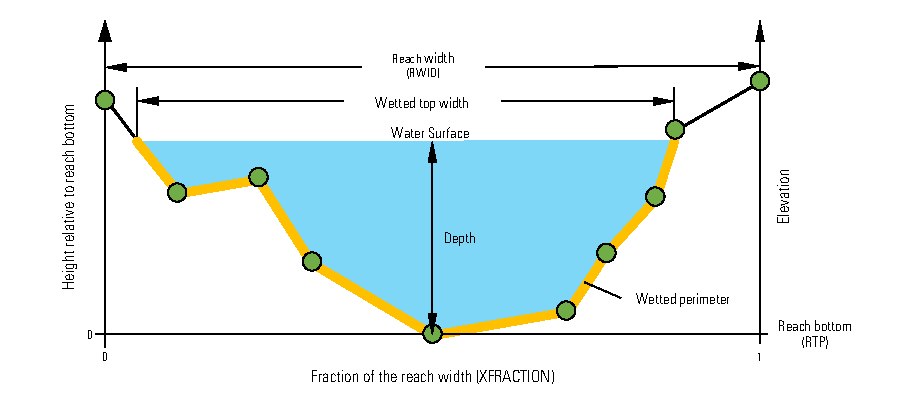
\includegraphics[scale=1.0]{../Figures/n-point-cross-section}
	\caption[Illustration of a irregular cross section used to compute depth, wetted top width, wetted perimeter, and wetted cross-sectional area for a stream reach]{Irregular cross section used to compute depth, wetted top width, wetted perimeter, and wetted cross-sectional area for a stream reach for the case where the maximum XFRACTION is one}
	\label{fig:sfr-n-point}
\end{figure}

Where irregular cross sections are used to define cross-sectional stream geometries, the wetted perimeter used in Manning’s equation [Equation 7-7, \cite{modflow6gwf}] depends on the number of points defining the cross section and the simulated stage.  Using only the minimum number of points (i.e., 2-point cross section), \mf does not include perimeter lengths above the uppermost defined points in the wetted perimeter calculations. For example, the 2-point cross sections shown in fig.~\ref{fig:sfr-n-point-wp}A-C depict the cross-sectional areas (light blue) and wetted perimeters (orange) calculated by the SFR package and used in \cite{modflow6gwf} (Equation 7-7).  In applications where the intent is for the wetted perimeter to include the entire lengths of wetted sides, additional points above the maximum anticipated stage should be defined (fig.~\ref{fig:sfr-n-point-wp}D).  Note that when the simulated stream stage rises above the points representing the top of the channel, the additional cross-sectional flow area above the defined points will be accounted for but the corresponding wetted perimeter will not extend above the defined points (fig.~\ref{fig:sfr-n-point-wp}E,F).


\begin{figure}[ht]
	\centering
	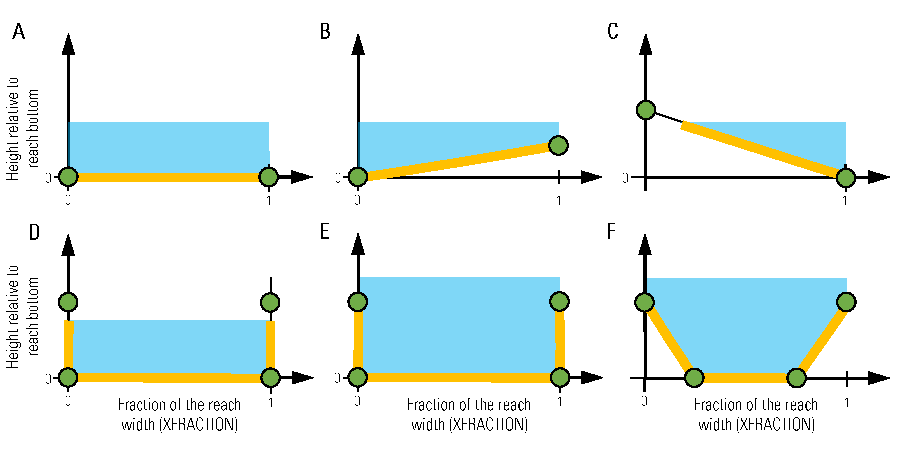
\includegraphics[scale=1.0]{../Figures/n-point-cross-section-wetted-perimeter}
	\caption[Illustrations of variously defined n-point cross-sections that show how wetted perimeter will vary depending on the stage and the number of points used to define the cross-section]{Example irregular cross-section geometries showing the corresponding wetted perimeter based on the number of points that define a cross-section and the simulated stage.  (A-C) Wetted perimeters (orange lines) for variously configured 2-point cross-sections.  (D-F) Wetted perimeters for variously configured 4-point cross-sections}
	\label{fig:sfr-n-point-wp}
\end{figure}

Cross-Section tables are specified by including file names in the CROSSSECTIONS or PERIOD blocks of the SFR Package for specific reaches.  These file names correspond to a Streamflow Routing cross-section table input file.  The format of the Streamflow Routing cross-section table input file is described here.

\vspace{5mm}
\subsubsection{Structure of Blocks}
\vspace{5mm}

\lstinputlisting[style=blockdefinition]{./mf6ivar/tex/utl-sfrtab-dimensions.dat}
\lstinputlisting[style=blockdefinition]{./mf6ivar/tex/utl-sfrtab-table.dat}
\vspace{5mm}

\vspace{5mm}
\subsubsection{Explanation of Variables}
\begin{description}
% DO NOT MODIFY THIS FILE DIRECTLY.  IT IS CREATED BY mf6ivar.py 

\item \textbf{Block: DIMENSIONS}

\begin{description}
\item \texttt{nrow}---integer value specifying the number of rows in the reach cross-section table. There must be NROW rows of data in the TABLE block.

\item \texttt{ncol}---integer value specifying the number of columns in the reach cross-section table. There must be NCOL columns of data in the TABLE block. NCOL must be equal to 2 if MANFRACTION is not specified or 3 otherwise.

\end{description}
\item \textbf{Block: TABLE}

\begin{description}
\item \texttt{xfraction}---real value that defines the station (x) data for the cross-section as a fraction of the width (RWID) of the reach. XFRACTION must be greater than or equal to zero but can be greater than one. XFRACTION values can be used to decrease or increase the width of a reach from the specified reach width (RWID).

\item \texttt{height}---real value that is the height relative to the top of the lowest elevation of the streambed (RTP) and corresponding to the station data on the same line. HEIGHT must be greater than or equal to zero and at least one cross-section height must be equal to zero.

\item \texttt{manfraction}---real value that defines the Manning's roughness coefficient data for the cross-section as a fraction of the Manning's roughness coefficient for the reach (MAN) and corresponding to the station data on the same line. MANFRACTION must be greater than zero. MANFRACTION is applied from the XFRACTION value on the same line to the XFRACTION value on the next line. Although a MANFRACTION value is specified on the last line, any value greater than zero can be applied to MANFRACTION(NROW). MANFRACTION is only specified if NCOL is 3. If MANFRACTION is not specified, the Manning's roughness coefficient for the reach (MAN) is applied to the entire cross-section.

\end{description}


\end{description}

\subsubsection{Example Input File}
\lstinputlisting[style=inputfile]{./mf6ivar/examples/utl-sfrtab-example.dat}



\newpage
\subsection{Lake (LAK) Package}
Input to the Lake (LAK) Package is read from the file that has type ``LAK6'' in the Name File.  Any number of LAK Packages can be specified for a single groundwater flow model.

\vspace{5mm}
\subsubsection{Structure of Blocks}
\vspace{5mm}

\noindent \textit{FOR EACH SIMULATION}
\lstinputlisting[style=blockdefinition]{./mf6ivar/tex/gwf-lak-options.dat}
\lstinputlisting[style=blockdefinition]{./mf6ivar/tex/gwf-lak-dimensions.dat}
\lstinputlisting[style=blockdefinition]{./mf6ivar/tex/gwf-lak-packagedata.dat}
\noindent \textit{IF \texttt{nlakeconn} IS GREATER THAN ZERO FOR ANY LAKE}
\lstinputlisting[style=blockdefinition]{./mf6ivar/tex/gwf-lak-connectiondata.dat}
\noindent \textit{IF \texttt{ntables} IS GREATER THAN ZERO}
\lstinputlisting[style=blockdefinition]{./mf6ivar/tex/gwf-lak-tables.dat}
\noindent \textit{IF \texttt{noutlets} IS GREATER THAN ZERO FOR ANY LAKE}
\lstinputlisting[style=blockdefinition]{./mf6ivar/tex/gwf-lak-outlets.dat}

\vspace{5mm}
\noindent \textit{FOR ANY STRESS PERIOD}
\lstinputlisting[style=blockdefinition]{./mf6ivar/tex/gwf-lak-period.dat}
\advancedpackageperioddescription{lake}{lakes}

\vspace{5mm}
\subsubsection{Explanation of Variables}
\begin{description}
% DO NOT MODIFY THIS FILE DIRECTLY.  IT IS CREATED BY mf6ivar.py 

\item \textbf{Block: OPTIONS}

\begin{description}
\item \texttt{auxiliary}---defines an array of one or more auxiliary variable names.  There is no limit on the number of auxiliary variables that can be provided on this line; however, lists of information provided in subsequent blocks must have a column of data for each auxiliary variable name defined here.   The number of auxiliary variables detected on this line determines the value for naux.  Comments cannot be provided anywhere on this line as they will be interpreted as auxiliary variable names.  Auxiliary variables may not be used by the package, but they will be available for use by other parts of the program.  The program will terminate with an error if auxiliary variables are specified on more than one line in the options block.

\item \texttt{BOUNDNAMES}---keyword to indicate that boundary names may be provided with the list of lake cells.

\item \texttt{PRINT\_INPUT}---keyword to indicate that the list of lake information will be written to the listing file immediately after it is read.

\item \texttt{PRINT\_STAGE}---keyword to indicate that the list of lake stages will be printed to the listing file for every stress period in which ``HEAD PRINT'' is specified in Output Control.  If there is no Output Control option and PRINT\_STAGE is specified, then stages are printed for the last time step of each stress period.

\item \texttt{PRINT\_FLOWS}---keyword to indicate that the list of lake flow rates will be printed to the listing file for every stress period time step in which ``BUDGET PRINT'' is specified in Output Control.  If there is no Output Control option and ``PRINT\_FLOWS'' is specified, then flow rates are printed for the last time step of each stress period.

\item \texttt{SAVE\_FLOWS}---keyword to indicate that lake flow terms will be written to the file specified with ``BUDGET FILEOUT'' in Output Control.

\item \texttt{STAGE}---keyword to specify that record corresponds to stage.

\item \texttt{stagefile}---name of the binary output file to write stage information.

\item \texttt{BUDGET}---keyword to specify that record corresponds to the budget.

\item \texttt{FILEOUT}---keyword to specify that an output filename is expected next.

\item \texttt{budgetfile}---name of the binary output file to write budget information.

\item \texttt{BUDGETCSV}---keyword to specify that record corresponds to the budget CSV.

\item \texttt{budgetcsvfile}---name of the comma-separated value (CSV) output file to write budget summary information.  A budget summary record will be written to this file for each time step of the simulation.

\item \texttt{PACKAGE\_CONVERGENCE}---keyword to specify that record corresponds to the package convergence comma spaced values file.

\item \texttt{package\_convergence\_filename}---name of the comma spaced values output file to write package convergence information.

\item \texttt{TS6}---keyword to specify that record corresponds to a time-series file.

\item \texttt{FILEIN}---keyword to specify that an input filename is expected next.

\item \texttt{ts6\_filename}---defines a time-series file defining time series that can be used to assign time-varying values. See the ``Time-Variable Input'' section for instructions on using the time-series capability.

\item \texttt{OBS6}---keyword to specify that record corresponds to an observations file.

\item \texttt{obs6\_filename}---name of input file to define observations for the LAK package. See the ``Observation utility'' section for instructions for preparing observation input files. Tables \ref{table:gwf-obstypetable} and \ref{table:gwt-obstypetable} lists observation type(s) supported by the LAK package.

\item \texttt{MOVER}---keyword to indicate that this instance of the LAK Package can be used with the Water Mover (MVR) Package.  When the MOVER option is specified, additional memory is allocated within the package to store the available, provided, and received water.

\item \texttt{surfdep}---real value that defines the surface depression depth for VERTICAL lake-GWF connections. If specified, SURFDEP must be greater than or equal to zero. If SURFDEP is not specified, a default value of zero is used for all vertical lake-GWF connections.

\item \texttt{time\_conversion}---real value that is used to convert user-specified Manning's roughness coefficients or gravitational acceleration used to calculate outlet flows from seconds to model time units. TIME\_CONVERSION should be set to 1.0, 60.0, 3,600.0, 86,400.0, and 31,557,600.0 when using time units (TIME\_UNITS) of seconds, minutes, hours, days, or years in the simulation, respectively. CONVTIME does not need to be specified if no lake outlets are specified or TIME\_UNITS are seconds.

\item \texttt{length\_conversion}---real value that is used to convert outlet user-specified Manning's roughness coefficients or gravitational acceleration used to calculate outlet flows from meters to model length units. LENGTH\_CONVERSION should be set to 3.28081, 1.0, and 100.0 when using length units (LENGTH\_UNITS) of feet, meters, or centimeters in the simulation, respectively. LENGTH\_CONVERSION does not need to be specified if no lake outlets are specified or LENGTH\_UNITS are meters.

\end{description}
\item \textbf{Block: DIMENSIONS}

\begin{description}
\item \texttt{nlakes}---value specifying the number of lakes that will be simulated for all stress periods.

\item \texttt{noutlets}---value specifying the number of outlets that will be simulated for all stress periods. If NOUTLETS is not specified, a default value of zero is used.

\item \texttt{ntables}---value specifying the number of lakes tables that will be used to define the lake stage, volume relation, and surface area. If NTABLES is not specified, a default value of zero is used.

\end{description}
\item \textbf{Block: PACKAGEDATA}

\begin{description}
\item \texttt{lakeno}---integer value that defines the lake number associated with the specified PACKAGEDATA data on the line. LAKENO must be greater than zero and less than or equal to NLAKES. Lake information must be specified for every lake or the program will terminate with an error.  The program will also terminate with an error if information for a lake is specified more than once.

\item \texttt{strt}---real value that defines the starting stage for the lake.

\item \texttt{nlakeconn}---integer value that defines the number of GWF cells connected to this (LAKENO) lake. There can only be one vertical lake connection to each GWF cell. NLAKECONN must be greater than zero.

\item \textcolor{blue}{\texttt{aux}---represents the values of the auxiliary variables for each lake. The values of auxiliary variables must be present for each lake. The values must be specified in the order of the auxiliary variables specified in the OPTIONS block.  If the package supports time series and the Options block includes a TIMESERIESFILE entry (see the ``Time-Variable Input'' section), values can be obtained from a time series by entering the time-series name in place of a numeric value.}

\item \texttt{boundname}---name of the lake cell.  BOUNDNAME is an ASCII character variable that can contain as many as 40 characters.  If BOUNDNAME contains spaces in it, then the entire name must be enclosed within single quotes.

\end{description}
\item \textbf{Block: CONNECTIONDATA}

\begin{description}
\item \texttt{lakeno}---integer value that defines the lake number associated with the specified CONNECTIONDATA data on the line. LAKENO must be greater than zero and less than or equal to NLAKES. Lake connection information must be specified for every lake connection to the GWF model (NLAKECONN) or the program will terminate with an error.  The program will also terminate with an error if connection information for a lake connection to the GWF model is specified more than once.

\item \texttt{iconn}---integer value that defines the GWF connection number for this lake connection entry. ICONN must be greater than zero and less than or equal to NLAKECONN for lake LAKENO.

\item \texttt{cellid}---is the cell identifier, and depends on the type of grid that is used for the simulation.  For a structured grid that uses the DIS input file, CELLID is the layer, row, and column.   For a grid that uses the DISV input file, CELLID is the layer and CELL2D number.  If the model uses the unstructured discretization (DISU) input file, CELLID is the node number for the cell.

\item \texttt{claktype}---character string that defines the lake-GWF connection type for the lake connection. Possible lake-GWF connection type strings include:  VERTICAL--character keyword to indicate the lake-GWF connection is vertical  and connection conductance calculations use the hydraulic conductivity corresponding to the $K_{33}$ tensor component defined for CELLID in the NPF package. HORIZONTAL--character keyword to indicate the lake-GWF connection is horizontal and connection conductance calculations use the hydraulic conductivity corresponding to the $K_{11}$ tensor component defined for CELLID in the NPF package. EMBEDDEDH--character keyword to indicate the lake-GWF connection is embedded in a single cell and connection conductance calculations use the hydraulic conductivity corresponding to the $K_{11}$ tensor component defined for CELLID in the NPF package. EMBEDDEDV--character keyword to indicate the lake-GWF connection is embedded in a single cell and connection conductance calculations use the hydraulic conductivity corresponding to the $K_{33}$ tensor component defined for CELLID in the NPF package. Embedded lakes can only be connected to a single cell (NLAKECONN = 1) and there must be a lake table associated with each embedded lake.

\item \texttt{bedleak}---character string or real value that defines the bed leakance for the lake-GWF connection. BEDLEAK must be greater than or equal to zero or specified to be NONE. If BEDLEAK is specified to be NONE, the lake-GWF connection conductance is solely a function of aquifer properties in the connected GWF cell and lakebed sediments are assumed to be absent.

\item \texttt{belev}---real value that defines the bottom elevation for a HORIZONTAL lake-GWF connection. Any value can be specified if CLAKTYPE is VERTICAL, EMBEDDEDH, or EMBEDDEDV. If CLAKTYPE is HORIZONTAL and BELEV is not equal to TELEV, BELEV must be greater than or equal to the bottom of the GWF cell CELLID. If BELEV is equal to TELEV, BELEV is reset to the bottom of the GWF cell CELLID.

\item \texttt{telev}---real value that defines the top elevation for a HORIZONTAL lake-GWF connection. Any value can be specified if CLAKTYPE is VERTICAL, EMBEDDEDH, or EMBEDDEDV. If CLAKTYPE is HORIZONTAL and TELEV is not equal to BELEV, TELEV must be less than or equal to the top of the GWF cell CELLID. If TELEV is equal to BELEV, TELEV is reset to the top of the GWF cell CELLID.

\item \texttt{connlen}---real value that defines the distance between the connected GWF CELLID node and the lake for a HORIZONTAL, EMBEDDEDH, or EMBEDDEDV lake-GWF connection. CONLENN must be greater than zero for a HORIZONTAL, EMBEDDEDH, or EMBEDDEDV lake-GWF connection. Any value can be specified if CLAKTYPE is VERTICAL.

\item \texttt{connwidth}---real value that defines the connection face width for a HORIZONTAL lake-GWF connection. CONNWIDTH must be greater than zero for a HORIZONTAL lake-GWF connection. Any value can be specified if CLAKTYPE is VERTICAL, EMBEDDEDH, or EMBEDDEDV.

\end{description}
\item \textbf{Block: TABLES}

\begin{description}
\item \texttt{lakeno}---integer value that defines the lake number associated with the specified TABLES data on the line. LAKENO must be greater than zero and less than or equal to NLAKES. The program will terminate with an error if table information for a lake is specified more than once or the number of specified tables is less than NTABLES.

\item \texttt{TAB6}---keyword to specify that record corresponds to a table file.

\item \texttt{FILEIN}---keyword to specify that an input filename is expected next.

\item \texttt{tab6\_filename}---character string that defines the path and filename for the file containing lake table data for the lake connection. The TAB6\_FILENAME file includes the number of entries in the file and the relation between stage, volume, and surface area for each entry in the file. Lake table files for EMBEDDEDH and EMBEDDEDV lake-GWF connections also include lake-GWF exchange area data for each entry in the file. Instructions for creating the TAB6\_FILENAME input file are provided in Lake Table Input File section.

\end{description}
\item \textbf{Block: OUTLETS}

\begin{description}
\item \texttt{outletno}---integer value that defines the outlet number associated with the specified OUTLETS data on the line. OUTLETNO must be greater than zero and less than or equal to NOUTLETS. Outlet information must be specified for every outlet or the program will terminate with an error. The program will also terminate with an error if information for a outlet is specified more than once.

\item \texttt{lakein}---integer value that defines the lake number that outlet is connected to. LAKEIN must be greater than zero and less than or equal to NLAKES.

\item \texttt{lakeout}---integer value that defines the lake number that outlet discharge from lake outlet OUTLETNO is routed to. LAKEOUT must be greater than or equal to zero and less than or equal to NLAKES. If LAKEOUT is zero, outlet discharge from lake outlet OUTLETNO is discharged to an external boundary.

\item \texttt{couttype}---character string that defines the outlet type for the outlet OUTLETNO. Possible COUTTYPE strings include: SPECIFIED--character keyword to indicate the outlet is defined as a specified flow.  MANNING--character keyword to indicate the outlet is defined using Manning's equation. WEIR--character keyword to indicate the outlet is defined using a sharp weir equation.

\item \textcolor{blue}{\texttt{invert}---real value that defines the invert elevation for the lake outlet. Any value can be specified if COUTTYPE is SPECIFIED. If the Options block includes a TIMESERIESFILE entry (see the ``Time-Variable Input'' section), values can be obtained from a time series by entering the time-series name in place of a numeric value.}

\item \textcolor{blue}{\texttt{width}---real value that defines the width of the lake outlet. Any value can be specified if COUTTYPE is SPECIFIED. If the Options block includes a TIMESERIESFILE entry (see the ``Time-Variable Input'' section), values can be obtained from a time series by entering the time-series name in place of a numeric value.}

\item \textcolor{blue}{\texttt{rough}---real value that defines the roughness coefficient for the lake outlet. Any value can be specified if COUTTYPE is not MANNING. If the Options block includes a TIMESERIESFILE entry (see the ``Time-Variable Input'' section), values can be obtained from a time series by entering the time-series name in place of a numeric value.}

\item \textcolor{blue}{\texttt{slope}---real value that defines the bed slope for the lake outlet. Any value can be specified if COUTTYPE is not MANNING. If the Options block includes a TIMESERIESFILE entry (see the ``Time-Variable Input'' section), values can be obtained from a time series by entering the time-series name in place of a numeric value.}

\end{description}
\item \textbf{Block: PERIOD}

\begin{description}
\item \texttt{iper}---integer value specifying the starting stress period number for which the data specified in the PERIOD block apply.  IPER must be less than or equal to NPER in the TDIS Package and greater than zero.  The IPER value assigned to a stress period block must be greater than the IPER value assigned for the previous PERIOD block.  The information specified in the PERIOD block will continue to apply for all subsequent stress periods, unless the program encounters another PERIOD block.

\item \texttt{number}---integer value that defines the lake or outlet number associated with the specified PERIOD data on the line.  NUMBER must be greater than zero and less than or equal to NLAKES for a lake number and less than or equal to NOUTLETS for an outlet number.

\item \texttt{laksetting}---line of information that is parsed into a keyword and values.  Keyword values that can be used to start the LAKSETTING string include both keywords for lake settings and keywords for outlet settings.  Keywords for lake settings include: STATUS, STAGE, RAINFALL, EVAPORATION, RUNOFF, INFLOW, WITHDRAWAL, and AUXILIARY.  Keywords for outlet settings include RATE, INVERT, WIDTH, SLOPE, and ROUGH.

\begin{lstlisting}[style=blockdefinition]
STATUS <status>
STAGE <@stage@>
RAINFALL <@rainfall@>
EVAPORATION <@evaporation@>
RUNOFF <@runoff@>
INFLOW <@inflow@>
WITHDRAWAL <@withdrawal@>
RATE <@rate@>
INVERT <@invert@>
WIDTH <@width@>
SLOPE <@slope@>
ROUGH <@rough@>
AUXILIARY <auxname> <@auxval@> 
\end{lstlisting}

\item \texttt{status}---keyword option to define lake status.  STATUS can be ACTIVE, INACTIVE, or CONSTANT. By default, STATUS is ACTIVE.

\item \textcolor{blue}{\texttt{stage}---real or character value that defines the stage for the lake. The specified STAGE is only applied if the lake is a constant stage lake. If the Options block includes a TIMESERIESFILE entry (see the ``Time-Variable Input'' section), values can be obtained from a time series by entering the time-series name in place of a numeric value.}

\item \textcolor{blue}{\texttt{rainfall}---real or character value that defines the rainfall rate $(LT^{-1})$ for the lake. Value must be greater than or equal to zero. If the Options block includes a TIMESERIESFILE entry (see the ``Time-Variable Input'' section), values can be obtained from a time series by entering the time-series name in place of a numeric value.}

\item \textcolor{blue}{\texttt{evaporation}---real or character value that defines the maximum evaporation rate $(LT^{-1})$ for the lake. Value must be greater than or equal to zero. If the Options block includes a TIMESERIESFILE entry (see the ``Time-Variable Input'' section), values can be obtained from a time series by entering the time-series name in place of a numeric value.}

\item \textcolor{blue}{\texttt{runoff}---real or character value that defines the runoff rate $(L^3 T^{-1})$ for the lake. Value must be greater than or equal to zero. If the Options block includes a TIMESERIESFILE entry (see the ``Time-Variable Input'' section), values can be obtained from a time series by entering the time-series name in place of a numeric value.}

\item \textcolor{blue}{\texttt{inflow}---real or character value that defines the volumetric inflow rate $(L^3 T^{-1})$ for the lake. Value must be greater than or equal to zero. If the Options block includes a TIMESERIESFILE entry (see the ``Time-Variable Input'' section), values can be obtained from a time series by entering the time-series name in place of a numeric value. By default, inflow rates are zero for each lake.}

\item \textcolor{blue}{\texttt{withdrawal}---real or character value that defines the maximum withdrawal rate $(L^3 T^{-1})$ for the lake. Value must be greater than or equal to zero. If the Options block includes a TIMESERIESFILE entry (see the ``Time-Variable Input'' section), values can be obtained from a time series by entering the time-series name in place of a numeric value.}

\item \textcolor{blue}{\texttt{rate}---real or character value that defines the extraction rate for the lake outflow. A positive value indicates inflow and a negative value indicates outflow from the lake. RATE only applies to active (IBOUND $>$ 0) lakes. A specified RATE is only applied if COUTTYPE for the OUTLETNO is SPECIFIED. If the Options block includes a TIMESERIESFILE entry (see the ``Time-Variable Input'' section), values can be obtained from a time series by entering the time-series name in place of a numeric value. By default, the RATE for each SPECIFIED lake outlet is zero.}

\item \textcolor{blue}{\texttt{invert}---real or character value that defines the invert elevation for the lake outlet. A specified INVERT value is only used for active lakes if COUTTYPE for lake outlet OUTLETNO is not SPECIFIED. If the Options block includes a TIMESERIESFILE entry (see the ``Time-Variable Input'' section), values can be obtained from a time series by entering the time-series name in place of a numeric value.}

\item \textcolor{blue}{\texttt{rough}---real value that defines the roughness coefficient for the lake outlet. Any value can be specified if COUTTYPE is not MANNING. If the Options block includes a TIMESERIESFILE entry (see the ``Time-Variable Input'' section), values can be obtained from a time series by entering the time-series name in place of a numeric value.}

\item \textcolor{blue}{\texttt{width}---real or character value that defines the width of the lake outlet. A specified WIDTH value is only used for active lakes if COUTTYPE for lake outlet OUTLETNO is not SPECIFIED. If the Options block includes a TIMESERIESFILE entry (see the ``Time-Variable Input'' section), values can be obtained from a time series by entering the time-series name in place of a numeric value.}

\item \textcolor{blue}{\texttt{slope}---real or character value that defines the bed slope for the lake outlet. A specified SLOPE value is only used for active lakes if COUTTYPE for lake outlet OUTLETNO is MANNING. If the Options block includes a TIMESERIESFILE entry (see the ``Time-Variable Input'' section), values can be obtained from a time series by entering the time-series name in place of a numeric value.}

\item \texttt{AUXILIARY}---keyword for specifying auxiliary variable.

\item \texttt{auxname}---name for the auxiliary variable to be assigned AUXVAL.  AUXNAME must match one of the auxiliary variable names defined in the OPTIONS block. If AUXNAME does not match one of the auxiliary variable names defined in the OPTIONS block the data are ignored.

\item \textcolor{blue}{\texttt{auxval}---value for the auxiliary variable. If the Options block includes a TIMESERIESFILE entry (see the ``Time-Variable Input'' section), values can be obtained from a time series by entering the time-series name in place of a numeric value.}

\end{description}


\end{description}

\vspace{5mm}
\subsubsection{Example Input File}
\lstinputlisting[style=inputfile]{./mf6ivar/examples/gwf-lak-example.dat}

\vspace{5mm}
\subsubsection{Available observation types}
Lake Package observations include lake stage and all of the terms that contribute to the continuity equation for each lake. Additional LAK Package observations include flow rates for individual outlets, lakes, or groups of lakes (\texttt{outlet}); the lake volume (\texttt{volume}); lake surface area (\texttt{surface-area}); wetted area for a lake-aquifer connection (\texttt{wetted-area}); and the conductance for a lake-aquifer connection conductance (\texttt{conductance}). The data required for each LAK Package observation type is defined in table~\ref{table:gwf-lakobstype}. Negative and positive values for \texttt{lak} observations represent a loss from and gain to the GWF model, respectively. For all other flow terms, negative and positive values represent a loss from and gain from the LAK package, respectively.

\begin{longtable}{p{2cm} p{2.75cm} p{2cm} p{1.25cm} p{7cm}}
\caption{Available LAK Package observation types} \tabularnewline

\hline
\hline
\textbf{Stress Package} & \textbf{Observation type} & \textbf{ID} & \textbf{ID2} & \textbf{Description} \\
\hline
\endfirsthead

\captionsetup{textformat=simple}
\caption*{\textbf{Table \arabic{table}.}{\quad}Available LAK Package observation types.---Continued} \tabularnewline

\hline
\hline
\textbf{Stress Package} & \textbf{Observation type} & \textbf{ID} & \textbf{ID2} & \textbf{Description} \\
\hline
\endhead


\hline
\endfoot

LAK & stage & ifno or boundname & -- & Surface-water stage in a lake. If boundname is specified, boundname must be unique for each lake. \\
LAK & ext-inflow & ifno or boundname & -- & Specified inflow into a lake or group of lakes. \\
LAK & outlet-inflow & ifno or boundname & -- & Simulated inflow from upstream lake outlets into a lake or group of lakes. \\
LAK & inflow & ifno or boundname & -- & Sum of specified inflow and simulated inflow from upstream lake outlets into a lake or group of lakes. \\
LAK & from-mvr & ifno or boundname & -- & Inflow into a lake or group of lakes from the MVR package. \\
LAK & rainfall & ifno or boundname & -- & Rainfall rate applied to a lake or group of lakes. \\
LAK & runoff & ifno or boundname & -- & Runoff rate applied to a lake or group of lakes. \\
LAK & lak & ifno or boundname & \texttt{iconn} or -- & Simulated flow rate for a lake or group of lakes and its aquifer connection(s). If boundname is not specified for ID, then the simulated lake-aquifer flow rate at a specific lake connection is observed. In this case, ID2 must be specified and is the connection number \texttt{iconn}. \\
LAK & withdrawal & ifno or boundname & -- & Specified withdrawal rate from a lake or group of lakes. \\
LAK & evaporation & ifno or boundname & -- & Simulated evaporation rate from a lake or group of lakes. \\
LAK & ext-outflow & outletno or boundname & -- & External outflow from a lake outlet, a lake, or a group of lakes to an external boundary. If boundname is not specified for ID, then the external outflow from a specific lake outlet is observed. In this case, ID is the outlet number outletno. \\
LAK & to-mvr & outletno or boundname & -- & Outflow from a lake outlet, a lake, or a group of lakes that is available for the MVR package. If boundname is not specified for ID, then the outflow available for the MVR package from a specific lake outlet is observed. In this case, ID is the outlet number outletno. \\
LAK & storage & ifno or boundname & -- & Simulated storage flow rate for a lake or group of lakes. \\
LAK & constant & ifno or boundname & -- & Simulated constant-flow rate for a lake or group of lakes. \\
LAK & outlet & outletno or boundname & -- & Simulated outlet flow rate from a lake outlet, a lake, or a group of lakes. If boundname is not specified for ID, then the flow from a specific lake outlet is observed. In this case, ID is the outlet number outletno. \\
LAK & volume & ifno or boundname & -- & Simulated lake volume or group of lakes. \\
LAK & surface-area & ifno or boundname & -- & Simulated surface area for a lake or group of lakes. \\
LAK & wetted-area & ifno or boundname & \texttt{iconn} or -- & Simulated wetted-area for a lake or group of lakes and its aquifer connection(s). If boundname is not specified for ID, then the wetted area of a specific lake connection is observed. In this case, ID2 must be specified and is the connection number \texttt{iconn}. \\
LAK & conductance & ifno or boundname & \texttt{iconn} or -- & Calculated conductance for a lake or group of lakes and its aquifer connection(s). If boundname is not specified for ID, then the calculated conductance of a specific lake connection is observed. In this case, ID2 must be specified and is the connection number \texttt{iconn}.

\label{table:gwf-lakobstype}
\end{longtable}

\vspace{5mm}
\subsubsection{Example Observation Input File}
\lstinputlisting[style=inputfile]{./mf6ivar/examples/gwf-lak-example-obs.dat}

\newpage
\subsection{Lake Table Input File}
Lake tables of stage, volume, and surface area can be specified for individual lakes.  Lake tables are specified by including file names in the LAKE\_TABLES block of the LAK Package.  These file names correspond to a lake table input file.  The format of the lake table input file is described here.

\vspace{5mm}
\subsubsection{Structure of Blocks}
\vspace{5mm}

\lstinputlisting[style=blockdefinition]{./mf6ivar/tex/utl-laktab-dimensions.dat}
\lstinputlisting[style=blockdefinition]{./mf6ivar/tex/utl-laktab-table.dat}
\vspace{5mm}

\vspace{5mm}
\subsubsection{Explanation of Variables}
\begin{description}
% DO NOT MODIFY THIS FILE DIRECTLY.  IT IS CREATED BY mf6ivar.py 

\item \textbf{Block: DIMENSIONS}

\begin{description}
\item \texttt{nrow}---integer value specifying the number of rows in the lake table. There must be NROW rows of data in the TABLE block.

\item \texttt{ncol}---integer value specifying the number of columns in the lake table. There must be NCOL columns of data in the TABLE block. For lakes with HORIZONTAL and/or VERTICAL CTYPE connections, NCOL must be equal to 3. For lakes with EMBEDDEDH or EMBEDDEDV CTYPE connections, NCOL must be equal to 4.

\end{description}
\item \textbf{Block: TABLE}

\begin{description}
\item \texttt{stage}---real value that defines the stage corresponding to the remaining data on the line.

\item \texttt{volume}---real value that defines the lake volume corresponding to the stage specified on the line.

\item \texttt{sarea}---real value that defines the lake surface area corresponding to the stage specified on the line.

\item \texttt{barea}---real value that defines the lake-GWF exchange area corresponding to the stage specified on the line. BAREA is only specified if the CLAKTYPE for the lake is EMBEDDEDH or EMBEDDEDV.

\end{description}


\end{description}

\subsubsection{Example Input File}
\lstinputlisting[style=inputfile]{./mf6ivar/examples/utl-laktab-example.dat}



\newpage
\subsection{Unsaturated Zone Flow (UZF) Package}
\input{gwf/uzf}

\newpage
\subsection{Water Mover (MVR) Package}
The MVR Package can be used to transfer water from a provider to a receiver.  Providers are extraction wells, streamflow routing reaches, lakes and other model features that can be conceptualized as having water available.  The list of packages that can provide water to the MVR Package are:

\begin{itemize}
  \item Well Package
  \item Drain Package
  \item River Package
  \item General-Head Boundary Package
  \item Multi-Aquifer Well Package
  \item Streamflow Routing Package
  \item Unsaturated Zone Flow Package
  \item Lake Package
\end{itemize}

Receivers are package features within the model that solve a continuity equation of inflows, outflows, and change in storage.  These features include multi-aquifer wells, streamflow routing reaches, lakes, and unsaturated zone flow cells.  The list of packages that can receive water is shorter than the provider list, because the WEL, DRN, RIV, and GHB Packages do not represent a continuity equation (boundary stages or elevations are specified by the user).  Therefore, the list of packages that can act as receivers are:

\begin{itemize}
  \item Multi-Aquifer Well Package
  \item Streamflow Routing Package
  \item Unsaturated Zone Flow Package
  \item Lake Package
\end{itemize}

\noindent The program will terminate with an error if the MVR is used with an unsupported package type.

The MVR Package is based on the calculation of available water that can be moved from one package feature to another.  The equations used to determine how much water can be transferred are as follows, where $Q_P$ is the flow rate that can be supported by the provider (the available flow rate), and $Q_R$ is the actual rate of water transferred to the receiver.

\begin{enumerate}
\item A FACTOR can be specified such that 

$Q_R = \alpha Q_P$

\noindent where $\alpha$ is the factor to convert the provider flow rate to the receiver flow rate.

\item An EXCESS rate can be specified by the user as $Q_S$ such that

\[
    Q_R = 
\begin{cases}
    Q_P - Q_S, & \text{if } Q_P > Q_S \\
    0,              & \text{otherwise}
\end{cases}
\]

\noindent In the EXCESS case, any water that exceeds the user specified rate is provided to the receiver.  No water is provided to the receiver if the available water is less than the user specified value.

\item A THRESHOLD rate can be specified for $Q_S$ such that

\[
    Q_R = 
\begin{cases}
    0, & \text{if } Q_S > Q_P \\
    Q_S,              & \text{otherwise}
\end{cases}
\]

\noindent In the THRESHOLD case, no flow is provided to the receiver until the available water exceeds the user specified $Q_S$ rate.  Once the available water exceeds the user specified rate, then the $Q_S$ rate is provided to the receiver.

\item An UPTO rate can be specified for $Q_S$ such that

\[
    Q_R = 
\begin{cases}
    Q_S, & \text{if } Q_P > Q_S \\
    Q_P,              & \text{otherwise}
\end{cases}
\]

\noindent In the UPTO case, all of the available water will be taken from the provider up to the $Q_S$ value specified by the user.  Once $Q_S$ is exceeded, the receiver will continue to get the $Q_S$ value specified by the user.
\end{enumerate}

\noindent In the MVR PERIOD block (as shown below), the user assigns the equation used for each individual entry by specifying FACTOR, EXCESS, THRESHOLD, or UPTO to the input variable \texttt{mvrtype}.

Input to the Water Mover (MVR) Package is read from the file that has type ``MVR6'' in the Name File.  Only one MVR Package can be used per GWF Model.

\vspace{5mm}
\subsubsection{Structure of Blocks}
\vspace{5mm}

\noindent \textit{FOR EACH SIMULATION}
\lstinputlisting[style=blockdefinition]{./mf6ivar/tex/gwf-mvr-options.dat}
\lstinputlisting[style=blockdefinition]{./mf6ivar/tex/gwf-mvr-dimensions.dat}
\lstinputlisting[style=blockdefinition]{./mf6ivar/tex/gwf-mvr-packages.dat}
\vspace{5mm}
\noindent \textit{FOR ANY STRESS PERIOD}
\lstinputlisting[style=blockdefinition]{./mf6ivar/tex/gwf-mvr-period.dat}
All of the mover information in the PERIOD block will continue to apply for subsequent stress periods until the end of the simulation, or until another PERIOD block is encountered.  When a new PERIOD block is encountered, all of the movers from the previous block are replaced with the movers in the new PERIOD block.  Note that this behavior is different from the other advanced packages (MAW, SFR, LAK, and UZF).  To turn off all of the movers for a stress period, a PERIOD block must be specified with no entries.  If a PERIOD block is not specified for the first stress period, then no movers will be applied until the \texttt{iper} value of the first PERIOD block in the file.


\vspace{5mm}
\subsubsection{Explanation of Variables}
\begin{description}
% DO NOT MODIFY THIS FILE DIRECTLY.  IT IS CREATED BY mf6ivar.py 

\item \textbf{Block: OPTIONS}

\begin{description}
\item \texttt{PRINT\_INPUT}---keyword to indicate that the list of MVR information will be written to the listing file immediately after it is read.

\item \texttt{PRINT\_FLOWS}---keyword to indicate that the list of MVR flow rates will be printed to the listing file for every stress period time step in which ``BUDGET PRINT'' is specified in Output Control.  If there is no Output Control option and ``PRINT\_FLOWS'' is specified, then flow rates are printed for the last time step of each stress period.

\item \texttt{MODELNAMES}---keyword to indicate that all package names will be preceded by the model name for the package.  Model names are required when the Mover Package is used with a GWF-GWF Exchange.  The MODELNAME keyword should not be used for a Mover Package that is for a single GWF Model.

\item \texttt{BUDGET}---keyword to specify that record corresponds to the budget.

\item \texttt{FILEOUT}---keyword to specify that an output filename is expected next.

\item \texttt{budgetfile}---name of the output file to write budget information.

\item \texttt{BUDGETCSV}---keyword to specify that record corresponds to the budget CSV.

\item \texttt{budgetcsvfile}---name of the comma-separated value (CSV) output file to write budget summary information.  A budget summary record will be written to this file for each time step of the simulation.

\end{description}
\item \textbf{Block: DIMENSIONS}

\begin{description}
\item \texttt{maxmvr}---integer value specifying the maximum number of water mover entries that will specified for any stress period.

\item \texttt{maxpackages}---integer value specifying the number of unique packages that are included in this water mover input file.

\end{description}
\item \textbf{Block: PACKAGES}

\begin{description}
\item \texttt{mname}---name of model containing the package.  Model names are assigned by the user in the simulation name file.

\item \texttt{pname}---is the name of a package that may be included in a subsequent stress period block.  The package name is assigned in the name file for the GWF Model.  Package names are optionally provided in the name file.  If they are not provided by the user, then packages are assigned a default value, which is the package acronym followed by a hyphen and the package number.  For example, the first Drain Package is named DRN-1.  The second Drain Package is named DRN-2, and so forth.

\end{description}
\item \textbf{Block: PERIOD}

\begin{description}
\item \texttt{iper}---integer value specifying the starting stress period number for which the data specified in the PERIOD block apply.  IPER must be less than or equal to NPER in the TDIS Package and greater than zero.  The IPER value assigned to a stress period block must be greater than the IPER value assigned for the previous PERIOD block.  The information specified in the PERIOD block will continue to apply for all subsequent stress periods, unless the program encounters another PERIOD block.

\item \texttt{mname1}---name of model containing the package, PNAME1.

\item \texttt{pname1}---is the package name for the provider.  The package PNAME1 must be designated to provide water through the MVR Package by specifying the keyword ``MOVER'' in its OPTIONS block.

\item \texttt{id1}---is the identifier for the provider.  For the standard boundary packages, the provider identifier is the number of the boundary as it is listed in the package input file. (Note that the order of these boundaries may change by stress period, which must be accounted for in the Mover Package.)  So the first well has an identifier of one.  The second is two, and so forth.  For the advanced packages, the identifier is the reach number (SFR Package), well number (MAW Package), or UZF cell number.  For the Lake Package, ID1 is the lake outlet number.  Thus, outflows from a single lake can be routed to different streams, for example.

\item \texttt{mname2}---name of model containing the package, PNAME2.

\item \texttt{pname2}---is the package name for the receiver.  The package PNAME2 must be designated to receive water from the MVR Package by specifying the keyword ``MOVER'' in its OPTIONS block.

\item \texttt{id2}---is the identifier for the receiver.  The receiver identifier is the reach number (SFR Package), Lake number (LAK Package), well number (MAW Package), or UZF cell number.

\item \texttt{mvrtype}---is the character string signifying the method for determining how much water will be moved.  Supported values are ``FACTOR'' ``EXCESS'' ``THRESHOLD'' and ``UPTO''.  These four options determine how the receiver flow rate, $Q_R$, is calculated.  These options mirror the options defined for the cprior variable in the SFR package, with the term ``FACTOR'' being functionally equivalent to the ``FRACTION'' option for cprior.

\item \texttt{value}---is the value to be used in the equation for calculating the amount of water to move.  For the ``FACTOR'' option, VALUE is the $\alpha$ factor.  For the remaining options, VALUE is the specified flow rate, $Q_S$.

\end{description}


\end{description}

\vspace{5mm}
\subsubsection{Example Input File}
\lstinputlisting[style=inputfile]{./mf6ivar/examples/gwf-mvr-example.dat}


\newpage
\subsection{Ghost-Node Correction (GNC) Package}
\input{gwf/gnc}

\newpage
\subsection{Groundwater Flow (GWF) Exchange}
Input to the Groundwater Flow (GWF-GWF) Exchange is read from the file that has type ``GWF6-GWF6'' in the Simulation Name File.

The XT3D capability, which can be used to improve the accuracy of the flow calculation for certain types of cell connections and to represent anisotropic groundwater flow, is not implemented for the GWF-GWF Exchange.

\vspace{5mm}
\subsubsection{Structure of Blocks}
\lstinputlisting[style=blockdefinition]{./mf6ivar/tex/exg-gwfgwf-options.dat}
\lstinputlisting[style=blockdefinition]{./mf6ivar/tex/exg-gwfgwf-dimensions.dat}
\lstinputlisting[style=blockdefinition]{./mf6ivar/tex/exg-gwfgwf-exchangedata.dat}

\vspace{5mm}
\subsubsection{Explanation of Variables}
\begin{description}
% DO NOT MODIFY THIS FILE DIRECTLY.  IT IS CREATED BY mf6ivar.py 

\item \textbf{Block: OPTIONS}

\begin{description}
\item \texttt{auxiliary}---an array of auxiliary variable names.  There is no limit on the number of auxiliary variables that can be provided. Most auxiliary variables will not be used by the GWF-GWF Exchange, but they will be available for use by other parts of the program.  If an auxiliary variable with the name ``ANGLDEGX'' is found, then this information will be used as the angle (provided in degrees) between the connection face normal and the x axis, where a value of zero indicates that a normal vector points directly along the positive x axis.  The connection face normal is a normal vector on the cell face shared between the cell in model 1 and the cell in model 2 pointing away from the model 1 cell.  Additional information on ``ANGLDEGX'' is provided in the description of the DISU Package.  If an auxiliary variable with the name ``CDIST'' is found, then this information will be used as the straight-line connection distance, including the vertical component, between the two cell centers.  Both ANGLDEGX and CDIST are required if specific discharge is calculated for either of the groundwater models.

\item \texttt{PRINT\_INPUT}---keyword to indicate that the list of exchange entries will be echoed to the listing file immediately after it is read.

\item \texttt{PRINT\_FLOWS}---keyword to indicate that the list of exchange flow rates will be printed to the listing file for every stress period in which ``SAVE BUDGET'' is specified in Output Control.

\item \texttt{SAVE\_FLOWS}---keyword to indicate that cell-by-cell flow terms will be written to the budget file for each model provided that the Output Control for the models are set up with the ``BUDGET SAVE FILE'' option.

\item \texttt{cell\_averaging}---is a keyword and text keyword to indicate the method that will be used for calculating the conductance for horizontal cell connections.  The text value for CELL\_AVERAGING can be ``HARMONIC'', ``LOGARITHMIC'', or ``AMT-LMK'', which means ``arithmetic-mean thickness and logarithmic-mean hydraulic conductivity''. If the user does not specify a value for CELL\_AVERAGING, then the harmonic-mean method will be used.

\item \texttt{VARIABLECV}---keyword to indicate that the vertical conductance will be calculated using the saturated thickness and properties of the overlying cell and the thickness and properties of the underlying cell.  If the DEWATERED keyword is also specified, then the vertical conductance is calculated using only the saturated thickness and properties of the overlying cell if the head in the underlying cell is below its top.  If these keywords are not specified, then the default condition is to calculate the vertical conductance at the start of the simulation using the initial head and the cell properties.  The vertical conductance remains constant for the entire simulation.

\item \texttt{DEWATERED}---If the DEWATERED keyword is specified, then the vertical conductance is calculated using only the saturated thickness and properties of the overlying cell if the head in the underlying cell is below its top.

\item \texttt{NEWTON}---keyword that activates the Newton-Raphson formulation for groundwater flow between connected, convertible groundwater cells. Cells will not dry when this option is used.

\item \texttt{XT3D}---keyword that activates the XT3D formulation between the cells connected with this GWF-GWF Exchange.

\item \texttt{FILEIN}---keyword to specify that an input filename is expected next.

\item \texttt{GNC6}---keyword to specify that record corresponds to a ghost-node correction file.

\item \texttt{gnc6\_filename}---is the file name for ghost node correction input file.  Information for the ghost nodes are provided in the file provided with these keywords.  The format for specifying the ghost nodes is the same as described for the GNC Package of the GWF Model.  This includes specifying OPTIONS, DIMENSIONS, and GNCDATA blocks.  The order of the ghost nodes must follow the same order as the order of the cells in the EXCHANGEDATA block.  For the GNCDATA, noden and all of the nodej values are assumed to be located in model 1, and nodem is assumed to be in model 2.

\item \texttt{MVR6}---keyword to specify that record corresponds to a mover file.

\item \texttt{mvr6\_filename}---is the file name of the water mover input file to apply to this exchange.  Information for the water mover are provided in the file provided with these keywords.  The format for specifying the water mover information is the same as described for the Water Mover (MVR) Package of the GWF Model, with two exceptions.  First, in the PACKAGES block, the model name must be included as a separate string before each package.  Second, the appropriate model name must be included before package name 1 and package name 2 in the BEGIN PERIOD block.  This allows providers and receivers to be located in both models listed as part of this exchange.

\item \texttt{OBS6}---keyword to specify that record corresponds to an observations file.

\item \texttt{obs6\_filename}---is the file name of the observations input file for this exchange. See the ``Observation utility'' section for instructions for preparing observation input files. Table \ref{table:gwf-obstypetable} lists observation type(s) supported by the GWF-GWF package.

\end{description}
\item \textbf{Block: DIMENSIONS}

\begin{description}
\item \texttt{nexg}---keyword and integer value specifying the number of GWF-GWF exchanges.

\end{description}
\item \textbf{Block: EXCHANGEDATA}

\begin{description}
\item \texttt{cellidm1}---is the cellid of the cell in model 1 as specified in the simulation name file. For a structured grid that uses the DIS input file, CELLIDM1 is the layer, row, and column numbers of the cell.   For a grid that uses the DISV input file, CELLIDM1 is the layer number and CELL2D number for the two cells.  If the model uses the unstructured discretization (DISU) input file, then CELLIDM1 is the node number for the cell.

\item \texttt{cellidm2}---is the cellid of the cell in model 2 as specified in the simulation name file. For a structured grid that uses the DIS input file, CELLIDM2 is the layer, row, and column numbers of the cell.   For a grid that uses the DISV input file, CELLIDM2 is the layer number and CELL2D number for the two cells.  If the model uses the unstructured discretization (DISU) input file, then CELLIDM2 is the node number for the cell.

\item \texttt{ihc}---is an integer flag indicating the direction between node n and all of its m connections. If IHC = 0 then the connection is vertical.  If IHC = 1 then the connection is horizontal. If IHC = 2 then the connection is horizontal for a vertically staggered grid.

\item \texttt{cl1}---is the distance between the center of cell 1 and the its shared face with cell 2.

\item \texttt{cl2}---is the distance between the center of cell 2 and the its shared face with cell 1.

\item \texttt{hwva}---is the horizontal width of the flow connection between cell 1 and cell 2 if IHC $>$ 0, or it is the area perpendicular to flow of the vertical connection between cell 1 and cell 2 if IHC = 0.

\item \texttt{aux}---represents the values of the auxiliary variables for each GWFGWF Exchange. The values of auxiliary variables must be present for each exchange. The values must be specified in the order of the auxiliary variables specified in the OPTIONS block.

\end{description}


\end{description}

\vspace{5mm}
\subsubsection{Example Input File}
\lstinputlisting[style=inputfile]{./mf6ivar/examples/exg-gwfgwf-example.dat}

\vspace{5mm}
\subsubsection{Available observation types}
GWF-GWF Exchange observations include the simulated flow for any exchange (\texttt{flow-ja-face}). The data required for each GWF-GWF Exchange observation type is defined in table~\ref{table:gwf-gwfobstype}. For \texttt{flow-ja-face} observation types, negative and positive values represent a loss from and gain to the first model specified for this exchange.

\begin{longtable}{p{2cm} p{2.75cm} p{2cm} p{1.25cm} p{7cm}}
\caption{Available GWF-GWF Exchange observation types} \tabularnewline

\hline
\hline
\textbf{Exchange} & \textbf{Observation type} & \textbf{ID} & \textbf{ID2} & \textbf{Description} \\
\hline
\endhead

\hline
\endfoot

GWF-GWF & flow-ja-face & exchange number or boundname & -- & Flow between model 1 and model 2 for a specified exchange (which is the consecutive exchange number listed in the EXCHANGEDATA block), or the sum of these exchange flows by boundname if boundname is specified.
\label{table:gwf-gwfobstype}
\end{longtable}


\vspace{5mm}
\subsubsection{Example Observation Input File}
\lstinputlisting[style=inputfile]{./mf6ivar/examples/exg-gwfgwf-example-obs.dat}





%GWT Model Input Instructions
\newpage
\SECTION{Groundwater Transport (GWT) Model Input}
The GWT Model simulates three-dimensional transport of a single solute species in flowing groundwater.  The GWT Model solves the solute transport equation using numerical methods and a generalized control-volume finite-difference approach, which can be used with regular MODFLOW grids (DIS Package) or with unstructured grids (DISV and DISU Packages).  The GWT Model is designed to work with most of the new capabilities released with the GWF Model, including the Newton flow formulation, unstructured grids, advanced packages, and the movement of water between packages.  The GWF and GWT Models operate simultaneously during a \mf simulation to represent coupled groundwater flow and solute transport.  The GWT Model can also run separately from a GWF Model by reading the heads and flows saved by a previously run GWF Model.  The GWT model is also capable of working with the flows from another groundwater flow model, as long as the flows from that model can be written in the correct form to flow and head files.  

The purpose of the GWT Model is to calculate changes in solute concentration in both space and time.  Solute concentrations within an aquifer can change in response to multiple solute transport processes.  These processes include (1) advective transport of solute with flowing groundwater, (2) the combined hydrodynamic dispersion processes of velocity-dependent mechanical dispersion and chemical diffusion, (3) sorption of solutes by the aquifer matrix either by adsorption to individual solid grains or by absorbtion into solid grains, (4) transfer of solute into very low permeability aquifer material (called an immobile domain) where it can be stored and later released, (5) first- or zero-order solute decay or production in response to chemical or biological reactions, (6) mixing with fluids from groundwater sources and sinks, and (7) direct addition of solute mass.

With the present implementation, there can be multiple domains and multiple phases.  There is a single mobile domain, which normally consists of flowing groundwater, and there can be one or more immobile domains.  The GWT Model simulates the dissolved phase of chemical constituents in both the mobile and immobile domains.  The dissolved phase is also referred to in this report as the aqueous phase.  If sorption is represented, then the GWT Model also simulates the solid phase of the chemical constituent in both the mobile and immobile domains.  The dissolved and solid phases of the chemical constituent are tracked in the different domains by the GWT Model and can be reported as output as requested by the user.

This section describes the data files for a \mf Groundwater Transport (GWT) Model.  A GWT Model is added to the simulation by including a GWT entry in the MODELS block of the simulation name file.  There are three types of spatial discretization approaches that can be used with the GWT Model: DIS, DISV, and DISU.  The input instructions for these three packages are not described here in this section on GWT Model input; input instructions for these three packages are described in the section on GWF Model input.

The GWT Model is designed to permit input to be gathered, as it is needed, from many different files.  Likewise, results from the model calculations can be written to a number of output files. The GWT Model Listing File is a key file to which the GWT model output is written.  As \mf runs, information about the GWT Model is written to the GWT Model Listing File, including much of the input data (as a record of the simulation) and calculated results.  Details about the files used by each package are provided in this section on the GWT Model Instructions.

The GWT Model reads a file called the Name File, which specifies most of the files that will be used in a simulation. Several files are always required whereas other files are optional depending on the simulation. The Output Control Package receives instructions from the user to control the amount and frequency of output.  Details about the Name File and the Output Control Package are described in this section.

For the GWT Model, ``flows'' (unless stated otherwise) represent solute mass ``flow'' in mass per time, rather than groundwater flow.  

\subsection{Information for Existing Solute Transport Modelers}
The \mf GWT Model contains most of the functionality of MODFLOW-GWT, MT3DMS, MT3D-USGS and MODFLOW-USG.  The following list summarizes major differences between the GWT Model in \mf and previous MODFLOW-based solute transport programs.

\begin{enumerate}

\item The GWT Model simulates transport of a single chemical species; however, because \mf allows for multiple models of the same type to be included in a single simulation, multiple species can be represented by using multiple GWT Models.

\item For most simulations, the GWT Model needs groundwater flows for every cell in the model grid, for all boundary conditions, for all advanced package flow terms, and for other terms, such as the flow of water in or out of storage.  The GWT Model can access these flows in a GWF Model that is running in the same simulation as the GWT Model.  Alternatively, the GWT Model can read binary head and budget files created from a previous GWF Model simulation (provided these files contain all of the required information for all time steps); there is no specialized flow and transport link file \citep{zheng2001modflow} as there is for MT3D.  Details on these two different use cases are provided in the chapter on the FMI Package.

\item The GWT Model is based on a generalized control-volume finite-difference method, which means that solute transport can be simulated using regular MODFLOW grids consisting of layers, rows, and columns, or solute transport can be simulated using unstructured grids.

\item Advection can be simulated using central-in-space weighting, upstream weighting, or an implicit second-order TVD scheme.  The GWT model does not have the Method of Characteristics (particle-based approaches) or an explicit TVD scheme.  Consequently, the GWT Model may require a higher level of spatial discretization than other transport models that use higher order terms for advection dominated systems.  This can be an important limitation for some problems, which require the preservation of sharp solute fronts. 

\item Variable-density flow and transport can be simulated by including a GWF Model and a GWT Model in the same \mf simulation.  The Buoyancy Package should be activated for the GWF Model so that fluid density is calculated as a function of simulated concentration.  If more than one chemical species is represented then the Buoyancy Package allows the simulated concentration for each of them to be used in the density equation of state.   \cite{langevin2020hydraulic} describe the hydraulic-head formation that is implemented in the Buoyancy Package for variable-density groundwater flow and present the results from \mf variable-density simulations.  The variable-density capabilities available in \mf replicate and extend the capabilities available in SEAWAT to include the Newton flow formulation and unstructured grids, for example.  

\item The GWT Model has a Source and Sink Mixing (SSM) Package for representing the effects of GWF stress package inflows and outflows on simulated concentrations.  There are two ways in which users can assign concentrations to the individual features in these stress package.  The first way is to activate a concentration auxiliary variable in the GWF stress package.  In the SSM input file, the user provides the name of the auxiliary variable to be used for concentration.  The second way is to create a special SSMI file, which contains user-assigned time-varying concentrations for stress package boundaries.

\item The GWT model includes the MST and IST Packages.  These two package collectively comprise the capabilities of the MT3DMS Reactions Package.

\item The MST Package contains the linear, Freundlich, and Langmuir isotherms for representing sorption.  The IST Packages contains only the linear isotherm for representation of sorption. 

\item The GWT model was designed so that the user can specify as many immobile domains and necessary to represent observed contaminant transport patterns and solute breakthrough curves.  The effects of an immobile domain are represented using the Immobile Storage and Transfer (IST) Package, and the user can specify as many IST Packages as necessary.  

\item Although there is GWF-GWF Exchange, a GWT-GWT Exchange has not yet been developed to connect multiple transport models, as might be done in a nested grid configuration.  

\item There is no option to automatically run the GWT Model to steady state using a single time step.  This is an option available in MT3DMS \citep{zheng2010supplemental}.  Steady state conditions must be determined by running the transport model under transient conditions until concentrations stabilize.

\item The GWT Model described in this report is capable of simulating solute transport in the advanced stress packages of \mf, including the Lake, Streamflow Routing, Multi-Aquifer Well and Unsaturated Zone Transport Packages.  The present implementation simulates solute advection between package features, such as between two stream reaches, but dispersive transport is not represented.  Likewise, solute transport between the advanced packages and the aquifer occurs only through advection.

\item The GWT Model has not yet been programmed to work with the Skeletal Storage, Compaction, and Subsidence (CSUB) Package for the GWF Model.  

\item There are many other differences between the \mf GWT Model and other solute transport models that work with MODFLOW, especially with regards to program design and input and output.  Descriptions for the GWT input and output are described here.

\end{enumerate}

\subsection{Units of Length and Time}
The GWF Model formulates the groundwater flow equation without using prescribed length and time units. Any consistent units of length and time can be used when specifying the input data for a simulation. This capability gives a certain amount of freedom to the user, but care must be exercised to avoid mixing units.  The program cannot detect the use of inconsistent units.

\subsection{Solute Mass Budget}
A summary of all inflow (sources) and outflow (sinks) of solute mass is called a mass budget.  \mf calculates a mass budget for the overall model as a check on the acceptability of the solution, and to provide a summary of the sources and sinks of mass to the flow system.  The solute mass budget is printed to the GWT Model Listing File for selected time steps.

\subsection{Time Stepping}

For the present implementation of the GWT Model, all terms in the solute transport equation are solved implicitly.  With the implicit approach applied to the transport equation, it is possible to take relatively large time steps and efficiently obtain a stable solution.  If the time steps are too large, however, accuracy of the model results will suffer, so there is usually some compromise required between the desired level of accuracy and length of the time step.  An assessment of accuracy can be performed by simply running simulations with shorter time steps and comparing results.

In \mf time step lengths are controlled by the user and specified in the Temporal Discretization (TDIS) input file.  When the flow model and transport model are included in the same simulation, then the length of the time step specified in TDIS is used for both models.  If the GWT Model runs in a separate simulation from the GWT Model, then the time steps used for the transport model can be different, and likely shorter, than the time steps used for the flow solution.  Instructions for specifying time steps are described in the TDIS section of this user guide; additional information on GWF and GWT configurations are in the Flow Model Interface section.  



\newpage
\subsection{GWT Model Name File}
The PRT Model Name File specifies the options and packages that are active for a PRT model.  The Name File contains two blocks: OPTIONS  and PACKAGES. The length of each line must be 299 characters or less. The lines in each block can be in any order.  Files listed in the PACKAGES block must exist when the program starts. 

Comment lines are indicated when the first character in a line is one of the valid comment characters.  Commented lines can be located anywhere in the file. Any text characters can follow the comment character. Comment lines have no effect on the simulation; their purpose is to allow users to provide documentation about a particular simulation. 

\vspace{5mm}
\subsubsection{Structure of Blocks}
\lstinputlisting[style=blockdefinition]{./mf6ivar/tex/prt-nam-options.dat}
\lstinputlisting[style=blockdefinition]{./mf6ivar/tex/prt-nam-packages.dat}

\vspace{5mm}
\subsubsection{Explanation of Variables}
\begin{description}
% DO NOT MODIFY THIS FILE DIRECTLY.  IT IS CREATED BY mf6ivar.py 

\item \textbf{Block: OPTIONS}

\begin{description}
\item \texttt{list}---is name of the listing file to create for this PRT model.  If not specified, then the name of the list file will be the basename of the PRT model name file and the '.lst' extension.  For example, if the PRT name file is called ``my.model.nam'' then the list file will be called ``my.model.lst''.

\item \texttt{PRINT\_INPUT}---keyword to indicate that the list of all model stress package information will be written to the listing file immediately after it is read.

\item \texttt{PRINT\_FLOWS}---keyword to indicate that the list of all model package flow rates will be printed to the listing file for every stress period time step in which ``BUDGET PRINT'' is specified in Output Control.  If there is no Output Control option and ``PRINT\_FLOWS'' is specified, then flow rates are printed for the last time step of each stress period.

\item \texttt{SAVE\_FLOWS}---keyword to indicate that all model package flow terms will be written to the file specified with ``BUDGET FILEOUT'' in Output Control.

\end{description}
\item \textbf{Block: PACKAGES}

\begin{description}
\item \texttt{ftype}---is the file type, which must be one of the following character values shown in table~\ref{table:ftype-prt}. Ftype may be entered in any combination of uppercase and lowercase.

\item \texttt{fname}---is the name of the file containing the package input.  The path to the file should be included if the file is not located in the folder where the program was run.

\item \texttt{pname}---is the user-defined name for the package. PNAME is restricted to 16 characters.  No spaces are allowed in PNAME.  PNAME character values are read and stored by the program for stress packages only.  These names may be useful for labeling purposes when multiple stress packages of the same type are located within a single PRT Model.  If PNAME is specified for a stress package, then PNAME will be used in the flow budget table in the listing file; it will also be used for the text entry in the cell-by-cell budget file.  PNAME is case insensitive and is stored in all upper case letters.

\end{description}


\end{description}

\begin{table}[H]
\caption{Ftype values described in this report.  The \texttt{Pname} column indicates whether or not a package name can be provided in the name file.  The capability to provide a package name also indicates that the PRT Model can have more than one package of that Ftype}
\small
\begin{center}
\begin{tabular*}{\columnwidth}{l l l}
\hline
\hline
Ftype & Input File Description & \texttt{Pname}\\
\hline
DIS6 & Rectilinear Discretization Input File \\
DISV6 & Discretization by Vertices Input File \\
MIP6 & Model Input File \\
FMI6 & Flow Model Interface Package &  \\ 
PRP6 & Particle Release Point Package \\
OC6 & Output Control Option \\
OBS6 & Observations Option \\
\hline 
\end{tabular*}
\label{table:ftypeprt}
\end{center}
\normalsize
\end{table}

\vspace{5mm}
\subsubsection{Example Input File}
\lstinputlisting[style=inputfile]{./mf6ivar/examples/prt-nam-example.dat}



%\newpage
%\subsection{Structured Discretization (DIS) Input File}
%\input{gwf/dis}

%\newpage
%\subsection{Discretization with Vertices (DISV) Input File}
%\input{gwf/disv}

%\newpage
%\subsection{Unstructured Discretization (DISU) Input File}
%\input{gwf/disu}

\newpage
\subsection{Initial Conditions (IC) Package}
Initial Conditions (IC) Package information is read from the file that is specified by ``IC6'' as the file type.  Only one IC Package can be specified for a GWE model. 

\vspace{5mm}
\subsubsection{Structure of Blocks}
%\lstinputlisting[style=blockdefinition]{./mf6ivar/tex/gwe-ic-options.dat}
\lstinputlisting[style=blockdefinition]{./mf6ivar/tex/gwe-ic-griddata.dat}

\vspace{5mm}
\subsubsection{Explanation of Variables}
\begin{description}
% DO NOT MODIFY THIS FILE DIRECTLY.  IT IS CREATED BY mf6ivar.py 

\item \textbf{Block: OPTIONS}

\begin{description}
\item \texttt{EXPORT\_ARRAY\_ASCII}---keyword that specifies input griddata arrays should be written to layered ascii output files.

\end{description}
\item \textbf{Block: GRIDDATA}

\begin{description}
\item \texttt{strt}---is the initial (starting) temperature---that is, the temperature at the beginning of the GWE Model simulation.  STRT must be specified for all GWE Model simulations. One value is read for every model cell.

\end{description}


\end{description}

\vspace{5mm}
\subsubsection{Example Input File}
\lstinputlisting[style=inputfile]{./mf6ivar/examples/gwe-ic-example.dat}



\newpage
\subsection{Output Control (OC) Option}
Input to the Output Control Option of the Particle Tracking Model is read from the file that is specified as type ``OC6'' in the Name File. If no ``OC6'' file is specified, default output control is used. The Output Control Option determines how and when particle mass budgets are printed to the listing file and/or written to a separate binary output file.  Under the default settings, the particle mass budget is written to the Listing File at the end of every stress period.  The particle mass budget is also written to the list file if the simulation terminates prematurely due to failed convergence.

Output Control data must be specified using words.  The numeric codes supported in earlier MODFLOW versions can no longer be used.

For the PRINT and SAVE options, there is no option to specify individual layers.  Whenever the budget array is printed or saved, all layers are printed or saved.

\vspace{5mm}
\subsubsection{Structure of Blocks}
\vspace{5mm}

\noindent \textit{FOR EACH SIMULATION}
\lstinputlisting[style=blockdefinition]{./mf6ivar/tex/prt-oc-options.dat}
\vspace{5mm}
\noindent \textit{FOR ANY STRESS PERIOD}
\lstinputlisting[style=blockdefinition]{./mf6ivar/tex/prt-oc-period.dat}

\vspace{5mm}
\subsubsection{Explanation of Variables}
\begin{description}
% DO NOT MODIFY THIS FILE DIRECTLY.  IT IS CREATED BY mf6ivar.py 

\item \textbf{Block: OPTIONS}

\begin{description}
\item \texttt{BUDGET}---keyword to specify that record corresponds to the budget.

\item \texttt{FILEOUT}---keyword to specify that an output filename is expected next.

\item \texttt{budgetfile}---name of the output file to write budget information.

\item \texttt{BUDGETCSV}---keyword to specify that record corresponds to the budget CSV.

\item \texttt{budgetcsvfile}---name of the comma-separated value (CSV) output file to write budget summary information.  A budget summary record will be written to this file for each time step of the simulation.

\item \texttt{TRACK}---keyword to specify that record corresponds to a binary track file.

\item \texttt{trackfile}---name of the output file to write tracking information.

\item \texttt{TRACKCSV}---keyword to specify that record corresponds to a CSV track file.

\item \texttt{trackcsvfile}---name of the comma-separated value (CSV) file to write tracking information.

\item \texttt{TRACK\_RELEASE}---keyword to indicate that particle tracking output is to be written when a particle is released

\item \texttt{TRACK\_EXIT}---keyword to indicate that particle tracking output is to be written when a particle exits a cell

\item \texttt{TRACK\_TIMESTEP}---keyword to indicate that particle tracking output is to be written at the end of each time step

\item \texttt{TRACK\_TERMINATE}---keyword to indicate that particle tracking output is to be written when a particle terminates for any reason

\item \texttt{TRACK\_WEAKSINK}---keyword to indicate that particle tracking output is to be written when a particle exits a weak sink (a cell which removes some but not all inflow from adjacent cells)

\item \texttt{TRACK\_USERTIME}---keyword to indicate that particle tracking output is to be written at user-specified times, provided as double precision values to the TRACK\_TIMES or TRACK\_TIMESFILE options

\item \texttt{TRACK\_TIMES}---keyword indicating tracking times will follow

\item \texttt{times}---times to track, relative to the beginning of the simulation.

\item \texttt{TRACK\_TIMESFILE}---keyword indicating tracking times file name will follow

\item \texttt{timesfile}---name of the tracking times file

\end{description}
\item \textbf{Block: PERIOD}

\begin{description}
\item \texttt{iper}---integer value specifying the starting stress period number for which the data specified in the PERIOD block apply.  IPER must be less than or equal to NPER in the TDIS Package and greater than zero.  The IPER value assigned to a stress period block must be greater than the IPER value assigned for the previous PERIOD block.  The information specified in the PERIOD block will continue to apply for all subsequent stress periods, unless the program encounters another PERIOD block.

\item \texttt{SAVE}---keyword to indicate that information will be saved this stress period.

\item \texttt{PRINT}---keyword to indicate that information will be printed this stress period.

\item \texttt{rtype}---type of information to save or print.  Can only be BUDGET.

\item \texttt{ocsetting}---specifies the steps for which the data will be saved.

\begin{lstlisting}[style=blockdefinition]
ALL
FIRST
LAST
FREQUENCY <frequency>
STEPS <steps(<nstp)>
\end{lstlisting}

\item \texttt{ALL}---keyword to indicate save for all time steps in period.

\item \texttt{FIRST}---keyword to indicate save for first step in period. This keyword may be used in conjunction with other keywords to print or save results for multiple time steps.

\item \texttt{LAST}---keyword to indicate save for last step in period. This keyword may be used in conjunction with other keywords to print or save results for multiple time steps.

\item \texttt{frequency}---save at the specified time step frequency. This keyword may be used in conjunction with other keywords to print or save results for multiple time steps.

\item \texttt{steps}---save for each step specified in STEPS. This keyword may be used in conjunction with other keywords to print or save results for multiple time steps.

\end{description}


\end{description}

\vspace{5mm}
\subsubsection{Example Input File}
\lstinputlisting[style=inputfile]{./mf6ivar/examples/prt-oc-example.dat}


\newpage
\subsection{Observation (OBS) Utility for a GWT Model}
\input{gwt/gwt-obs}

\newpage
\subsection{Advection (ADV) Package}
Advection (ADV) Package information is read from the file that is specified by ``ADV6'' as the file type.  Only one ADV Package can be specified for a GWE model. 

\vspace{5mm}
\subsubsection{Structure of Blocks}
\lstinputlisting[style=blockdefinition]{./mf6ivar/tex/gwe-adv-options.dat}

\vspace{5mm}
\subsubsection{Explanation of Variables}
\begin{description}
% DO NOT MODIFY THIS FILE DIRECTLY.  IT IS CREATED BY mf6ivar.py 

\item \textbf{Block: OPTIONS}

\begin{description}
\item \texttt{scheme}---scheme used to solve the advection term.  Can be upstream, central, or TVD.  If not specified, upstream weighting is the default weighting scheme.

\end{description}


\end{description}

\vspace{5mm}
\subsubsection{Example Input File}
\lstinputlisting[style=inputfile]{./mf6ivar/examples/gwe-adv-example.dat}



\newpage
\subsection{Dispersion (DSP) Package}
Dispersion (DSP) Package information is read from the file that is specified by ``DSP6'' as the file type.  Only one DSP Package can be specified for a GWT model.  By default, the DSP Package uses the mathematical formulation presented for the XT3D option of the NPF Package to represent full three-dimensional anisotropy in groundwater flow.  XT3D can be computationally expensive and can be turned off to use a simplified and approximate form of the dispersion equations.  For most problems, however, XT3D will be required to accurately represent dispersion.

\vspace{5mm}
\subsubsection{Structure of Blocks}
\lstinputlisting[style=blockdefinition]{./mf6ivar/tex/gwt-dsp-options.dat}
\lstinputlisting[style=blockdefinition]{./mf6ivar/tex/gwt-dsp-griddata.dat}

\vspace{5mm}
\subsubsection{Explanation of Variables}
\begin{description}
% DO NOT MODIFY THIS FILE DIRECTLY.  IT IS CREATED BY mf6ivar.py 

\item \textbf{Block: OPTIONS}

\begin{description}
\item \texttt{XT3D\_OFF}---deactivate the xt3d method and use the faster and less accurate approximation.  This option may provide a fast and accurate solution under some circumstances, such as when flow aligns with the model grid, there is no mechanical dispersion, or when the longitudinal and transverse dispersivities are equal.  This option may also be used to assess the computational demand of the XT3D approach by noting the run time differences with and without this option on.

\item \texttt{XT3D\_RHS}---add xt3d terms to right-hand side, when possible.  This option uses less memory, but may require more iterations.

\item \texttt{EXPORT\_ARRAY\_ASCII}---keyword that specifies input griddata arrays should be written to layered ascii output files.

\end{description}
\item \textbf{Block: GRIDDATA}

\begin{description}
\item \texttt{diffc}---effective molecular diffusion coefficient.

\item \texttt{alh}---longitudinal dispersivity in horizontal direction.  If flow is strictly horizontal, then this is the longitudinal dispersivity that will be used.  If flow is not strictly horizontal or strictly vertical, then the longitudinal dispersivity is a function of both ALH and ALV.  If mechanical dispersion is represented (by specifying any dispersivity values) then this array is required.

\item \texttt{alv}---longitudinal dispersivity in vertical direction.  If flow is strictly vertical, then this is the longitudinal dispsersivity value that will be used.  If flow is not strictly horizontal or strictly vertical, then the longitudinal dispersivity is a function of both ALH and ALV.  If this value is not specified and mechanical dispersion is represented, then this array is set equal to ALH.

\item \texttt{ath1}---transverse dispersivity in horizontal direction.  This is the transverse dispersivity value for the second ellipsoid axis.  If flow is strictly horizontal and directed in the x direction (along a row for a regular grid), then this value controls spreading in the y direction.  If mechanical dispersion is represented (by specifying any dispersivity values) then this array is required.

\item \texttt{ath2}---transverse dispersivity in horizontal direction.  This is the transverse dispersivity value for the third ellipsoid axis.  If flow is strictly horizontal and directed in the x direction (along a row for a regular grid), then this value controls spreading in the z direction.  If this value is not specified and mechanical dispersion is represented, then this array is set equal to ATH1.

\item \texttt{atv}---transverse dispersivity when flow is in vertical direction.  If flow is strictly vertical and directed in the z direction, then this value controls spreading in the x and y directions.  If this value is not specified and mechanical dispersion is represented, then this array is set equal to ATH2.

\end{description}


\end{description}

\vspace{5mm}
\subsubsection{Example Input File}
\lstinputlisting[style=inputfile]{./mf6ivar/examples/gwt-dsp-example.dat}



\newpage
\subsection{Source and Sink Mixing (SSM) Package}
Source and Sink Mixing (SSM) Package information is read from the file that is specified by ``SSM6'' as the file type.  Only one SSM Package can be specified for a GWT model.  The SSM Package is required if the flow model has any stress packages.

The SSM Package is used to add or remove solute mass from GWT model cells based on inflows and outflows from GWF stress packages.  If a GWF stress package provides flow into a model cell, that flow can be assigned a user-specified concentration.  This user-specified concentration must be entered as an auxiliary variable in the flow package.  In the SOURCES block below, the user provides the name of the package and the name of the auxiliary variable containing concentration values for each boundary.  As described below for srctype, there are multiple options for defining this behavior.  If a flow package specified here is also represented using an advanced transport package (SFT, LKT, MWT, or UZT), then the advanced transport package will override SSM calculations for that package.

If the user does not enter a record for a GWF stress package in the SOURCES block, then inflow to the GWT model is assigned a concentration value of zero.  For negative flow rates in GWF stress packages (sinks), the sink concentration is set to the calculated cell concentration.

\vspace{5mm}
\subsubsection{Structure of Blocks}
\lstinputlisting[style=blockdefinition]{./mf6ivar/tex/gwt-ssm-options.dat}
\lstinputlisting[style=blockdefinition]{./mf6ivar/tex/gwt-ssm-sources.dat}

\vspace{5mm}
\subsubsection{Explanation of Variables}
\begin{description}
% DO NOT MODIFY THIS FILE DIRECTLY.  IT IS CREATED BY mf6ivar.py 

\item \textbf{Block: OPTIONS}

\begin{description}
\item \texttt{PRINT\_FLOWS}---keyword to indicate that the list of SSM flow rates will be printed to the listing file for every stress period time step in which ``BUDGET PRINT'' is specified in Output Control.  If there is no Output Control option and ``PRINT\_FLOWS'' is specified, then flow rates are printed for the last time step of each stress period.

\item \texttt{SAVE\_FLOWS}---keyword to indicate that SSM flow terms will be written to the file specified with ``BUDGET FILEOUT'' in Output Control.

\end{description}
\item \textbf{Block: SOURCES}

\begin{description}
\item \texttt{pname}---name of the flow package for which an auxiliary variable contains a source concentration.  If this flow package is represented using an advanced transport package (SFT, LKT, MWT, or UZT), then the advanced transport package will override SSM terms specified here.

\item \texttt{srctype}---keyword indicating how concentration will be assigned for sources and sinks.  Keyword must be specified as either AUX or AUXMIXED.  For both options the user must provide an auxiliary variable in the corresponding flow package.  The auxiliary variable must have the same name as the AUXNAME value that follows.  If the AUX keyword is specified, then the auxiliary variable specified by the user will be assigned as the concentration value for groundwater sources (flows with a positive sign).  For negative flow rates (sinks), groundwater will be withdrawn from the cell at the simulated concentration of the cell.  The AUXMIXED option provides an alternative method for how to determine the concentration of sinks.  If the cell concentration is larger than the user-specified auxiliary concentration, then the concentration of groundwater withdrawn from the cell will be assigned as the user-specified concentration.  Alternatively, if the user-specified auxiliary concentration is larger than the cell concentration, then groundwater will be withdrawn at the cell concentration.  Thus, the AUXMIXED option is designed to work with the Evapotranspiration (EVT) and Recharge (RCH) Packages where water may be withdrawn at a concentration that is less than the cell concentration.

\item \texttt{auxname}---name of the auxiliary variable in the package PNAME.  This auxiliary variable must exist and be specified by the user in that package.  The values in this auxiliary variable will be used to set the concentration associated with the flows for that boundary package.

\end{description}
\item \textbf{Block: FILEINPUT}

\begin{description}
\item \texttt{pname}---name of the flow package for which an SPC6 input file contains a source concentration.  If this flow package is represented using an advanced transport package (SFT, LKT, MWT, or UZT), then the advanced transport package will override SSM terms specified here.

\item \texttt{SPC6}---keyword to specify that record corresponds to a source sink mixing input file.

\item \texttt{FILEIN}---keyword to specify that an input filename is expected next.

\item \texttt{spc6\_filename}---character string that defines the path and filename for the file containing source and sink input data for the flow package. The SPC6\_FILENAME file is a flexible input file that allows concentrations to be specified by stress period and with time series. Instructions for creating the SPC6\_FILENAME input file are provided in the next section on file input for boundary concentrations.

\item \texttt{MIXED}---keyword to specify that these stress package boundaries will have the mixed condition.  The MIXED condition is described in the SOURCES block for AUXMIXED.  The MIXED condition allows for water to be withdrawn at a concentration that is less than the cell concentration.  It is intended primarily for representing evapotranspiration.

\end{description}


\end{description}

\vspace{5mm}
\subsubsection{Example Input File}
\lstinputlisting[style=inputfile]{./mf6ivar/examples/gwt-ssm-example.dat}



\newpage
\subsection{Mobile Storage and Transfer (MST) Package}
\input{gwt/mst}

\newpage
\subsection{Immobile Storage and Transfer (IST) Package}
Immobile Storage and Transfer (IST) Package information is read from the file that is specified by ``IST6'' as the file type.  Any number of IST Packages can be specified for a single GWT model.  This allows the user to specify triple porosity systems, or systems with as many immobile domains as necessary. 

Subsequent to MODFLOW Version 6.4.1, substantial changes were made to the input parameter definitions and conceptualization of the IST Package.  These changes are described in Chapter 9 of the MODFLOW 6 Supplemental Technical Information document that is included with the distribution.

\vspace{5mm}
\subsubsection{Structure of Blocks}
\lstinputlisting[style=blockdefinition]{./mf6ivar/tex/gwt-ist-options.dat}
\lstinputlisting[style=blockdefinition]{./mf6ivar/tex/gwt-ist-griddata.dat}

\vspace{5mm}
\subsubsection{Explanation of Variables}
\begin{description}
% DO NOT MODIFY THIS FILE DIRECTLY.  IT IS CREATED BY mf6ivar.py 

\item \textbf{Block: OPTIONS}

\begin{description}
\item \texttt{SAVE\_FLOWS}---keyword to indicate that IST flow terms will be written to the file specified with ``BUDGET FILEOUT'' in Output Control.

\item \texttt{BUDGET}---keyword to specify that record corresponds to the budget.

\item \texttt{FILEOUT}---keyword to specify that an output filename is expected next.

\item \texttt{budgetfile}---name of the binary output file to write budget information.

\item \texttt{BUDGETCSV}---keyword to specify that record corresponds to the budget CSV.

\item \texttt{budgetcsvfile}---name of the comma-separated value (CSV) output file to write budget summary information.  A budget summary record will be written to this file for each time step of the simulation.

\item \texttt{SORPTION}---is a text keyword to indicate that sorption will be activated.  Use of this keyword requires that BULK\_DENSITY and DISTCOEF are specified in the GRIDDATA block.  The linear sorption isotherm is the only isotherm presently supported in the IST Package.

\item \texttt{FIRST\_ORDER\_DECAY}---is a text keyword to indicate that first-order decay will occur.  Use of this keyword requires that DECAY and DECAY\_SORBED (if sorption is active) are specified in the GRIDDATA block.

\item \texttt{ZERO\_ORDER\_DECAY}---is a text keyword to indicate that zero-order decay will occur.  Use of this keyword requires that DECAY and DECAY\_SORBED (if sorption is active) are specified in the GRIDDATA block.

\item \texttt{CIM}---keyword to specify that record corresponds to immobile concentration.

\item \texttt{cimfile}---name of the output file to write immobile concentrations.  This file is a binary file that has the same format and structure as a binary head and concentration file.  The value for the text variable written to the file is CIM.  Immobile domain concentrations will be written to this file at the same interval as mobile domain concentrations are saved, as specified in the GWT Model Output Control file.

\item \texttt{PRINT\_FORMAT}---keyword to specify format for printing to the listing file.

\item \texttt{columns}---number of columns for writing data.

\item \texttt{width}---width for writing each number.

\item \texttt{digits}---number of digits to use for writing a number.

\item \texttt{format}---write format can be EXPONENTIAL, FIXED, GENERAL, or SCIENTIFIC.

\end{description}
\item \textbf{Block: GRIDDATA}

\begin{description}
\item \texttt{porosity}---porosity of the immobile domain specified as the immobile domain pore volume per immobile domain volume.

\item \texttt{volfrac}---fraction of the cell volume that consists of this immobile domain.  The sum of all immobile domain volume fractions must be less than one.

\item \texttt{zetaim}---mass transfer rate coefficient between the mobile and immobile domains, in dimensions of per time.

\item \texttt{cim}---initial concentration of the immobile domain in mass per length cubed.  If CIM is not specified, then it is assumed to be zero.

\item \texttt{decay}---is the rate coefficient for first or zero-order decay for the aqueous phase of the immobile domain.  A negative value indicates solute production.  The dimensions of decay for first-order decay is one over time.  The dimensions of decay for zero-order decay is mass per length cubed per time.  Decay will have no effect on simulation results unless either first- or zero-order decay is specified in the options block.

\item \texttt{decay\_sorbed}---is the rate coefficient for first or zero-order decay for the sorbed phase of the immobile domain.  A negative value indicates solute production.  The dimensions of decay\_sorbed for first-order decay is one over time.  The dimensions of decay\_sorbed for zero-order decay is mass of solute per mass of aquifer per time.  If decay\_sorbed is not specified and both decay and sorption are active, then the program will terminate with an error.  decay\_sorbed will have no effect on simulation results unless the SORPTION keyword and either first- or zero-order decay are specified in the options block.

\item \texttt{bulk\_density}---is the bulk density of this immobile domain in mass per length cubed.  Bulk density is defined as the immobile domain solid mass per volume of the immobile domain.  bulk\_density is not required unless the SORPTION keyword is specified in the options block.  If the SORPTION keyword is not specified in the options block, bulk\_density will have no effect on simulation results.

\item \texttt{distcoef}---is the distribution coefficient for the equilibrium-controlled linear sorption isotherm in dimensions of length cubed per mass.  distcoef is not required unless the SORPTION keyword is specified in the options block.  If the SORPTION keyword is not specified in the options block, distcoef will have no effect on simulation results.

\end{description}


\end{description}

\vspace{5mm}
\subsubsection{Example Input File}
\lstinputlisting[style=inputfile]{./mf6ivar/examples/gwt-ist-example.dat}



\newpage
\subsection{Constant Concentration (CNC) Package}
\input{gwt/cnc}

\newpage
\subsection{Mass Source Loading (SRC) Package}
\input{gwt/src}

\newpage
\subsection{Streamflow Transport (SFT) Package}
\input{gwt/sft}

\newpage
\subsection{Lake Transport (LKT) Package}
\input{gwt/lkt}

\newpage
\subsection{Multi-Aquifer Well Transport (MWT) Package}
\input{gwt/mwt}

\newpage
\subsection{Unsaturated Zone Transport (UZT) Package}
\input{gwt/uzt}

\newpage
\subsection{Flow Model Interface (FMI) Package}
Flow Model Interface (FMI) Package information is read from the file that is specified by ``FMI6'' as the file type.  The FMI Package is required, and only one FMI Package can be specified for a PRT model.

For most simulations, the PRT Model needs groundwater flows for every cell in the model grid, for all boundary conditions, and for other terms, such as the flow of water in or out of storage.  The FMI Package is the interface between the PRT Model and simulated groundwater flows provided by a corresponding GWF Model that is running concurrently within the simulation or from binary budget files that were created from a previous GWF model run.  The following are several different FMI simulation cases:

\begin{itemize}

\item Flows are provided by a corresponding GWF Model running in the same simulation---in this case, all groundwater flows are calculated by the corresponding GWF Model and provided through FMI to the transport model.  This is a common use case in which the user wants to run the flow and particle-tracking models as part of a single simulation.  The GWF and PRT models must be part of a GWF-PRT Exchange that is listed in mfsim.nam.  If a GWF-PRT Exchange is specified by the user, then the user does not need to specify an FMI Package input file for the simulation, unless an FMI option is needed.  If a GWF-PRT Exchange is specified and the FMI Package is specified, then the PACKAGEDATA block below is not read or used.

\item Flows are provided from a previous GWF model simulation---in this case FMI should be provided in the PRT name file and the head and budget files should be listed in the FMI PACKAGEDATA block.  In this case, FMI reads the simulated head and flows from these files and makes them available to the particle-trcking model.  There are some additional considerations when the heads and flows are provided from binary files.

\begin{itemize}
\item The binary budget file must contain the simulated flows for all of the packages that were included in the GWF model run.  Saving of flows can be activated for all packages by specifying ``SAVE\_FLOWS'' as an option in the GWF name file.  The GWF Output Control Package must also have ``SAVE BUDGET ALL'' specified.  The easiest way to ensure that all flows and heads are saved is to use the following simple form of a GWF Output Control file:

\begin{verbatim}
BEGIN OPTIONS
  HEAD FILEOUT mymodel.hds
  BUDGET FILEOUT mymodel.bud
END OPTIONS

BEGIN PERIOD 1
  SAVE HEAD ALL
  SAVE BUDGET ALL
END PERIOD
\end{verbatim}

\item The binary budget file must have the same number of budget terms listed for each time step.  This will always be the case when the binary budget file is created by \mf.
\item The binary heads file must have heads saved for all layers in the model.  This will always be the case when the binary head file is created by \mf.  This was not always the case as previous MODFLOW versions allowed different save options for each layer.
\item If the binary budget and head files have more than one time step for a single stress period, then the budget and head information must be contained within the binary file for every time step in the simulation stress period.
\item The binary budget and head files must correspond in terms of information stored for each time step and stress period.
\item If the binary budget and head files have information provided for only the first time step of a given stress period, this information will be used for all time steps in that stress period in the PRT simulation. If the final (or only) stress period in the binary budget and head files contains data for only one time step, this information will be used for any subsequent time steps and stress periods in the PRT simulation. This makes it possible to provide flows, for example, from a steady-state GWF stress period and have those flows used for all PRT time steps in that stress period, for all remaining time steps in the PRT simulation, or for all time steps throughout the entire GWT simulation. With this option, it is possible to have smaller time steps in the PRT simulation than the time steps used in the GWF simulation. Note that this cannot be done when the GWF and PRT models are run in the same simulation, because in that case, both models are solved over the same sequence of time steps and stress periods, as listed in the TDIS Package. The option to read flows from a previous GWF simulation via Flow Model Interface may offer an efficient alternative to running both models in the same simulation, but comes at the cost of having potentially very large budget files.
\end{itemize}

\end{itemize}

\noindent Determination of which FMI use case to invoke requires careful consideration of the different advantages and disadvantages of each case.  For example, running PRT and GWF in the same simulation can often be faster because GWF flows are passed through memory to the PRT model instead of being written to files.  The disadvantage of this approach is that the same time step lengths must be used for both GWF and PRT.  Ultimately, it should be relatively straightforward to test different ways in which GWF and PRT interact and select the use case most appropriate for the particular problem. 

\vspace{5mm}
\subsubsection{Structure of Blocks}
\lstinputlisting[style=blockdefinition]{./mf6ivar/tex/prt-fmi-packagedata.dat}

\vspace{5mm}
\subsubsection{Explanation of Variables}
\begin{description}
% DO NOT MODIFY THIS FILE DIRECTLY.  IT IS CREATED BY mf6ivar.py 

\item \textbf{Block: OPTIONS}

\begin{description}
\item \texttt{SAVE\_FLOWS}---keyword to indicate that FMI flow terms will be written to the file specified with ``BUDGET FILEOUT'' in Output Control.

\end{description}
\item \textbf{Block: PACKAGEDATA}

\begin{description}
\item \texttt{flowtype}---is the word GWFBUDGET or GWFHEAD.  If GWFBUDGET is specified, then the corresponding file must be a budget file from a previous GWF Model run.

\item \texttt{FILEIN}---keyword to specify that an input filename is expected next.

\item \texttt{fname}---is the name of the file containing flows.  The path to the file should be included if the file is not located in the folder where the program was run.

\end{description}


\end{description}

\vspace{5mm}
\subsubsection{Example Input File}
\lstinputlisting[style=inputfile]{./mf6ivar/examples/prt-fmi-example.dat}



\newpage
\subsection{Mover Transport (MVT) Package}
\input{gwt/mvt}

\newpage
\subsection{Groundwater Transport (GWT) Exchange}
Input to the Groundwater Flow (GWT-GWT) Exchange is read from the file that has type ``GWT6-GWT6'' in the Simulation Name File.

The list of exchanges entered into the EXCHANGEDATA block must be identical to the list of exchanges entered for the GWF-GWF input file.  One way to ensure that this information is identical is to put this list into an external file and refer to this same list using the OPEN/CLOSE functionality in both this EXCHANGEDATA input block and the EXCHANGEDATA input block in the GWF-GWF input file.

\vspace{5mm}
\subsubsection{Structure of Blocks}
\lstinputlisting[style=blockdefinition]{./mf6ivar/tex/exg-gwtgwt-options.dat}
\lstinputlisting[style=blockdefinition]{./mf6ivar/tex/exg-gwtgwt-dimensions.dat}
\lstinputlisting[style=blockdefinition]{./mf6ivar/tex/exg-gwtgwt-exchangedata.dat}

\vspace{5mm}
\subsubsection{Explanation of Variables}
\begin{description}
% DO NOT MODIFY THIS FILE DIRECTLY.  IT IS CREATED BY mf6ivar.py 

\item \textbf{Block: OPTIONS}

\begin{description}
\item \texttt{auxiliary}---an array of auxiliary variable names.  There is no limit on the number of auxiliary variables that can be provided. Most auxiliary variables will not be used by the GWF-GWF Exchange, but they will be available for use by other parts of the program.  If an auxiliary variable with the name ``ANGLDEGX'' is found, then this information will be used as the angle (provided in degrees) between the connection face normal and the x axis, where a value of zero indicates that a normal vector points directly along the positive x axis.  The connection face normal is a normal vector on the cell face shared between the cell in model 1 and the cell in model 2 pointing away from the model 1 cell.  Additional information on ``ANGLDEGX'' is provided in the description of the DISU Package.  If an auxiliary variable with the name ``CDIST'' is found, then this information will be used as the straight-line connection distance, including the vertical component, between the two cell centers.  Both ANGLDEGX and CDIST are required if specific discharge is calculated for either of the groundwater models.

\item \texttt{BOUNDNAMES}---keyword to indicate that boundary names may be provided with the list of GWT Exchange cells.

\item \texttt{PRINT\_INPUT}---keyword to indicate that the list of exchange entries will be echoed to the listing file immediately after it is read.

\item \texttt{PRINT\_FLOWS}---keyword to indicate that the list of exchange flow rates will be printed to the listing file for every stress period in which ``SAVE BUDGET'' is specified in Output Control.

\item \texttt{SAVE\_FLOWS}---keyword to indicate that cell-by-cell flow terms will be written to the budget file for each model provided that the Output Control for the models are set up with the ``BUDGET SAVE FILE'' option.

\item \texttt{advscheme}---scheme used to solve the advection term.  Can be upstream, central, or TVD.  If not specified, upstream weighting is the default weighting scheme.

\item \texttt{XT3D\_OFF}---deactivate the xt3d method and use the faster and less accurate approximation for this exchange.

\item \texttt{XT3D\_RHS}---add xt3d terms to right-hand side, when possible, for this exchange.

\item \texttt{FILEIN}---keyword to specify that an input filename is expected next.

\item \texttt{OBS6}---keyword to specify that record corresponds to an observations file.

\item \texttt{obs6\_filename}---is the file name of the observations input file for this exchange. See the ``Observation utility'' section for instructions for preparing observation input files. Table \ref{table:gwt-obstypetable} lists observation type(s) supported by the GWT-GWT package.

\end{description}
\item \textbf{Block: DIMENSIONS}

\begin{description}
\item \texttt{nexg}---keyword and integer value specifying the number of GWT-GWT exchanges.

\end{description}
\item \textbf{Block: EXCHANGEDATA}

\begin{description}
\item \texttt{cellidm1}---is the cellid of the cell in model 1 as specified in the simulation name file. For a structured grid that uses the DIS input file, CELLIDM1 is the layer, row, and column numbers of the cell.   For a grid that uses the DISV input file, CELLIDM1 is the layer number and CELL2D number for the two cells.  If the model uses the unstructured discretization (DISU) input file, then CELLIDM1 is the node number for the cell.

\item \texttt{cellidm2}---is the cellid of the cell in model 2 as specified in the simulation name file. For a structured grid that uses the DIS input file, CELLIDM2 is the layer, row, and column numbers of the cell.   For a grid that uses the DISV input file, CELLIDM2 is the layer number and CELL2D number for the two cells.  If the model uses the unstructured discretization (DISU) input file, then CELLIDM2 is the node number for the cell.

\item \texttt{ihc}---is an integer flag indicating the direction between node n and all of its m connections. If IHC = 0 then the connection is vertical.  If IHC = 1 then the connection is horizontal. If IHC = 2 then the connection is horizontal for a vertically staggered grid.

\item \texttt{cl1}---is the distance between the center of cell 1 and the its shared face with cell 2.

\item \texttt{cl2}---is the distance between the center of cell 2 and the its shared face with cell 1.

\item \texttt{hwva}---is the horizontal width of the flow connection between cell 1 and cell 2 if IHC $>$ 0, or it is the area perpendicular to flow of the vertical connection between cell 1 and cell 2 if IHC = 0.

\item \texttt{aux}---represents the values of the auxiliary variables for each GWTGWT Exchange. The values of auxiliary variables must be present for each exchange. The values must be specified in the order of the auxiliary variables specified in the OPTIONS block.

\item \texttt{boundname}---name of the GWT Exchange cell.  BOUNDNAME is an ASCII character variable that can contain as many as 40 characters.  If BOUNDNAME contains spaces in it, then the entire name must be enclosed within single quotes.

\end{description}


\end{description}

\vspace{5mm}
\subsubsection{Example Input File}
\lstinputlisting[style=inputfile]{./mf6ivar/examples/exg-gwtgwt-example.dat}

\vspace{5mm}
\subsubsection{Available observation types}
GWT-GWT Exchange observations include the simulated flow for any exchange (\texttt{flow-ja-face}). The data required for each GWT-GWT Exchange observation type is defined in table~\ref{table:gwt-gwtobstype}. For \texttt{flow-ja-face} observation types, negative and positive values represent a loss from and gain to the first model specified for this exchange.

\begin{longtable}{p{2cm} p{2.75cm} p{2cm} p{1.25cm} p{7cm}}
\caption{Available GWT-GWT Exchange observation types} \tabularnewline

\hline
\hline
\textbf{Exchange} & \textbf{Observation type} & \textbf{ID} & \textbf{ID2} & \textbf{Description} \\
\hline
\endhead

\hline
\endfoot

GWT-GWT & flow-ja-face & exchange number or boundname & -- & Mass flow between model 1 and model 2 for a specified exchange (which is the consecutive exchange number listed in the EXCHANGEDATA block), or the sum of these exchange flows by boundname if boundname is specified.
\label{table:gwt-gwtobstype}
\end{longtable}


\vspace{5mm}
\subsubsection{Example Observation Input File}
\lstinputlisting[style=inputfile]{./mf6ivar/examples/exg-gwtgwt-example-obs.dat}





%Sparse Matrix Solution (IMS)
\newpage
\SECTION{Iterative Model Solution}
\input{ims.tex}

%OBS Utility Input Instructions
\newpage
\SECTION{Observation (OBS) Utility}
For consistency with earlier versions of MODFLOW (specifically, MODFLOW-2000 and MODFLOW-2005), \programname{} supports an ``Observation'' utility. Unlike the earlier versions of MODFLOW, the Observation utility of \programname{} does not require input of ``observed'' values, which typically were field- or lab-measured values. The Observation utility described here provides options for extracting numeric values of interest generated in the course of a model run. The Observation utility does not calculate residual values (differences between observed and model-calculated values). Output generated by the Observation utility is designed to facilitate further processing. For convenience and for consistency with earlier terminology, individual entries of the Observation utility are referred to as ``observations.''

Input for the Observation utility is read from one or more input files, where each file is associated with a specific model or package. For extracting values simulated by a GWF model, input is read from a file that is specified as type ``OBS6'' in the Name File. For extracting model values associated with a package, input is read from a file designated by the keyword ``OBS6'' in the Options block of the package of interest. The structures of observation input files for models and packages do not differ. Where a file name (or path name) containing spaces is to be read, enclose the name in single quotation marks.

Each OBS6 file can contain an OPTIONS block and one or more CONTINUOUS blocks. Each OBS6 file must contain at least one block. If present, the OPTIONS block must appear first. The CONTINUOUS blocks can be listed in any order. Comments, indicated by the presence of the ``\#'' character in column 1, can appear anywhere in the file and are ignored. 

Observations are output at the end of each time step and represent the value used by \mf during the time step. When input to the OBS utility references a stress-package boundary (for packages other than the advanced stress packages) that is not defined for a stress period of interest, a special NODATA value, indicating that a simulated value is not available, is written to output. The NODATA value is $3.0 \times 10\textsuperscript{30}$. 

Output files to be generated by the Observation utility can be either text or binary. When a text file is used for output, the user can specify the number of digits of precision are to be used in writing values. For compatibility with common spreadsheet programs, text files are written in Comma-Separated Values (CSV) format. For this reason, text output files are commonly named with ``csv'' as the extension. By convention, binary output files are named with ``bsv'' (for ``binary simulated values'') as the extension.

%When a binary file is used, the user can specify whether floating-point numbers should be written in single or double precision.

%For CONTINUOUS observations, note that boundaries identified by ID (and ID2 where used) must be defined in the corresponding package input file in all stress periods of the simulation. This requirement may mean that in some PERIOD blocks, the user will need to include entries that have no affect on the model; for example one could include a well with a recharge rate of zero or a drain boundary with a conductance of zero. In some situations preparation of input can be simplified by splitting package input into multiple input files, so that boundaries included in CONTINUOUS observations are separated from other boundaries simulated by the same package type.

\subsection{Structure of Blocks}
\vspace{5mm}

\noindent \textit{FOR EACH SIMULATION}
\lstinputlisting[style=blockdefinition]{./mf6ivar/tex/utl-obs-options.dat}
\lstinputlisting[style=blockdefinition]{./mf6ivar/tex/utl-obs-continuous.dat}

\subsection{Explanation of Variables}
\begin{description}
% DO NOT MODIFY THIS FILE DIRECTLY.  IT IS CREATED BY mf6ivar.py 

\item \textbf{Block: OPTIONS}

\begin{description}
\item \texttt{digits}---Keyword and an integer digits specifier used for conversion of simulated values to text on output. If not specified, the default is the maximum number of digits stored in the program (as written with the G0 Fortran specifier). When simulated values are written to a comma-separated value text file specified in a CONTINUOUS block below, the digits specifier controls the number of significant digits with which simulated values are written to the output file. The digits specifier has no effect on the number of significant digits with which the simulation time is written for continuous observations.  If DIGITS is specified as zero, then observations are written with the default setting, which is the maximum number of digits.

\item \texttt{PRINT\_INPUT}---keyword to indicate that the list of observation information will be written to the listing file immediately after it is read.

\end{description}
\item \textbf{Block: CONTINUOUS}

\begin{description}
\item \texttt{FILEOUT}---keyword to specify that an output filename is expected next.

\item \texttt{obs\_output\_file\_name}---Name of a file to which simulated values corresponding to observations in the block are to be written. The file name can be an absolute or relative path name. A unique output file must be specified for each CONTINUOUS block. If the ``BINARY'' option is used, output is written in binary form. By convention, text output files have the extension ``csv'' (for ``Comma-Separated Values'') and binary output files have the extension ``bsv'' (for ``Binary Simulated Values'').

\item \texttt{BINARY}---an optional keyword used to indicate that the output file should be written in binary (unformatted) form.

\item \texttt{obsname}---string of 1 to 40 nonblank characters used to identify the observation. The identifier need not be unique; however, identification and post-processing of observations in the output files are facilitated if each observation is given a unique name.

\item \texttt{obstype}---a string of characters used to identify the observation type.

\item \texttt{id}---Text identifying cell where observation is located. For packages other than NPF, if boundary names are defined in the corresponding package input file, ID can be a boundary name. Otherwise ID is a cellid. If the model discretization is type DIS, cellid is three integers (layer, row, column). If the discretization is DISV, cellid is two integers (layer, cell number). If the discretization is DISU, cellid is one integer (node number).

\item \texttt{id2}---Text identifying cell adjacent to cell identified by ID. The form of ID2 is as described for ID. ID2 is used for intercell-flow observations of a GWF model, for three observation types of the LAK Package, for two observation types of the MAW Package, and one observation type of the UZF Package.

\end{description}


\end{description}


\subsection{Available Observation Types}

\subsubsection{GWF Observations}
\input{./obs/obs-gwf.tex}

\subsubsection{GWT Observations}
\input{./obs/obs-gwt.tex}

\subsubsection{GWE Observations}
Observations are available for GWE models and GWE stress packages. Available observation types have been listed for each package that supports observations (tables~\ref{table:gweobstype} to~\ref{table:gwe-cntobstype}). All available observation types are repeated in Table~\ref{table:gwe-obstypetable} for convenience. 

The sign convention adopted for transport observations are identical to the conventions used in budgets contained in listing files and used in the cell-by-cell budget output. For flow-ja-face observation types, negative and positive values represent a loss from and gain to the cellid specified for ID, respectively. For standard stress packages, negative and positive values represent a loss from and gain to the GWE model, respectively. For advanced transport packages (Package = LKE, MWE, SFE, and UZE), negative and positive values for exchanges with the GWE model (Observation type = lke, mwe, sfe, and uze) represent a loss from and gain to the GWE model, respectively. For other advanced stress package flow terms, negative and positive values represent a loss from and gain from the advanced package, respectively.

\FloatBarrier

\begingroup
\makeatletter
\ifx\LT@ii\@undefined\else
\def\LT@entry#1#2{\noexpand\LT@entry{-#1}{#2}}
\xdef\LT@i{\LT@ii}
\fi
\endgroup

% model observations
\begin{longtable}{p{2cm} p{2.75cm} p{2cm} p{1.25cm} p{7cm}}
\caption{Available observation types for the GWE Model} \tabularnewline

\hline
\hline
\textbf{Model} & \textbf{Observation types} & \textbf{ID} & \textbf{ID2} & \textbf{Description} \\
\hline
\endfirsthead

\captionsetup{textformat=simple}
\caption*{\textbf{Table \arabic{table}.}{\quad}List of symbols used in this report.---Continued} \\

\hline
\hline
\textbf{Model} & \textbf{Observation types} & \textbf{ID} & \textbf{ID2} & \textbf{Description} \\
\hline
\endhead

\hline
\endfoot

\input{../Common/gwe-obs.tex}
\end{longtable}
\addtocounter{table}{-1}

% stress packages
\begin{longtable}{p{2cm} p{2.75cm} p{2cm} p{1.25cm} p{7cm}}
\hline
\hline
\textbf{Stress Package} & \textbf{Observation type} & \textbf{ID} & \textbf{ID2} & \textbf{Description} \\
\hline
\endfirsthead

\captionsetup{textformat=simple}
\caption*{\textbf{Table \arabic{table}.}{\quad}Available GWE observation types.---Continued} \\

\hline
\hline
\textbf{Stress Package} & \textbf{Observation types} & \textbf{ID} & \textbf{ID2} & \textbf{Description} \\
\hline
\endhead

\hline
\endfoot

\input{../Common/gwe-ctpobs.tex} \\
\hline
% \input{../Common/gwe-esrobs.tex} \\
% \hline
\input{../Common/gwe-sfeobs.tex} \\
\hline
% \input{../Common/gwe-lkeobs.tex} \\
% \hline
% \input{../Common/gwe-mweobs.tex} \\
\hline
\input{../Common/gwe-uzeobs.tex}
\label{table:gwe-obstypetable}
\end{longtable}
\addtocounter{table}{-1}

% exchange
\begin{longtable}{p{2cm} p{2.75cm} p{2cm} p{1.25cm} p{7cm}}
\hline
\hline
\textbf{Exchange} & \textbf{Observation type} & \textbf{ID} & \textbf{ID2} & \textbf{Description} \\
\hline
\endfirsthead

\captionsetup{textformat=simple}
\caption*{\textbf{Table \arabic{table}.}{\quad}Available GWE observation types.---Continued} \\

\hline
\hline
\textbf{Exchange} & \textbf{Observation types} & \textbf{ID} & \textbf{ID2} & \textbf{Description} \\
\hline
\endhead

\hline
\endfoot

\input{../Common/gwe-gweobs.tex}
\end{longtable}

\normalsize

\FloatBarrier



%Time-variable input
\newpage
\SECTION{Time-Variable Input}
% Time-Variable Input

In earlier versions of MODFLOW, most stress-boundary packages read input on a stress period-by-stress period basis, and those values were held constant during the stress period. In \programname{}, many stress values can be specified with a higher degree of time resolution (from time step to time step or from subtime step to subtime step) by using one of two time-variable approaches. Boundaries for which data are read as lists of cells can reference ``time series'' to implement the time variation. Boundaries for which data are read as 2-D arrays can reference ``time-array series'' to do so.

When \programname{} needs data from a time series or time-array series for a time interval representing a time step or subtime step, the series is queried to provide a time-averaged value or array of values for the requested time interval.  For each series, the user specifies an interpolation method that determines how the value is assumed to behave between listed times. The interpolation method thus determines how the time averaging is performed. When a time-array series is used, interpolation is performed on an element-by-element basis to generate a 2-D array of interpolated values as needed. 

The supported interpolation methods are STEPWISE, LINEAR, and LINEAREND. When the STEPWISE interpolation method is used, the value is assumed to remain constant at the value specified in one time-series record until the time listed in the subsequent record, when the value changes abruptly to the new value. In the LINEAR interpolation method, the value is assumed to change linearly between times listed in sequential records. LINEAREND is like LINEAR, except that instead of using the average value over a time step, the value at the end of a time step is used. Following sections document the structure of time-series and time-array-series files and their use.

% Time series
\subsection{Time Series}

Any package that reads data as a list of cells and associated time-dependent input values can obtain those values from time series. For example, flow rates for a well or stage for a river boundary can be extracted from time series. During a simulation, values used for time-varying stresses (or auxiliary values) are based on the values provided in the time series and are updated each time step (or each subtime step, as appropriate). Input to define and use time series is described in this section. 

A time series consists of a chronologically ordered list of time-series records, where each record includes a discrete time and a corresponding value. The value can be used to provide any time-varying numeric input, including stresses and auxiliary variables. A time series can be referenced in input for one or multiple variables in a given package.

% Time-series files
\subsubsection{Time-Series Files}

Each time-series file is associated with exactly one package, and the name of a time-series file associated with a package is listed in the OPTIONS block for the package, preceded by the keywords ``TS6 FILEIN.'' Any number of time-series files can be associated with a given package; a TS6 entry is required for each time-series file. A time-series file can contain one or more time series. Time-series files are not listed in either the simulation Name File or the model Name File. A given time-series file cannot be associated with more than one package.  By convention, the extension ``.ts'' is used in names of time-series files.

Each time-series file contains an ATTRIBUTES block followed by a TIMESERIES block containing a series of lines, where each line contains a time followed by values for one or more time series at the specified time. The ATTRIBUTES block is required to define the name for each time series and the interpolation method to be used when an operation requires interpolation between times listed in the time series.

The time-series name(s) and interpolation method(s) are specified in the ATTRIBUTES block. Scale factor(s) for multiplying values optionally can be provided in the ATTRIBUTES block. NAME, METHOD, METHODS, SFAC, and SFACS are keywords. For appearance when a time-series file includes multiple time series, NAMES can be used as a synonym for the NAME keyword.  

The syntax of the ATTRIBUTES block for a time-series file containing a single time series is as follows:

% ATTRIBUTES block of TS6 file for a single time series
\begin{lstlisting}[style=blockdefinition]
BEGIN ATTRIBUTES
  NAME    time-series-name
  METHOD  interpolation-method
  [ SFAC  sfac ]
END ATTRIBUTES
\end{lstlisting}

When a time-series file contains multiple time series, the time-series names are listed in a NAME (or NAMES) entry, similar to the example above. If the time series are to have different interpolation methods, the METHODS keyword is used in place of the METHOD keyword, and an interpolation method corresponding to each name is listed. If the time series are to have different scale factors, the SFACS keyword is used in place of the SFAC keyword. 

The syntax of the ATTRIBUTES block for a time-series file containing multiple time series is as follows:

% ATTRIBUTES block of TS6 file for multiple time series
\begin{lstlisting}[style=blockdefinition]
BEGIN ATTRIBUTES
  NAMES    time-series-name-1  [ time-series-name-2 ... time-series-name-n ]
  METHODS  interpolation-method-1  [ interpolation-method-2 ... ]
  [ SFACS  sfac-1  [ sfac-2 ... sfac-n ] ]
END ATTRIBUTES
\end{lstlisting}

In a case where a time-series file contains multiple time series and a single interpolation method applies to all time series in the file, the METHOD keyword can be used, and a single interpolation method is read. Similarly, if a single scale factor applies to all time series in the file, the SFAC keyword can be used, and a single scale factor is read.

The ATTRIBUTES block is followed by a TIMESERIES block of the form:
\begin{lstlisting}[style=blockdefinition]
BEGIN TIMESERIES
  time-series record
  time-series record
  ...
  time-series record
END TIMESERIES
\end{lstlisting}

\noindent where each time-series record is of the form:\\
\begin{lstlisting}[style=blockdefinition]
  tsr-time  tsr-value-1  [ tsr-value-2  tsr-value-3  ... ]
\end{lstlisting}

In situations where an individual time series in a file containing multiple time series does not include values for all specified times, a ``no-data'' value (3.0E30) can be used as a placeholder. When the ``no-data'' value is read for a time series, that time series will not include a time-series record for the corresponding time.

% Explanation of Variables (Time-Series File)
\subsubsection{Explanation of Variables}

% time-series-name description
\begin{description}
\item \texttt{time-series-name}---Name by which a package references a particular time series. The name must be unique among all time series used in a package.
\end{description}

% interpolation-method description
\begin{description}
\item \texttt{interpolation-method}---Interpolation method, which is either STEPWISE, LINEAR, or LINEAREND.
\end{description}

% sfac description
\begin{description}
\item \texttt{sfac}---Scale factor, which will multiply all \texttt{tsr-value} values in the time series. SFAC and SFACS are optional attributes; if omitted, \texttt{sfac} = 1.0. 
\end{description}

% tsr-time description
\begin{description}
\item \texttt{tsr-time}---A numeric time relative to the start of the simulation, in the time unit used in the simulation. Times must be strictly increasing.
\end{description}

% tsr-value description
\begin{description}
\item \texttt{tsr-value}---A numeric data value corresponding to tsr-time. The value 3.0E30 is treated as a ``no-data'' value and can be used wherever a time series in a file containing multiple time series does not have a value corresponding to the time specified by \texttt{tsr-time}.
\end{description}

%\vspace{5mm}

% Using time series in a package
\subsubsection{Using Time Series in a Package}

When one or more time series are to define numeric input for a package, the name(s) of time-series files need to be defined in an OPTIONS block at the top of the package input file. The keyword TS6 followed by the keyword FILEIN are used to identify the name of each time-series file. Each time-series file can contain one or more time series, and each OPTIONS block can contain zero or more TS6 entries. The syntax for a TS6 entry in an OPTIONS block is:

% OPTIONS block: syntax for TIMESERIESFILE
\begin{lstlisting}[style=blockdefinition]
BEGIN OPTIONS
  TS6  FILEIN  time-series-file-name
END OPTIONS
\end{lstlisting}

% Explanation of Variables Read from a Package Input File
\noindent \textbf{Explanation of Variables Read from a Package Input File:}

% time-series-name description
\begin{description}
\item \texttt{TS6}---Keyword to specify that record corresponds to a time-series file.
\item \texttt{FILEIN}---Keyword to specify that an input filename is expected next.
\item \texttt{time-series-file-name}---Name of a time-series file in which time series used in the package are defined.
\end{description}

Each time series has a name. To specify that time-dependent values for one or more stress periods is to be extracted from a time series, the time-series name is listed in the position where a numeric value normally would be provided.

\vspace{5 mm}

% Example use of time series
\noindent \textbf{Example use of time series to define package input}

The following example illustrates the use of three time series in input for the Well Package in a model with a structured grid. For an unstructured grid, the layer, row, and column indices for each observation would be replaced by a node number.

\vspace{5 mm}

%Contents of file well_pump_rates.ts:
Contents of file ``well\_pump\_rates.ts'':
\begin{lstlisting}[style=inputfile]
BEGIN ATTRIBUTES
  NAMES well-A-series well-B-series well-C-series
  METHODS stepwise linear stepwise
END ATTRIBUTES

BEGIN TIMESERIES
  # time  well-A-series     well-B-series     well-C-series
  0.0           0.0               0.0               0.0
  1.0        -500.0               0.0            -400.0
  2.0        -500.0           -1000.0            -500.0
  5.0        -500.0           -1200.0            -200.0
  8.0        -500.0           -1100.0               0.0
END TIMESERIES
\end{lstlisting}

Contents of the Well Package input file:
\begin{lstlisting}[style=inputfile]
BEGIN OPTIONS
  TS6 FILEIN  well_pump_rates.ts
END OPTIONS

BEGIN DIMENSIONS
  MAXBOUND 4
END DIMENSIONS

BEGIN PERIOD 2
  #layer  row  col  Q (or time series)
       9  192   44  well-A-series
      10   43   17  well-B-series
      11   12   17  well-C-series     
END PERIOD

BEGIN PERIOD 4
  #layer  row  col  Q (or time series)
       9  192   44  well-A-series
      10   43   17  well-B-series
      11   12   17  well-C-series     
       2   27   36   -900.0
END PERIOD

BEGIN PERIOD 8
       2   27   36   -900.0
END PERIOD
\end{lstlisting}

In the example above, the Well package would have zero wells active in stress period 1. Three wells whose discharge rates are controlled by time series well-A-series, well-B-series, and well-C-series would be active in stress periods 2 and 3. Stress periods 4 through 7 would include the three time-series-controlled wells plus a well with a constant discharge of 900 (L\textsuperscript{3}/T). In stress period 8, only the constant-discharge well would be active.

% Time-Array Series
\subsection{Time-Array Series}

Any package that reads data for a structured model in the form of 2-D arrays can obtain those array data from a time-array series. For example, recharge rates or maximum evapotranspiration rates can be extracted from time-array series. During a simulation, values used for time-varying stresses (or auxiliary values) are based on the values provided in the time-array series and are updated each time step (or each subtime step, as appropriate). Input to define and use time-array series is described in this section. 

A time-array series consists of a chronologically ordered list of arrays, where each array is associated with a discrete time. The array data can be used to provide any time-varying, array-based numeric input.

% Time-Array-Series Files
\subsubsection{Time-Array-Series Files}

Each time-array-series file is associated with exactly one package, and the name of a time-array-series file associated with a package is listed in the OPTIONS block for the package, preceded by the keywords ``TAS6 FILEIN.'' Any number of time-array-series files can be associated with a given package; a TAS6 entry is required for each time-array-series file. Time-array-series files are not listed in either the simulation Name File or the model Name File. A given time-array-series file cannot be associated with more than one package.

One time-array-series file defines a single time-array series. A time-array-series file contains an ATTRIBUTES block followed by a series of TIME blocks, where each TIME block contains data to define an array corresponding to a discrete time. The READARRAY array reading utility is used to read the array. The ATTRIBUTES block is required to define the name for the time-array series and the interpolation method to be used when an operation requires interpolation between times listed in the time-array series.  By convention, the extension ``.tas'' is used in names of time-array-series files.

The syntax of the ATTRIBUTES block for a time-array-series file is as follows:

% ATTRIBUTES block of Time-Array-Series file
\begin{lstlisting}[style=blockdefinition]
BEGIN ATTRIBUTES
  NAME    time-array-series-name
  METHOD  interpolation-method
  [ SFAC  sfac ]
END ATTRIBUTES
\end{lstlisting}

The ATTRIBUTES block is followed by any number of TIME blocks of the form:\\
\begin{lstlisting}[style=blockdefinition]
BEGIN TIME tas-time  
  tas-array
END TIME
\end{lstlisting}

% Explanation of Variables (Time-Array-Series File)
\subsubsection{Explanation of Variables}

% time-array-series-name description
\begin{description}
\item \texttt{time-array-series-name}---Name by which a package references a particular time-array series. The name must be unique among all time-array series used in a package.
\end{description}

% interpolation-method description
\begin{description}
\item \texttt{interpolation-method}---Interpolation method, which is either STEPWISE or LINEAR.
\end{description}

% tas-time description
\begin{description}
\item \texttt{sfac}---Scale factor, which will multiply all array values in time series. SFAC is an optional attribute; if omitted, SFAC = 1.0.
\end{description}

% tas-time description
\begin{description}
\item \texttt{tas-time}---A numeric time relative to the start of the simulation, in the time unit used in the simulation. Times must be strictly increasing.
\end{description}

% tas-array description
\begin{description}
\item \texttt{tas-array}---A 2-D array of numeric, floating-point values, or a constant value, readable by the READARRAY array-reading utility.
\end{description}

% Using Time-Array Series in a Package
\subsubsection{Using Time-Array Series in a Package}
When one or more time-array series are to define numeric input for a package, the name(s) of time-array-series file(s) need to be defined in an OPTIONS block at the top of the package input file. The keywords ``TAS6 FILEIN'' are used to identify the name of each time-array-series file. Each time-array-series file contains exactly one time-array series, and each OPTIONS block can contain zero or more TAS6 entries. The syntax for a TAS6 entry in an OPTIONS block is:

% OPTIONS block: syntax for TIMEARRAYSERIESFILE
\begin{lstlisting}[style=blockdefinition]
BEGIN OPTIONS
  TAS6 FILEIN  time-array-series-file-name
END OPTIONS
\end{lstlisting}

A time-array series is linked to an array in one or more stress period blocks used to define package input. To indicate that an array is to be controlled by a time-array series, the array property word is followed by the keyword TIMEARRAYSERIES and the time-array series name. When the TIMEARRAYSERIES keyword is found (and the array to be populated supports time-array series), the array reader is not invoked. Consequently, the array-control record and any associated input are omitted. The syntax to define the link is:

% Syntax for stress period block
\begin{lstlisting}[style=blockdefinition]
BEGIN PERIOD kper
  property-name TIMEARRAYSERIES time-array-series-name
END PERIOD
\end{lstlisting}

% Explanation of Variables Read from a Package Input File
\noindent \textbf{Explanation of Variables Read from a Package Input File:}

% time-array-series-name description
\begin{description}
\item \texttt{TAS6}---Keyword to specify that record corresponds to a time-array-series file.
\item \texttt{FILEIN}---Keyword to specify that an input filename is expected next.
\item \texttt{time-array-series-file-name}---Name of a time-array-series file in which a time-array series used in the package is defined.
\end{description}

\begin{description}
\item \texttt{property-name}---Name of property represented by array to be controlled by a time-array series.
\end{description}

\begin{description}
\item \texttt{time-array-series-name}---Name of time-array series. The time-array series must be defined in one of the files listed in the OPTIONS block with the TAS6 FILEIN keywords.
\end{description}

\vspace{5 mm}

% Example use of time-array series
\noindent \textbf{Example use of time-array series to define package input}

The following example illustrates the use of a time-array series to control the Recharge property of the Recharge package in a model with a structured grid. In this example time-array series values are obtained from the time-array series ``RchArraySeries\_1'' defined in file ``rch\_time\_array\_series.tas.'' The RchMult array is an auxiliary-variable array that is identified by the AUXMULTNAME keyword to be a multiplier for the recharge array. Accordingly, the recharge array is defined each time step as the element-by-element product of values interpolated from the ``RchArraySeries\_1'' time-array series and values from the auxiliary-variable RchMult array.

\vspace{5 mm}

Contents of Recharge package input file:

\begin{lstlisting}[style=inputfile]
BEGIN OPTIONS
  READASARRAYS
  AUX RchMult 
  TAS6 FILEIN rch_time_array_series.tas
  AUXMULTNAME RchMult
  PRINT_INPUT
END OPTIONS

BEGIN PERIOD 1
  IRCH
    CONSTANT  1
  RECHARGE TIMEARRAYSERIES RchArraySeries_1
  RchMult
    INTERNAL  FACTOR  1.0
  0.0  0.0  0.0  0.0  0.0  0.0  0.0  0.0  0.0  0.0
  0.0  1.0  1.0  0.5  0.5  0.0  0.0  0.0  0.0  0.0
  0.0  1.0  1.0  1.0  1.0  0.5  0.0  0.0  0.0  0.0
  0.0  1.0  1.0  1.0  1.0  1.0  0.5  0.0  0.0  0.0
  0.0  0.2  1.0  1.0  1.0  1.0  1.0  0.5  0.2  0.0
  0.0  0.0  0.5  1.0  1.0  1.0  1.0  0.5  0.0  0.0
  0.0  0.0  0.0  0.2  0.2  0.2  0.2  0.0  0.0  0.0
  0.0  0.0  0.0  0.0  0.0  0.0  0.0  0.0  0.0  0.0
  0.0  0.0  0.0  0.0  0.0  0.0  0.0  0.0  0.0  0.0
  0.0  0.0  0.0  0.0  0.0  0.0  0.0  0.0  0.0  0.0
END PERIOD
\end{lstlisting}

Contents of file ``rch\_time\_array\_series.tas'':

\begin{lstlisting}[style=inputfile]
BEGIN ATTRIBUTES
  NAME RchArraySeries_1
  METHOD  LINEAR
END ATTRIBUTES

BEGIN TIME 0.0
  CONSTANT  0.0033
END TIME

BEGIN TIME 91.0
  CONSTANT  0.0035
END TIME

BEGIN TIME 183.0
  CONSTANT  0.0037
END TIME

BEGIN TIME 274.0
  CONSTANT  0.0039
END TIME

BEGIN TIME 365.0
  CONSTANT  0.0035
END TIME
\end{lstlisting}





%Binary files
\newpage
\SECTION{Description of Binary Output Files for the Groundwater Flow (GWF) and Groundwater Transport (GWT) Models }
Users can optionally write \mf~output to binary files.  There are several different types of binary output files.  The first type is new to MODFLOW and is called a binary grid file.  The binary grid file contains all of the information necessary for a post-processing program to quickly reconstruct the the model grid and understand how cells are connected within the grid.  The option to specify an IDOMAIN array for DIS and DISV grids may result in cells being connected across model layers.  For this reason, cell connectivity information is written to the binary grid file. The second type of binary file is one that contains simulated results, such as head.  Simulated flows are written to a third type of binary file, called a budget file.  The budget file contains simulated flows between connected cells and flows from stress packages.  Lastly, observations can also be written to binary output files.

All floating point variables are written to the binary output files as DOUBLE PRECISION Fortran variables. Integer variables are written to the output files as Fortran integer variables. Some variables are character strings and are indicated as so in the following descriptions.

The file formats for the binary files are described in the following sections. The frequency of output and the types of output files that are created is described in the Output Control Option and in the individual package input files.

\newpage
\subsection{Binary Grid File}
\mf~writes a binary grid file that can be used for post processing model results.  The file structure was designed to be self-documenting so that it can evolve if necessary.  The file name is assigned automatically by the program by adding ``.grb'' to the end of the discretization input file name.  The structure of the binary grid file depends on the type of discretization package that is used.  The following subsections summarize the binary grid file for the different grid types.  The red text is not written to the binary grid file, but is shown here to explain the file content.  The binary grid file is written for the GWF Model, but is not written for the GWT Model.

\newpage
\subsubsection{DIS Grids}

\vspace{5mm}
\noindent Header 1: \texttt{`GRID DIS'}  {\color{red} \footnotesize{CHARACTER(LEN=50)}} \\
\noindent Header 2: \texttt{`VERSION 1'}  {\color{red} \footnotesize{CHARACTER(LEN=50)}} \\
\noindent Header 3: \texttt{`NTXT 16'} {\color{red} \footnotesize{CHARACTER(LEN=50)}}\\
\noindent Header 4: \texttt{`LENTXT 100'} {\color{red} \footnotesize{CHARACTER(LEN=50)}}\\

\vspace{5mm}
\noindent Read \texttt{NTXT} strings of size \texttt{LENTXT}. Set the number of data records (\texttt{NDAT}) equal to number of lines that do not begin with \#.  \\
\noindent Definition 0: \texttt{`\#Comment ...'} {\color{red} \footnotesize{CHARACTER(LEN=LENTXT)}, comments not presently written} \\
\noindent Definition 1: \texttt{`NCELLS INTEGER NDIM 0 \# ncells'} {\color{red} \footnotesize{CHARACTER(LEN=LENTXT)}} \\
\noindent Definition 2: \texttt{`NLAY INTEGER NDIM 0 \# nlay'} {\color{red} \footnotesize{CHARACTER(LEN=LENTXT)}} \\
\noindent Definition 3: \texttt{`NROW INTEGER NDIM 0 \# nrow'} {\color{red} \footnotesize{CHARACTER(LEN=LENTXT)}} \\
\noindent Definition 4: \texttt{`NCOL INTEGER NDIM 0 \# ncol'} {\color{red} \footnotesize{CHARACTER(LEN=LENTXT)}} \\
\noindent Definition 5: \texttt{`NJA INTEGER NDIM 0 \# nja'} {\color{red} \footnotesize{CHARACTER(LEN=LENTXT)}} \\
\noindent Definition 6: \texttt{`XORIGIN DOUBLE NDIM 0 \# xorigin'} {\color{red} \footnotesize{CHARACTER(LEN=LENTXT)}} \\
\noindent Definition 7: \texttt{`YORIGIN DOUBLE NDIM 0 \# yorigin'} {\color{red} \footnotesize{CHARACTER(LEN=LENTXT)}} \\
\noindent Definition 8: \texttt{`ANGROT DOUBLE NDIM 0 \# angrot'} {\color{red} \footnotesize{CHARACTER(LEN=LENTXT)}} \\
\noindent Definition 9: \texttt{`DELR DOUBLE NDIM 1 ncol'} {\color{red} \footnotesize{CHARACTER(LEN=LENTXT)}} \\
\noindent Definition 10: \texttt{`DELC DOUBLE NDIM 1 nrow'} {\color{red} \footnotesize{CHARACTER(LEN=LENTXT)}} \\
\noindent Definition 11: \texttt{`TOP DOUBLE NDIM 1 nrow*ncol'} {\color{red} \footnotesize{CHARACTER(LEN=LENTXT)}} \\
\noindent Definition 12: \texttt{`BOTM DOUBLE NDIM 1 ncells'} {\color{red} \footnotesize{CHARACTER(LEN=LENTXT)}} \\
\noindent Definition 13: \texttt{`IA INTEGER NDIM 1 ncells+1'} {\color{red} \footnotesize{CHARACTER(LEN=LENTXT)}} \\
\noindent Definition 14: \texttt{`JA INTEGER NDIM 1 nja'} {\color{red} \footnotesize{CHARACTER(LEN=LENTXT)}} \\
\noindent Definition 15: \texttt{`IDOMAIN INTEGER NDIM 1 ncells'} {\color{red} \footnotesize{CHARACTER(LEN=LENTXT)}} \\
\noindent Definition 16: \texttt{`ICELLTYPE INTEGER NDIM 1 ncells'} {\color{red} \footnotesize{CHARACTER(LEN=LENTXT)}} \\

\vspace{5mm}
\noindent Read \texttt{NDAT} data variables using the definitions defined above. \\
\noindent Record 1: \texttt{NCELLS} {\color{red} \footnotesize{INTEGER}} \\
\noindent Record 2: \texttt{NLAY} {\color{red} \footnotesize{INTEGER}} \\
\noindent Record 3: \texttt{NROW} {\color{red} \footnotesize{INTEGER}} \\
\noindent Record 4: \texttt{NCOL} {\color{red} \footnotesize{INTEGER}} \\
\noindent Record 5: \texttt{NJA} {\color{red} \footnotesize{INTEGER}} \\
\noindent Record 6: \texttt{XORIGIN} {\color{red} \footnotesize{DOUBLE}} \\
\noindent Record 7: \texttt{YORIGIN} {\color{red} \footnotesize{DOUBLE}} \\
\noindent Record 8: \texttt{ANGROT} {\color{red} \footnotesize{DOUBLE}} \\
\noindent Record 9: \texttt{DELR} {\color{red} \footnotesize{DOUBLE PRECISION ARRAY SIZE(NCOL)}} \\
\noindent Record 10: \texttt{DELC} {\color{red} \footnotesize{DOUBLE PRECISION ARRAY SIZE (NROW)}} \\
\noindent Record 11: \texttt{(TOP(J),J=1,NROW*NCOL)} {\color{red} \footnotesize{DOUBLE PRECISION ARRAY SIZE(NROW*NCOL)}} \\
\noindent Record 12: \texttt{(BOTM(J),J=1,NCELLS)} {\color{red} \footnotesize{DOUBLE PRECISION ARRAY SIZE(NCELLS)}} \\
\noindent Record 13: \texttt{(IA(J),J=1,NCELLS+1)} {\color{red} \footnotesize{INTEGER ARRAY SIZE(NCELLS+1)}} \\
\noindent Record 14: \texttt{(JA(J),J=1,NJA)} {\color{red} \footnotesize{INTEGER ARRAY SIZE(NJA)}} \\
\noindent Record 15: \texttt{(IDOMAIN(J),J=1,NCELLS)} {\color{red} \footnotesize{INTEGER ARRAY SIZE(NCELLS)}} \\
\noindent Record 16: \texttt{(ICELLTYPE(J),J=1,NCELLS)} {\color{red} \footnotesize{INTEGER ARRAY SIZE(NCELLS)}} \\

\newpage
\subsubsection{DISV Grids}

The binary grid file for DISV grids contains information on the vertices and which vertices comprise a cell.  The x, y coordinates for each vertex are stored in the VERTICES array.  The list of vertices that comprise all of the cells is stored in the JAVERT array.  The list of vertices for any cell can be found using the IAVERT array.  The following pseudocode shows how to loop through every cell in the DISV grid and obtain the cell vertices.  The list of vertices is ``closed'' for each cell in that the first listed vertex is equal to the last listed vertex.  

\begin{verbatim}
DO K = 1, NLAY
  DO N = 1, NCPL
    PRINT *, 'THIS IS CELL (LAYER, ICELL2D): ', K, N
    NVCELL = IAVERT(N+1) - IAVERT(N)
    PRINT*, 'NUMBER OF VERTICES FOR CELL IS', NVCELL
    DO IPOS = IAVERT(N), IAVERT(N + 1) - 1
      IVERT = JAVERT(IPOS)
      X = VERTICES(1,IVERT)
      Y = VERTICES(2,IVERT)
      PRINT *,'  VERTEX PAIR: ', X, Y
    ENDDO
  ENDDO
ENDDO
\end{verbatim}

The IA and JA arrays are also contained in the DISV binary grid file.  These arrays describe the cell connectivity.  Connections in the JA array correspond directly with the FLOW-JA-FACE record that is written to the budget file.

The content of the DISV binary grid file is as follows.

\vspace{5mm}
\noindent Header 1: \texttt{`GRID DISV'}  {\color{red} \footnotesize{CHARACTER(LEN=50)}} \\
\noindent Header 2: \texttt{`VERSION 1'}  {\color{red} \footnotesize{CHARACTER(LEN=50)}} \\
\noindent Header 3: \texttt{`NTXT 20'} {\color{red} \footnotesize{CHARACTER(LEN=50)}}\\
\noindent Header 4: \texttt{`LENTXT 100'} {\color{red} \footnotesize{CHARACTER(LEN=50)}}\\

\vspace{5mm}
\noindent Read \texttt{NTXT} strings of size \texttt{LENTXT}. Set the number of data records (\texttt{NDAT}) equal to number of lines that do not begin with \#.  \\
\noindent Definition 0: \texttt{`\#Comment ...'} {\color{red} \footnotesize{CHARACTER(LEN=LENTXT)}, comments not presently written} \\
\noindent Definition 1: \texttt{`NCELLS INTEGER NDIM 0 \# ncells'} {\color{red} \footnotesize{CHARACTER(LEN=LENTXT)}} \\
\noindent Definition 2: \texttt{`NLAY INTEGER NDIM 0 \# nlay'} {\color{red} \footnotesize{CHARACTER(LEN=LENTXT)}} \\
\noindent Definition 3: \texttt{`NCPL INTEGER NDIM 0 \# ncpl'} {\color{red} \footnotesize{CHARACTER(LEN=LENTXT)}} \\
\noindent Definition 4: \texttt{`NVERT INTEGER NDIM 0 \# nvert'} {\color{red} \footnotesize{CHARACTER(LEN=LENTXT)}} \\
\noindent Definition 5: \texttt{`NJAVERT INTEGER NDIM 0 \# njavert'} {\color{red} \footnotesize{CHARACTER(LEN=LENTXT)}} \\
\noindent Definition 6: \texttt{`NJA INTEGER NDIM 0 \# nja'} {\color{red} \footnotesize{CHARACTER(LEN=LENTXT)}} \\
\noindent Definition 7: \texttt{`XORIGIN DOUBLE NDIM 0 \# xorigin'} {\color{red} \footnotesize{CHARACTER(LEN=LENTXT)}} \\
\noindent Definition 8: \texttt{`YORIGIN DOUBLE NDIM 0 \# yorigin'} {\color{red} \footnotesize{CHARACTER(LEN=LENTXT)}} \\
\noindent Definition 9: \texttt{`ANGROT DOUBLE NDIM 0 \# angrot'} {\color{red} \footnotesize{CHARACTER(LEN=LENTXT)}} \\
\noindent Definition 10: \texttt{`TOP DOUBLE NDIM 1 ncpl'} {\color{red} \footnotesize{CHARACTER(LEN=LENTXT)}} \\
\noindent Definition 11: \texttt{`BOTM DOUBLE NDIM 1 ncells'} {\color{red} \footnotesize{CHARACTER(LEN=LENTXT)}} \\
\noindent Definition 12: \texttt{`VERTICES DOUBLE NDIM 2 2 nvert'} {\color{red} \footnotesize{CHARACTER(LEN=LENTXT)}} \\
\noindent Definition 13: \texttt{`CELLX DOUBLE NDIM 1 ncpl'} {\color{red} \footnotesize{CHARACTER(LEN=LENTXT)}} \\
\noindent Definition 14: \texttt{`CELLY DOUBLE NDIM 1 ncpl'} {\color{red} \footnotesize{CHARACTER(LEN=LENTXT)}} \\
\noindent Definition 15: \texttt{`IAVERT INTEGER NDIM 1 ncpl+1'} {\color{red} \footnotesize{CHARACTER(LEN=LENTXT)}} \\
\noindent Definition 16: \texttt{`JAVERT INTEGER NDIM 1 njavert'} {\color{red} \footnotesize{CHARACTER(LEN=LENTXT)}} \\
\noindent Definition 17: \texttt{`IA INTEGER NDIM 1 ncells+1'} {\color{red} \footnotesize{CHARACTER(LEN=LENTXT)}} \\
\noindent Definition 18: \texttt{`JA INTEGER NDIM 1 nja'} {\color{red} \footnotesize{CHARACTER(LEN=LENTXT)}} \\
\noindent Definition 19: \texttt{`IDOMAIN INTEGER NDIM 1 ncells'} {\color{red} \footnotesize{CHARACTER(LEN=LENTXT)}} \\
\noindent Definition 20: \texttt{`ICELLTYPE INTEGER NDIM 1 ncells'} {\color{red} \footnotesize{CHARACTER(LEN=LENTXT)}} \\

\vspace{5mm}
\noindent Read \texttt{NDAT} data variables using the definitions defined above. \\
\noindent Record 1: \texttt{NCELLS} {\color{red} \footnotesize{INTEGER}} \\
\noindent Record 2: \texttt{NLAY} {\color{red} \footnotesize{INTEGER}} \\
\noindent Record 3: \texttt{NCPL} {\color{red} \footnotesize{INTEGER}} \\
\noindent Record 4: \texttt{NVERT} {\color{red} \footnotesize{INTEGER}} \\
\noindent Record 5: \texttt{NJAVERT} {\color{red} \footnotesize{INTEGER}} \\
\noindent Record 6: \texttt{NJA} {\color{red} \footnotesize{INTEGER}} \\
\noindent Record 7: \texttt{XORIGIN} {\color{red} \footnotesize{DOUBLE}} \\
\noindent Record 8: \texttt{YORIGIN} {\color{red} \footnotesize{DOUBLE}} \\
\noindent Record 9: \texttt{ANGROT} {\color{red} \footnotesize{DOUBLE}} \\
\noindent Record 10: \texttt{(TOP(J),J=1,NCPL)} {\color{red} \footnotesize{DOUBLE PRECISION ARRAY SIZE(NCPL)}} \\
\noindent Record 11: \texttt{((BOTM(J),J=1,NCELLS)} {\color{red} \footnotesize{DOUBLE PRECISION ARRAY SIZE(NCELLS)}} \\
\noindent Record 12: \texttt{((VERTICES(J,K),J=1,2),K=1,NVERT)} {\color{red} \footnotesize{DOUBLE PRECISION ARRAY SIZE(2,NVERT)}} \\
\noindent Record 13: \texttt{(CELLX(J),J=1,NCPL)} {\color{red} \footnotesize{DOUBLE PRECISION ARRAY SIZE(NCPL)}}\\
\noindent Record 14: \texttt{(CELLY(J),J=1,NCPL)} {\color{red} \footnotesize{DOUBLE PRECISION ARRAY SIZE(NCPL)}} \\
\noindent Record 15: \texttt{(IAVERT(J),J=1,NCPL+1)} {\color{red} \footnotesize{INTEGER ARRAY SIZE(NCPL+1)}} \\
\noindent Record 16: \texttt{(JAVERT(J),J=1,NJAVERT)} {\color{red} \footnotesize{INTEGER ARRAY SIZE(NJAVERT)}} \\
\noindent Record 17: \texttt{(IA(J),J=1,NCELLS+1)} {\color{red} \footnotesize{INTEGER ARRAY SIZE(NCELLS+1)}} \\
\noindent Record 18: \texttt{(JA(J),J=1,NJA)} {\color{red} \footnotesize{INTEGER ARRAY SIZE(NJA)}} \\
\noindent Record 19: \texttt{(IDOMAIN(J),J=1,NCELLS)} {\color{red} \footnotesize{INTEGER ARRAY SIZE(NCELLS)}} \\
\noindent Record 20: \texttt{(ICELLTYPE(J),J=1,NCELLS)} {\color{red} \footnotesize{INTEGER ARRAY SIZE(NCELLS)}} \\

\newpage
\subsubsection{DISU Grids}

The binary grid file for DISU grids may contain information on the vertices and which vertices comprise a cell, but this depends on whether or not the user provided the information in the DISU Package.  This information is not required unless the XT3D or SAVE\_SPECIFIC\_DISCHARGE options are specified in the NPF Package.  If provided, the x, y coordinates for each vertex are stored in the VERTICES array.  The list of vertices that comprise all of the cells is stored in the JAVERT array.  The list of vertices for any cell can be found using the IAVERT array.  Pseudocode for looping through cells in the grid is listed above in the section on the binary grid file for the DISV Package.  As for the DISV binary grid file, the list of vertices is ``closed'' for each cell in that the first listed vertex is equal to the last listed vertex.

\vspace{5mm}
\noindent Header 1: \texttt{`GRID DISU'}  {\color{red} \footnotesize{CHARACTER(LEN=50)}} \\
\noindent Header 2: \texttt{`VERSION 1'}  {\color{red} \footnotesize{CHARACTER(LEN=50)}} \\
\noindent Header 3: \texttt{`NTXT 10'} or \texttt{`NTXT 15'} {\color{red} \footnotesize{CHARACTER(LEN=50)}}\\
\noindent Header 4: \texttt{`LENTXT 100'} {\color{red} \footnotesize{CHARACTER(LEN=50)}}\\

\vspace{5mm}
\noindent Read \texttt{NTXT} strings of size \texttt{LENTXT}. Set the number of data records (\texttt{NDAT}) equal to number of lines that do not begin with \#.  \\
\noindent Definition 0: \texttt{`\#Comment ...'} {\color{red} \footnotesize{CHARACTER(LEN=LENTXT)}, comments not presently written} \\
\noindent Definition 1: \texttt{`NODES INTEGER NDIM 0 \# nodes'} {\color{red} \footnotesize{CHARACTER(LEN=LENTXT)}} \\
\noindent Definition 2: \texttt{`NJA INTEGER NDIM 0 \# nja'} {\color{red} \footnotesize{CHARACTER(LEN=LENTXT)}} \\
\noindent Definition 3: \texttt{`XORIGIN DOUBLE NDIM 0 \# xorigin'} {\color{red} \footnotesize{CHARACTER(LEN=LENTXT)}} \\
\noindent Definition 4: \texttt{`YORIGIN DOUBLE NDIM 0 \# yorigin'} {\color{red} \footnotesize{CHARACTER(LEN=LENTXT)}} \\
\noindent Definition 5: \texttt{`ANGROT DOUBLE NDIM 0 \# angrot'} {\color{red} \footnotesize{CHARACTER(LEN=LENTXT)}} \\
\noindent Definition 6: \texttt{`TOP DOUBLE NDIM 1 nodes'} {\color{red} \footnotesize{CHARACTER(LEN=LENTXT)}} \\
\noindent Definition 7: \texttt{`BOT DOUBLE NDIM 1 nodes'} {\color{red} \footnotesize{CHARACTER(LEN=LENTXT)}} \\
\noindent Definition 8: \texttt{`IA INTEGER NDIM 1 ncells+1'} {\color{red} \footnotesize{CHARACTER(LEN=LENTXT)}} \\
\noindent Definition 9: \texttt{`JA INTEGER NDIM 1 nja'} {\color{red} \footnotesize{CHARACTER(LEN=LENTXT)}} \\
\noindent Definition 10: \texttt{`ICELLTYPE INTEGER NDIM 1 ncells'} {\color{red} \footnotesize{CHARACTER(LEN=LENTXT)}} \\

\vspace{5mm}
\noindent If vertices are provided in the DISU Package, then 5 additional definitions are included: \\
\noindent Definition 11: \texttt{`VERTICES DOUBLE NDIM 2 2 nvert'} {\color{red} \footnotesize{CHARACTER(LEN=LENTXT)}} \\
\noindent Definition 12: \texttt{`CELLX DOUBLE NDIM 1 nodes'} {\color{red} \footnotesize{CHARACTER(LEN=LENTXT)}} \\
\noindent Definition 13: \texttt{`CELLY DOUBLE NDIM 1 nodes'} {\color{red} \footnotesize{CHARACTER(LEN=LENTXT)}} \\
\noindent Definition 14: \texttt{`IAVERT INTEGER NDIM 1 nodes+1'} {\color{red} \footnotesize{CHARACTER(LEN=LENTXT)}} \\
\noindent Definition 15: \texttt{`JAVERT INTEGER NDIM 1 njavert'} {\color{red} \footnotesize{CHARACTER(LEN=LENTXT)}} \\

\vspace{5mm}
\noindent Read \texttt{NDAT} data variables using the definitions defined above. \\
\noindent Record 1: \texttt{NODES} {\color{red} \footnotesize{INTEGER}} \\
\noindent Record 2: \texttt{NJA} {\color{red} \footnotesize{INTEGER}} \\
\noindent Record 3: \texttt{XORIGIN} {\color{red} \footnotesize{DOUBLE}} \\
\noindent Record 4: \texttt{YORIGIN} {\color{red} \footnotesize{DOUBLE}} \\
\noindent Record 5: \texttt{ANGROT} {\color{red} \footnotesize{DOUBLE}} \\
\noindent Record 6: \texttt{(TOP(J),J=1,NODES)} {\color{red} \footnotesize{DOUBLE PRECISION ARRAY SIZE(NODES)}} \\
\noindent Record 7: \texttt{((BOT(J),J=1,NODES)} {\color{red} \footnotesize{DOUBLE PRECISION ARRAY SIZE(NODES)}} \\
\noindent Record 8: \texttt{(IA(J),J=1,NODES+1)} {\color{red} \footnotesize{INTEGER ARRAY SIZE(NODES+1)}} \\
\noindent Record 9: \texttt{(JA(J),J=1,NJA)} {\color{red} \footnotesize{INTEGER ARRAY SIZE(NJA)}} \\
\noindent Record 10: \texttt{(ICELLTYPE(J),J=1,NCELLS)} {\color{red} \footnotesize{INTEGER ARRAY SIZE(NCELLS)}} \\

\vspace{5mm}
\noindent If vertices are provided in the DISU Package, then 5 additional records are included: \\
\noindent Record 11: \texttt{((VERT(J,K),J=1,2),K=1,NVERT)} {\color{red} \footnotesize{DOUBLE PRECISION ARRAY SIZE(2,NVERT)}} \\
\noindent Record 12: \texttt{(CELLX(J),J=1,NODES)} {\color{red} \footnotesize{DOUBLE PRECISION ARRAY SIZE(NODES)}}\\
\noindent Record 13: \texttt{(CELLY(J),J=1,NODES)} {\color{red} \footnotesize{DOUBLE PRECISION ARRAY SIZE(NODES)}} \\
\noindent Record 14: \texttt{(IAVERT(J),J=1,NODES+1)} {\color{red} \footnotesize{INTEGER ARRAY SIZE(NODES+1)}} \\
\noindent Record 15: \texttt{(JAVERT(J),J=1,NJAVERT)} {\color{red} \footnotesize{INTEGER ARRAY SIZE(NJAVERT)}} \\


\newpage
\subsection{Dependent Variable File}
In the present \mf version, the \texttt{TEXT} value is specified as ``HEAD'' for the GWF Model and ``CONCENTRATION'' for the GWT Model.  Cells that have been assigned an IDOMAIN value of zero or less are assigned a head value of $1.0$ x $10^{30}$.  Cells that have converted to dry are assigned a dry value of $-1.0$ x $10^{30}$.  The large negative value allows the results from a previous simulation to be used as starting heads for a subsequent simulation.  Cells assigned a large negative value as an initial condition will start the simulation as dry.  Note that the dry value is not used if the Newton-Raphson Formulation is active.  In this case, a dry cell will have a calculated head value that is below or at the bottom of the cell.

\subsubsection{DIS Grids}
For each stress period, time step, and layer for which data are saved to the binary output file, the following two records are written:

\vspace{5mm}
\noindent Record 1: \texttt{KSTP,KPER,PERTIM,TOTIM,TEXT,NCOL,NROW,ILAY} \\
\noindent Record 2: \texttt{((DATA(J,I,ILAY),J=1,NCOL),I=1,NROW)} \\

\vspace{5mm}
\noindent where

\begin{description} \itemsep0pt \parskip0pt \parsep0pt
\item \texttt{KSTP} is the time step number;
\item \texttt{KPER} is the stress period number;
\item \texttt{PERTIM} is the time value for the current stress period; 
\item \texttt{TOTIM} is the total simulation time;
\item \texttt{TEXT} is a character string (character*16);
\item \texttt{NCOL} is the number of columns;
\item \texttt{NROW} is the number of rows;
\item \texttt{ILAY} is the layer number; and
\item \texttt{DATA} is the head data of size (NCOL,NROW,NLAY).
\end{description}

\subsubsection{DISV Grids}
For each stress period, time step, and layer for which data are saved to the binary output file, the following two records are written:

\vspace{5mm}
\noindent Record 1: \texttt{KSTP,KPER,PERTIM,TOTIM,TEXT,NCPL,1,ILAY} \\
\noindent Record 2: \texttt{(DATA(J,ILAY),J=1,NCPL)} \\

\vspace{5mm}
\noindent where

\begin{description} \itemsep0pt \parskip0pt \parsep0pt
\item \texttt{KSTP} is the time step number;
\item \texttt{KPER} is the stress period number;
\item \texttt{PERTIM} is the time value for the current stress period; 
\item \texttt{TOTIM} is the total simulation time;
\item \texttt{TEXT} is a character string (character*16);
\item \texttt{NCPL} is the number of cells per layer;
\item \texttt{ILAY} is the layer number; and
\item \texttt{DATA} is the head data of size (NCPL,NLAY).
\end{description}

\newpage
\subsubsection{DISU Grids}
For each stress period, time step, and layer for which data are saved to the binary output file, the following two records are written:

\vspace{5mm}
\noindent Record 1: \texttt{KSTP,KPER,PERTIM,TOTIM,TEXT,NODES,1,1} \\
\noindent Record 2: \texttt{(DATA(N),N=1,NODES)} \\

\vspace{5mm}
\noindent where

\begin{description} \itemsep0pt \parskip0pt \parsep0pt
\item \texttt{KSTP} is the time step number;
\item \texttt{KPER} is the stress period number;
\item \texttt{PERTIM} is the time value for the current stress period; 
\item \texttt{TOTIM} is the total simulation time;
\item \texttt{TEXT} is a character string (character*16);
\item \texttt{NODES} is the number cells in the model grid;
\item \texttt{DATA} is unstructured head data of size (NODES).
\end{description}

\newpage
\subsubsection{Advanced Flow and Transport Packages}

\vspace{5mm}
The dependent variable can be saved to a binary file for the LAK, SFR, and MAW Packages of the GWF Model and for the LKT, SFT, MWT, and UZT Packages of the GWT Model.  Table~\ref{table:adpdv} shows the text identifier and description of the dependent variable for these packages.

\begin{longtable}{p{3cm} p{3.5 cm} p{5cm}}
\caption{Dependent variable written for advanced flow and transport packages} 
\tabularnewline
\hline
\textbf{Model/Package} & \textbf{TEXT} & \textbf{Description}  \\
\hline
\endhead
\hline
\endfoot
GWF/LAK & STAGE & Simulated lake stage  \\
GWF/SFR & STAGE & Simulated stream reach stage  \\
GWF/MAW & HEAD & Simulated well head  \\
GWF/UZF & WATER-CONTENT & Simulated unsaturated zone cell water content \\
GWT/LKT & CONCENTRATION & Simulated lake concentration  \\
GWT/SFT & CONCENTRATION & Simulated stream reach concentration  \\
GWT/MWT & CONCENTRATION & Simulated well concentration  \\
GWT/UZT & CONCENTRATION & Simulated unsaturated zone cell concentration  \\
\label{table:adpdv}
\end{longtable}



For each stress period, time step, and layer for which data are saved to the binary output file, the following two records are written:

\vspace{5mm}
\noindent Record 1: \texttt{KSTP,KPER,PERTIM,TOTIM,TEXT,MAXBOUND,1,1} \\
\noindent Record 2: \texttt{(DATA(N),N=1,MAXBOUND)} \\

\vspace{5mm}
\noindent where

\begin{description} \itemsep0pt \parskip0pt \parsep0pt
\item \texttt{KSTP} is the time step number;
\item \texttt{KPER} is the stress period number;
\item \texttt{PERTIM} is the time value for the current stress period; 
\item \texttt{TOTIM} is the total simulation time;
\item \texttt{TEXT} is a character string (\texttt{character*16});
\item \texttt{MAXBOUND} is the number advanced boundary items in the package;
\item \texttt{DATA} is unstructured dependent variable data of size (\texttt{MAXBOUND}).
\end{description}


\newpage
\subsection{Model Budget Files}
\mf can optionally write a budget file, also referred to as a cell-by-cell flow file.  The budget file is written in a binary format that can be post-processed using other software programs, such as ZONEBUDGET.  The budget file for the \mf models, such as the GWF and GWT Models, contains intercell water and solute flows, flows due to changes in storage, flows from the stress packages and advanced stress packages, and exchange flows with another model.  The intent of budget file is to contain all flow to and from any cell in the model.  Users must activate saving of flow terms in the Output Control Package and in the individual packages.  

The format for the budget file is different from the formats for previous MODFLOW versions.  Specifically, intercell flows are written in a different manner using a compressed sparse row storage scheme.  The record structure for the stress packages is also different and uses a method code 6, to distinguish it from the five method codes available in previous MODFLOW versions.  The new code 6 indicates that additional text identifiers are present, that auxiliary variables may be present, and that two identifying integer numbers are contained in the list (one for the node number of the GWF Model cell, and the other for an identifier to where the flow is from).  

\subsubsection{Format of Budget File}
The generalized form of the budget file is described so that utilities may be created to read the budget file.  Additional information about the content and the form of the content for different grid types is described in subsequent sections.

\vspace{5mm}
\noindent Record 1: \texttt{KSTP,KPER,TEXT,NDIM1,NDIM2,-NDIM3} \\
\noindent Record 2: \texttt{IMETH,DELT,PERTIM,TOTIM} \\

\begin{description}
\item \texttt{IMETH}=1: \textit{Read 1D array of size NDIM1*NDIM2*NDIM3.}\\
Record 3: \texttt{(DATA(J),J=1,NDIM1*NDIM2*NDIM3)}

\item \texttt{IMETH}=6: \textit{Read text identifiers, auxiliary text labels, and list of information.}\\
Record 3: \texttt{TXT1ID1}\\
Record 4: \texttt{TXT2ID1}\\
Record 5: \texttt{TXT1ID2}\\
Record 6: \texttt{TXT2ID2}\\
Record 7: \texttt{NDAT}\\
Record 8: \texttt{(AUXTXT(N),N=1,NDAT-1)}\\
Record 9: \texttt{NLIST}\\
Record 10: \texttt{((ID1(N),ID2(N),(DATA2D(I,N),I=1,NDAT)),N=1,NLIST)}\\
\end{description}

\noindent where

\begin{description} \itemsep0pt \parskip0pt \parsep0pt
\item \texttt{KSTP} is the integer time step number;
\item \texttt{KPER} is the integer stress period number;
\item \texttt{TEXT} is a character string (character*16) indicating the flow type;
\item \texttt{PERTIM} is the double precision time value for the current stress period; 
\item \texttt{TOTIM} is the double precision total simulation time;
\item \texttt{NDIM1} is the integer size of first dimension; 
\item \texttt{NDIM2} is the integer size of second dimension;
\item \texttt{NDIM3} is the integer size of third dimension;
\item \texttt{IMETH} is an integer code that specifies the form of the remaining data;
\item \texttt{DELT} is the double precision length of the timestep;
\item \texttt{PERTIM} is the double precision time value for the current stress period;
\item \texttt{TOTIM} is the double precision total simulation time;
\item \texttt{DATA} is a double precision array of budget values;
\item \texttt{TXT1ID1} is a character string (character*16) containing the first text identifier for information in ID1;
\item \texttt{TXT2ID1} is a character string (character*16) containing the second text identifier for information in ID1;
\item \texttt{TXT1ID2} is a character string (character*16) containing the model name for information in ID2;
\item \texttt{TXT2ID2} is a character string (character*16) containing the package or model name for information in ID2;
\item \texttt{NDAT} is the number of columns in DATA2D, which is the number of auxiliary values plus 1;
\item \texttt{AUXTXT} is an array of size NDAT - 1 containing character*16 text names for each auxiliary variable;
\item \texttt{NLIST} is the size of the list;
\item \texttt{ID1} is the first identifying number;
\item \texttt{ID2} is the second identifying number, and
\item \texttt{DATA2D} is a double precision 2D array of size (NDAT,NLIST).  The first column in DATA2D is the budget term; any remaining columns are auxiliary variable values.
\end{description}

\subsubsection{Intercell Flows}

\mf writes a special budget record for flow between connected cells. This record has a TEXT identifier equal to FLOW-JA-FACE. For this record (corresponding to Record 3 for IMETH=1), the total number of values is equal to NJA, which is the total number of connections.  For each cell, the number of connections is equal to the number of connections to adjacent cells plus one, to represent the cell itself. Therefore, this budget record corresponds to the JA array. A value of zero is written to the node positions in the FLOW-JA-FACE record.  The JA array that is written in the binary grid corresponds directly to the FLOW-JA-FACE record.

For regular MODFLOW grids, there are no longer records for FLOW RIGHT FACE, FLOW FRONT FACE,  and FLOW LOWER FACE.  Instead, intercell flows are written to the FLOW-JA-FACE record.  Writing FLOW-JA-FACE allows face flows to be specified in straightforward manner, particularly when the IDOMAIN capability is used to remove cells and specify vertical pass-through cells.  

The following pseudocode shows how to loop through and process intercell flows using the IA and JA arrays (which can be read from the binary grid file) and the FLOWJA array, which is written to the budget file.  For a cell (N) that has been eliminated with IDOMAIN, the value for IA(N) and IA(N+1) will be equal, indicating that there are no connections or flows for that cell.

\begin{verbatim}
DO N = 1, NCELLS
  PRINT *, 'THIS IS CELL: ', N
  NCON = IA(N+1) - IA(N) - 1
  IF(NCON<0) NCON=0
  PRINT*, 'NUMBER OF CONNECTED CELLS IS ', NCON
  DO IPOS = IA(N) + 1, IA(N + 1) - 1
    M = JA(IPOS)
    Q = FLOWJA(IPOS)
    PRINT *,'  N M Q: ', N,M,Q
  ENDDO
ENDDO
\end{verbatim}
 
\subsubsection{Variations for Discretization Types}
The format for the GWF and GWT Model budget files is the same no matter what discretization package is used; however, the variables may have different meanings depending on the grid type and the TEXT identifier.  If the TEXT identifier in Record 1 is FLOW-JA-FACE and IMETH is 1, then the DATA array contains intercell flows and is of size NJA.  If the TEXT identifier in Record 1 is something other than FLOW-JA-FACE (STO-SS or STO-SY, for example), then the dimension variables in Record 1 (NDIM1, NDIM2, and NDIM3) provide information about the size of the grid (table \ref{table:ndim}).  

\begin{longtable}{p{3cm} p{3cm} p{3cm} p{3cm}}
\caption{Budget file variations that depend on discretization package type} 
\tabularnewline
\hline
\textbf{Grid or Flow Type} & \textbf{NDIM1} & \textbf{NDIM2} & \textbf{NDIM3} \\
\hline
\endhead
\hline
\endfoot
DIS & NCOL & NROW & NLAY \\
DISV & NCPL & 1 & NLAY \\
DISU & NODES & 1 & 1 \\
FLOW-JA-FACE, IMETH=1 & NJA & 1 & 1 \\
\label{table:ndim}
\end{longtable}

\newpage
\subsubsection{Budget File Contents for the GWF Model}

The type of information that is written to the budget file for a GWF Model depends on the packages used for the model and whether or not the save flags are set.  Table \ref{table:gwfbud} contains a list of the types of information that may be contained in a GWF Model budget file.  In all cases, the flows in table \ref{table:gwfbud} are flows to or a from a GWF Model cell.  As described previously, intercell flows are written as FLOW-JA-FACE using IMETH=1.  If the model has an active Storage Package, then STORAGE-SS and STORAGE-SY are written to the budget file using IMETH=1. If the model has an active Skeletal Storage, Compaction, and Subsidence Package, then CSUB-CGELASTIC and CSUB-WATERCOMP are written to the budget file using IMETH=1.

The remaining flow terms in table \ref{table:gwfbud} are all written using IMETH=6.  When IMETH=6 is used, the records contain additional text descriptors and two identifying numbers.  For all records in the GWF Model budget file, TXT1ID1 is the name of the GWF Model and TXT2ID1 is also the name of the GWF Model.  These text identifiers describe what is contained in ID1.  For the GWF Model budget file, ID1 is the cell or node number in the GWF Model grid.  The second set of text identifiers refer to the information in ID2.  Unless noted otherwise in the description in table \ref{table:gwfbud}, TXT1ID2 is the name of the GWF Model, TXT2ID2 is the name of the package, and ID2 is the bound number in the package; for example, this is the first constant head cell, second constant head cell, and so forth.  

\begin{longtable}{p{3.5cm} p{2cm} p{9cm}}
\caption{Types of information that may be contained in the GWF Model budget file} 
\tabularnewline
\hline
\textbf{Flow Type (TEXT)} & \textbf{Method Code (IMETH)} & \textbf{Description} \\
\hline
\endhead
\hline
\endfoot
\texttt{FLOW-JA-FACE} & 1 & intercell flow; array of size(NJA) \\
\texttt{STO-SS} & 1 & confined storage; array of size (NCELLS) \\
\texttt{STO-SY} & 1 & unconfined storage; array of size (NCELLS) \\
\texttt{CSUB-CGELASTIC} & 1 & coarse-grained elastic storage from CSUB Package; array of size (NCELLS) \\
\texttt{CSUB-WATERCOMP} & 1 & water compressibility from CSUB Package; array of size (NCELLS) \\
\texttt{CSUB-ELASTIC} & 6 & interbed elastic storage from CSUB package; list of size(NINTERBEDS) \\
\texttt{CSUB-INELASTIC} & 6 & interbed inelastic storage from CSUB package; list of size(NINTERBEDS) \\
\texttt{CHD} & 6 & constant head flow\\
\texttt{WEL} & 6 & well flow \\
\texttt{WEL-TO-MVR} & 6 & well flow that is routed to Mover Package \\
\texttt{DRN} & 6 & drain flow \\
\texttt{DRN-TO-MVR} & 6 & drain flow that is routed to Mover Package\\
\texttt{RIV} & 6 & river leakage \\
\texttt{RIV-TO-MVR} & 6 & river leakage that is routed to Mover Package\\
\texttt{GHB} & 6 & general-head boundary flow \\
\texttt{GHB-TO-MVR} & 6 & general-head boundary flow that is routed to Mover Package\\
\texttt{RCH} & 6 & recharge flow \\
\texttt{EVT} & 6 & evapotranspiration flow \\
\texttt{MAW} & 6 & multi-aquifer well flow; ID2 contains the well number \\
\texttt{LAK} & 6 & lake leakage; ID2 contains the lake number \\
\texttt{SFR} & 6 & stream leakage; ID2 contains the stream reach number \\
\texttt{UZF-GWRCH} & 6 & water table recharge from UZF Package \\
\texttt{UZF-GWET} & 6 & water table evapotranspiration from UZF Package  \\
\texttt{UZF-GWD} & 6 & groundwater discharge to land surface from UZF Package \\
\texttt{UZF-GWD-TO-MVR} & 6 & groundwater discharge to land surface from UZF Package that is routed to Mover Package\\
\texttt{FLOW-JA-FACE} & 6 & flow to or from a cell in another GWF Model; TXT1ID1 is the name of the GWF Model described by this budget file, TXT2ID1 is the name of the GWF-GWF Exchange, TXT1ID2 is the name of the connected GWF Model, TXT2ID2 is the name of the GWF-GWF Exchange, and ID2 is the cell or node number of the cell in the connected model \\
\texttt{DATA-SPDIS} & 6 & specific discharge at the cell center.  The x, y, and z components are stored in auxiliary variables called ``qx'', ``qy'', and ``qz'', respectively.   The flow value written for each cell is zero.  The ``DATA'' prefix on the text identifier can be used by post-processors to recognize that the record does not contain a cell flow budget term. \\
\texttt{DATA-SAT} & 6 & cell saturation.  The cell saturation is stored in an auxiliary variable called ``sat''.   The flow value written for each cell is zero.  The ``DATA'' prefix on the text identifier can be used by post-processors to recognize that the record does not contain a cell flow budget term.  The cell saturation can be used by post-processors to determine how much of the cell is saturated without having to know the value for ICELLTYPE or the value for head.  If a cell is marked as confined (ICELLTYPE=0) then saturation is always one.  If ICELLTYPE is one, then saturation ranges between zero and one.  For Newton GWF simulations, saturation is zero if the head is below the cell bottom.
\label{table:gwfbud}
\end{longtable}

\newpage
\subsubsection{GWF Model CSUB Package}

\vspace{5mm}
For each stress period, time step, and compaction data type that is saved to the CSUB Package binary output files as \texttt{IMETH=1} budget file type. The compaction data that are written to the CSUB Package binary files are summarized in Tables~\ref{table:binarycsub}.

\begin{longtable}{p{3.5cm} p{2cm} p{9cm}}
	\caption{Data written to the CSUB Package compaction binary output files} 
	\tabularnewline
		\hline
		\textbf{Flow Type (TEXT)} & \textbf{Method Code (IMETH)} & \textbf{Description} \\
		\hline
	\endhead
		\hline
	\endfoot
	\texttt{CSUB-COMPACTION} & 1 & total compaction for cell; array of size (NCELLS) \\
	\texttt{CSUB-INELASTIC} & 1 & inelastic compaction for cell; array of size (NCELLS) \\
	\texttt{CSUB-ELASTIC} & 1 & elastic compaction for cell; array of size (NCELLS) \\
	\texttt{CSUB-INTERBED} & 1 & interbed compaction for cell; array of size (NCELLS) \\
	\texttt{CSUB-COARSE} & 1 & coarse-grained compaction for cell; array of size (NCELLS) \\
	\texttt{CSUB-ZDISPLACE} & 1 & z-displacement for cell; z-displacement of the upper most model cells represents subsidance at land-surface; array of size (NCELLS) \\
	\label{table:binarycsub}
\end{longtable}

\subsubsection{GWF Model LAK, MAW, SFR, and UZF Packages}

\vspace{5mm}
For each stress period, time step, and data type that is saved to the LAK, MAW, SFR, and UZF Packages binary output files as \texttt{IMETH=6} budget file type. For all advanced packages, \texttt{NDIM1} is equal to the number of nodes, \texttt{NDIM2} is equal to 1, and \texttt{NDIM3} is equal to -1. The data that are written to the LAK, MAW, SFR, and UZF Package binary files are summarized in Tables~\ref{table:binarylak} to~\ref{table:binaryuzf}, respectively.


% lake package binary budget output
\begin{longtable}{p{3.5cm} p{2cm} p{3.5cm} p{6.5cm}}
\caption{Data written to the LAK Package binary output file. Flow terms are listed in the order they are written to the LAK Package binary output file} \tabularnewline
\hline
\hline
\textbf{Flow term} & \textbf{IMETH} & \textbf{NDAT / NLIST} & \textbf{Description} \\
\hline
\endfirsthead

\hline
\hline
\textbf{Flow term} & \textbf{IMETH} & \textbf{NDAT / NLIST} & \textbf{Description} \\
\hline
\endhead

\hline
\endfoot

\texttt{FLOW-JA-FACE} & 6 & 1 / \texttt{2*nlen} & Connection flow from lake (\texttt{ID1}) to lake through a lake outlet to another lake (\texttt{ID2}). \texttt{nlen} is calculated as the sum of lake outlets that are connected to another lake (\texttt{lakeout} for a lake outlet is not equal to 0). \\
\texttt{GWF} & 6 & 2 / \texttt{maxbound} & Calculated flow from lake (\texttt{ID1}) to GWF cell (\texttt{ID2}). The lake connection-aquifer flow area (\texttt{FLOW-AREA}) is saved as an auxiliary data item for this flow term. \\
\texttt{EXT-INFLOW} & 6 & 1 / \texttt{nlakes} & Specified inflow to reach. The lake number is written to (\texttt{ID1}) and (\texttt{ID2}). \\
\texttt{RUNOFF} & 6 & 1 / \texttt{nlakes} & Specified runoff to reach. The lake number is written to (\texttt{ID1}) and (\texttt{ID2}). \\
\texttt{RAINFALL} & 6 & 1 / \texttt{nlakes} & Specified rainfall on reach. The lake number is written to (\texttt{ID1}) and (\texttt{ID2}). \\
\texttt{EVAPORATION} & 6 & 1 / \texttt{nlakes} & Calculated evaporation from lake. The lake number is written to (\texttt{ID1}) and (\texttt{ID2}). \\
\texttt{WITHDRAWAL} & 6 & 1 / \texttt{nlakes} & Specified withdrawal from lake. The lake number is written to (\texttt{ID1}) and (\texttt{ID2}). \\
\texttt{STORAGE} & 6 & 2 / \texttt{nlakes} & Calculated flow from storage for lake. The lake number is written to (\texttt{ID1}) and (\texttt{ID2}). The lake volume (\texttt{VOLUME}) is saved as an auxiliary data item for this flow term. \\
\texttt{CONSTANT} & 6 & 1 / \texttt{nlakes} & Calculated flow to maintain constant stage for lake. The lake number is written to (\texttt{ID1}) and (\texttt{ID2}). \\
\texttt{EXT-OUTFLOW} & 6 & 1 / \texttt{nlakes} & Calculated outflow to external boundaries (is nonzero for lakes with outlets not connected to another lake). The lake number is written to (\texttt{ID1}) and (\texttt{ID2}). \\
\texttt{FROM-MVR} & 6 & 1 / \texttt{nlakes} & Calculated flow to lake from the MVR Package. Only saved if MVR Package is used in the LAK Package. The lake number is written to (\texttt{ID1}) and (\texttt{ID2}). \\
\texttt{TO-MVR} & 6 & 1 / \texttt{noutlets} & Calculated flow from a lake outlet to the MVR Package. Only saved if MVR Package is used in the LAK Package. The lake number \texttt{LAKEIN} for the connected outlet is written to (\texttt{ID1}) and (\texttt{ID2}). \\
\texttt{AUXILIARY} & 6 & \texttt{naux}+1 / \texttt{nlakes} & Auxiliary variables, if specified in the LAK Package, are saved to this flow term. The first entry of the \texttt{DATA2D} column has a value of zero. The lake number is written to (\texttt{ID1}) and (\texttt{ID2}).
\label{table:binarylak}
\end{longtable}


% multi-aquifer well package binary budget output
\newpage
\begin{longtable}{p{3.5cm} p{2cm} p{3.5cm} p{6.5cm}}
\caption{Data written to the MAW Package binary output file. Flow terms are listed in the order they are written to the MAW Package binary output file} \tabularnewline
\hline
\hline
\textbf{Flow term} & \textbf{IMETH} & \textbf{NDAT / NLIST} & \textbf{Description} \\
\hline
\endfirsthead

\hline
\hline
\textbf{Flow term} & \textbf{IMETH} & \textbf{NDAT / NLIST} & \textbf{Description} \\
\hline
\endhead

\hline
\endfoot

\texttt{GWF} & 6 & 2 / \texttt{maxbound} & Calculated flow from multi-aquifer well (\texttt{ID1}) to GWF cell (\texttt{ID2}). The multi-aquifer well-aquifer flow area (\texttt{FLOW-AREA}) is saved as an auxiliary data item for this flow term.\\
\texttt{RATE} & 6 & 1 / \texttt{nmawwells} & Calculated pumping rate from the multi-aquifer well. The multi-aquifer well number is written to (\texttt{ID1}) and (\texttt{ID2}). \\
\texttt{FW-RATE} & 6 & 1 / \texttt{nmawwells} & calculated flowing well discharge rate from the multi-aquifer well. Only saved if \texttt{FLOWING\_WELLS} is specified in the OPTIONS block. The multi-aquifer well number is written to (\texttt{ID1}) and (\texttt{ID2}). \\
\texttt{STORAGE} & 6 & 2 / \texttt{nmawwells} & Calculated flow from storage for multi-aquifer well. Only saved if the \texttt{NO\_WELL\_STORAGE} is not specified in the OPTIONS block. The multi-aquifer well number is written to (\texttt{ID1}) and (\texttt{ID2}). The multi-aquifer well volume (\texttt{VOLUME}) is saved as an auxiliary data item for this flow term. \\
\texttt{CONSTANT} & 6 & 1 / \texttt{nmawwells} & Calculated flow to maintain constant head in multi-aquifer well. The multi-aquifer well number is written to (\texttt{ID1}) and (\texttt{ID2}). \\
\texttt{FROM-MVR} & 6 & 1 / \texttt{nmawwells} & Calculated flow to lake from the MVR Package. Only saved if MVR Package is used in the MAW Package. The lake number is written to (\texttt{ID1}) and (\texttt{ID2}). \\
\texttt{RATE-TO-MVR} & 6 & 1 / \texttt{nmawwells} & Calculated pumping rate from the multi-aquifer well to the MVR Package. Only saved if MVR Package is used in the MAW Package. The multi-aquifer well number is written to (\texttt{ID1}) and (\texttt{ID2}). \\
\texttt{FW-RATE-TO-MVR} & 6 & 1 / \texttt{nmawwells} & Calculated flowing well flow from a multi-aquifer well to the MVR Package. Only saved if MVR Package is used in the MAW Package and the \texttt{FLOWING\_WELLS} is specified in the OPTIONS block. The multi-aquifer well number is written to (\texttt{ID1}) and (\texttt{ID2}). \\
\texttt{AUXILIARY} & 6 & \texttt{naux}+1 / \texttt{nmawwells} & Auxiliary variables, if specified in the MAW Package, are saved to this flow term. The first entry of the \texttt{DATA2D} column has a value of zero. The multi-aquifer well number is written to (\texttt{ID1}) and (\texttt{ID2}).
\label{table:binarymaw}
\end{longtable}


% streamflow routing package binary budget output
\newpage
\begin{longtable}{p{3.5cm} p{2cm} p{3.5cm} p{6.5cm}}
\caption{Data written to the SFR Package binary output file. Flow terms are listed in the order they are written to the SFR Package binary output file} \tabularnewline
\hline
\hline
\textbf{Flow term} & \textbf{IMETH} & \textbf{NDAT / NLIST} & \textbf{Description} \\
\hline
\endfirsthead

\hline
\hline
\textbf{Flow term} & \textbf{IMETH} & \textbf{NDAT / NLIST} & \textbf{Description} \\
\hline
\endhead

\hline
\endfoot

\texttt{FLOW-JA-FACE} & 6 & 2 / $\sum_{n=1}^{\texttt{maxbound}} \texttt{nconn}_n$  & Connection flow from reach (\texttt{ID1}) to unmanaged and managed (tributaries) connections (\texttt{ID2}). The cross-sectional flow area (\texttt{FLOW-AREA}) is saved as an auxiliary data item for this flow term. \\
\texttt{GWF} & 6 & 2 / \texttt{maxbound} & Calculated flow from reach (\texttt{ID1}) to GWF cell (\texttt{ID2}). The reach-aquifer flow area (\texttt{FLOW-AREA}) is saved as an auxiliary data item for this flow term.\\
\texttt{EXT-INFLOW} & 6 & 1 / \texttt{maxbound} & Specified inflow to reach. The reach number is written to (\texttt{ID1}) and (\texttt{ID2}). \\
\texttt{RUNOFF} & 6 & 1 / \texttt{maxbound} & Specified runoff to reach. The reach number is written to (\texttt{ID1}) and (\texttt{ID2}). \\
\texttt{RAIN} & 6 & 1 / \texttt{maxbound} & Specified rainfall on reach. The reach number is written to (\texttt{ID1}) and (\texttt{ID2}). \\
\texttt{EVAPORATION} & 6 & 1 / \texttt{maxbound} & Calculated evaporation from reach. The reach number is written to (\texttt{ID1}) and (\texttt{ID2}). \\
\texttt{EXT-OUTFLOW} & 6 & 1 / \texttt{maxbound} & Calculated outflow to external boundaries (is nonzero for reaches with no downstream connections). The reach number is written to (\texttt{ID1}) and (\texttt{ID2}). \\
\texttt{STORAGE} & 6 & 2 / \texttt{maxbound} & Calculated storage changes for each reach.  This value is always zero for the present implementation.  The water volume in the reach (\texttt{VOLUME}) is saved as an auxiliary data item for this flow term.  The reach number is written to (\texttt{ID1}) and (\texttt{ID2}). \\
\texttt{FROM-MVR} & 6 & 1 / \texttt{maxbound} & Calculated flow to reach from the MVR Package. Only saved if MVR Package is used in the SFR Package. The reach number is written to (\texttt{ID1}) and (\texttt{ID2}). \\
\texttt{TO-MVR} & 6 & 1 / \texttt{maxbound} & Calculated flow from reach to the MVR Package. Only saved if MVR Package is used in the SFR Package. The reach number is written to (\texttt{ID1}) and (\texttt{ID2}). \\
\texttt{AUXILIARY} & 6 & \texttt{naux}+1 / \texttt{maxbound} & Auxiliary variables, if specified in the SFR Package, are saved to this flow term. The first entry of the \texttt{DATA2D} column has a value of zero.  The reach number is written to (\texttt{ID1}) and (\texttt{ID2}). 
\label{table:binarysfr}
\end{longtable}


% unsaturated zone package binary budget output
\newpage
\begin{longtable}{p{3.5cm} p{2cm} p{3.5cm} p{6.5cm}}
\caption{Data written to the UZF Package binary output file. Flow terms are listed in the order they are written to the UZF Package binary output file} \tabularnewline
\hline
\hline
\textbf{Flow term} & \textbf{IMETH} & \textbf{NDAT / NLIST} & \textbf{Description} \\
\hline
\endfirsthead

\hline
\hline
\textbf{Flow term} & \textbf{IMETH} & \textbf{NDAT / NLIST} & \textbf{Description} \\
\hline
\endhead

\hline
\endfoot

\texttt{FLOW-JA-FACE} & 6 & 1 / \texttt{2*nlen} & Connection flow from UZF cell (\texttt{ID1}) to a connected UZF cell (\texttt{ID2}). \texttt{nlen} is calculated as the number of uzf cells with \texttt{vertcon} values greater than 0.\\
\texttt{GWF} & 6 & 2 / \texttt{maxbound} & Calculated flow from UZF cell (\texttt{ID1}) to GWF cell (\texttt{ID2}). The UZF cell-aquifer flow area (\texttt{FLOW-AREA}) is saved as an auxiliary data item for this flow term.\\
\texttt{INFILTRATION} & 6 & 1 / \texttt{maxbound} & Specified infiltration to UZF cell. The UZF cell number is written to (\texttt{ID1}) and (\texttt{ID2}). \\
\texttt{REJ-INF} & 6 & 1 / \texttt{maxbound} & Calculated rejected infiltration from the UZF cell. The UZF cell number is written to (\texttt{ID1}) and (\texttt{ID2}). \\
\texttt{UZET} & 6 & 1 / \texttt{maxbound} & Calculated evaporation from the UZF cell. The UZF cell number is written to (\texttt{ID1}) and (\texttt{ID2}). \\
\texttt{STORAGE} & 6 & 2 / \texttt{maxbound} & Calculated flow from mobile storage (mobile storage is water in excess of the residual water content) for the UZF cell. The UZF cell number is written to (\texttt{ID1}) and (\texttt{ID2}). The mobile water volume in the UZF cells (\texttt{VOLUME}) is saved as an auxiliary data item for this flow term.  \\
\texttt{FROM-MVR} & 6 & 1 / \texttt{maxbound} & Calculated flow to the UZF cell from the MVR Package. Only saved if MVR Package is used in the UZF Package. The UZF cell number is written to (\texttt{ID1}) and (\texttt{ID2}). \\
\texttt{REJ-INF-TO-MVR} & 6 & 1 / \texttt{maxbound} & Calculated rejected infiltration flow from the UZF cell to the MVR Package. Only saved if MVR Package is used in the UZF Package. The UZF cell number is written to (\texttt{ID1}) and (\texttt{ID2}). \\
\texttt{AUXILIARY} & 6 & \texttt{naux}+1 / \texttt{maxbound} & Auxiliary variables, if specified in the UZF Package, are saved to this flow term. The first entry of the \texttt{DATA2D} column has a value of zero.  The UZF cell number is written to (\texttt{ID1}) and (\texttt{ID2}). 
\label{table:binaryuzf}
\end{longtable}


\newpage
\subsubsection{Budget File Contents for the GWT Model}

The type of information that is written to the budget file for a GWT Model depends on the packages used for the model and whether or not the save flags are set.  Table \ref{table:gwtbud} contains a list of the types of information that may be contained in a GWT Model budget file.  In all cases, the flows in table \ref{table:gwtbud} are solute mass flows (in mass per time) to or a from a GWT Model cell.  Intercell flows are written as FLOW-JA-FACE using IMETH=1.

The remaining flow terms in table \ref{table:gwtbud} are all written using IMETH=6.  When IMETH=6 is used, the records contain additional text descriptors and two identifying numbers.  For all records in the GWT Model budget file, TXT1ID1 is the name of the GWT Model and TXT2ID1 is also the name of the GWT Model.  These text identifiers describe what is contained in ID1.  For the GWT Model budget file, ID1 is the cell or node number in the GWT Model grid.  The second set of text identifiers refer to the information in ID2.  Unless noted otherwise in the description in table \ref{table:gwtbud}, TXT1ID2 is the name of the GWT Model, TXT2ID2 is the name of the package, and ID2 is the bound number in the package; for example, this is the first constant concentration cell, second constant concentration cell, and so forth.  

\begin{longtable}{p{3.5cm} p{2cm} p{9cm}}
\caption{Types of information that may be contained in the GWT Model budget file.  All terms represent solute flows in dimensions of mass per time} 
\tabularnewline
\hline
\textbf{Flow Type (TEXT)} & \textbf{Method Code (IMETH)} & \textbf{Description} \\
\hline
\endhead
\hline
\endfoot
\texttt{FLOW-JA-FACE} & 1 & intercell solute flow due to advection and dispersion; array of size(NJA) \\
\texttt{STORAGE-AQUEOUS} & 1 & solute aqueous storage; array of size (NCELLS) \\
\texttt{DECAY-AQUEOUS} & 1 & solute aqueous decay; array of size (NCELLS) \\
\texttt{STORAGE-SORBED} & 1 & solute sorbed storage; array of size (NCELLS) \\
\texttt{DECAY-SORBED} & 1 & solute sorbed decay; array of size (NCELLS) \\
\texttt{SOURCE-SINK MIX} & 6 & mass flow from SSM sources and sinks \\
\texttt{CNC} & 6 & mass flow for constant-concentration cells \\
\texttt{SRC} & 6 & mass flow for specified mass source cells \\
\texttt{LKT} & 6 & mass flow between lake and aquifer \\
\texttt{SFT} & 6 & mass flow between stream and aquifer \\
\texttt{MWT} & 6 & mass flow between multi-aquifer well and aquifer \\
\texttt{UZT} & 6 & mass flow between unsaturated zone cell and aquifer \\
\texttt{IST} & 6 & mass flow between mobile and immobile domain \\
\texttt{FLOW-JA-FACE} & 6 & flow to or from a cell in another GWT Model (note that this is not implemented yet for the GWT Model); TXT1ID1 is the name of the GWT Model described by this budget file, TXT2ID1 is the name of the GWF-GWF Exchange, TXT1ID2 is the name of the connected GWT Model, TXT2ID2 is the name of the GWT-GWT Exchange, and ID2 is the cell or node number of the cell in the connected model \\
\label{table:gwtbud}
\end{longtable}

\subsubsection{GWT Model LKT, MWT, SFT, and UZT Packages}

\vspace{5mm}
For each stress period, time step, and data type that is saved to theLKT, MWT, SFT, and UZT Packages binary output files as \texttt{IMETH=6} budget file type. For all advanced transport packages, \texttt{NDIM1} is equal to the number of nodes, \texttt{NDIM2} is equal to 1, and \texttt{NDIM3} is equal to -1. The data that are written to the LKT, MWT, SFT, and UZT Package binary files are mass flows with entries similar to those listed in Tables~\ref{table:binarylak} to~\ref{table:binaryuzf} for the advanced flow packages.


\newpage
\subsection{Observation Output File}

When the BINARY option is used to open an observation output file (see section ``Observation (OBS) Utility''), the output file has the following form. Record 1 has a length of 100 bytes.

\vspace{5mm}
\noindent Record 1: \texttt{TYPE, PRECISION, LENOBSNAME} \textit{(Record 1 includes 85 blanks following LENOBSNAME.)} \\
\noindent Record 2: \texttt{NOBS} \\
\noindent Record 3: \texttt{OBSNAME(1),  OBSNAME(2), ..., OBSNAME(NOBS)} \\

\vspace{12pt}
\noindent \textbf{Repeat for each time step.}

\vspace{12pt}
\noindent Record 4: \texttt{TIME, SIMVALUE(1), SIMVALUE(2), ..., SIMVALUE(NOBS)} \\
 
\vspace{12pt}
\noindent where

\begin{description} \itemsep0pt \parskip0pt \parsep0pt
\item \texttt{TYPE} (bytes 1--4 of Record 1) is ``cont `` ---  ``cont'' indicates the file contains continuous observations;
\item \texttt{PRECISION} (bytes 6--11 of Record 1) will always be ``double'' to indicate that floating-point values are written in double precision (8 bytes);
\item \texttt{LENOBSNAME} (bytes 12--15 of Record 1) is an integer indicating the number of characters used to store each observation name in following records (in the initial release of MODFLOW~6, LENOBSNAME equals 40);
\item \texttt{NOBS} (4-byte integer) is the number of observations recorded in the file;
\item \texttt{OBSNAME} (LENOBSNAME bytes) is an observation name;
\item \texttt{TIME} (floating-point) is the simulation time; and
\item \texttt{SIMVALUE} (floating-point) is the simulated value.
\end{description}


\newpage
\ifx\usgsdirector\undefined
\addcontentsline{toc}{section}{\hspace{1.5em}\bibname}
\else
\inreferences
\REFSECTION
\fi
\bibliography{../MODFLOW6References}
\bibliographystyle{../usgs.bst}


\newpage
\inappendix
\SECTION{Appendix A. List of Blocks}
\small
\begin{longtable}{p{1.5cm} p{1.5cm} p{3cm} c}
\caption{List of block names organized by component and input file type.  OPEN/CLOSE indicates whether or not the block information can be contained in separate file} \tabularnewline 

\hline
\hline
\textbf{Component} & \textbf{FTYPE} & \textbf{Blockname} & \textbf{OPEN/CLOSE} \\
\hline
\endfirsthead


\captionsetup{textformat=simple}
\caption*{\textbf{Table A--\arabic{table}.}{\quad}List of block names organized by component and input file type.  OPEN/CLOSE indicates whether or not the block information can be contained in separate file.---Continued} \tabularnewline

\hline
\hline
\textbf{Component} & \textbf{FTYPE} & \textbf{Blockname} & \textbf{OPEN/CLOSE} \\
\hline
\endhead

\hline
\endfoot


\hline
SIM & NAM & OPTIONS & yes \\ 
SIM & NAM & TIMING & yes \\ 
SIM & NAM & MODELS & yes \\ 
SIM & NAM & EXCHANGES & yes \\ 
SIM & NAM & SOLUTIONGROUP & yes \\ 
\hline
SIM & TDIS & OPTIONS & yes \\ 
SIM & TDIS & DIMENSIONS & yes \\ 
SIM & TDIS & PERIODDATA & yes \\ 
\hline
EXG & GWFGWF & OPTIONS & yes \\ 
EXG & GWFGWF & DIMENSIONS & yes \\ 
EXG & GWFGWF & EXCHANGEDATA & yes \\ 
\hline
SLN & IMS & OPTIONS & yes \\ 
SLN & IMS & NONLINEAR & yes \\ 
SLN & IMS & LINEAR & yes \\ 
\hline
GWF & NAM & OPTIONS & yes \\ 
GWF & NAM & PACKAGES & yes \\ 
\hline
GWF & DIS & OPTIONS & yes \\ 
GWF & DIS & DIMENSIONS & yes \\ 
GWF & DIS & GRIDDATA & no \\ 
\hline
GWF & DISV & OPTIONS & yes \\ 
GWF & DISV & DIMENSIONS & yes \\ 
GWF & DISV & GRIDDATA & no \\ 
GWF & DISV & VERTICES & yes \\ 
GWF & DISV & CELL2D & yes \\ 
\hline
GWF & DISU & OPTIONS & yes \\ 
GWF & DISU & DIMENSIONS & yes \\ 
GWF & DISU & GRIDDATA & no \\ 
GWF & DISU & CONNECTIONDATA & yes \\ 
GWF & DISU & VERTICES & yes \\ 
GWF & DISU & CELL2D & yes \\ 
\hline
GWF & IC & GRIDDATA & no \\ 
\hline
GWF & NPF & OPTIONS & yes \\ 
GWF & NPF & GRIDDATA & no \\ 
\hline
GWF & BUY & OPTIONS & yes \\ 
GWF & BUY & DIMENSIONS & yes \\ 
GWF & BUY & PACKAGEDATA & yes \\ 
\hline
GWF & STO & OPTIONS & yes \\ 
GWF & STO & GRIDDATA & no \\ 
GWF & STO & PERIOD & yes \\ 
\hline
GWF & CSUB & OPTIONS & yes \\ 
GWF & CSUB & DIMENSIONS & yes \\ 
GWF & CSUB & GRIDDATA & no \\ 
GWF & CSUB & PACKAGEDATA & yes \\ 
GWF & CSUB & PERIOD & yes \\ 
\hline
GWF & HFB & OPTIONS & yes \\ 
GWF & HFB & DIMENSIONS & yes \\ 
GWF & HFB & PERIOD & yes \\ 
\hline
GWF & CHD & OPTIONS & yes \\ 
GWF & CHD & DIMENSIONS & yes \\ 
GWF & CHD & PERIOD & yes \\ 
\hline
GWF & WEL & OPTIONS & yes \\ 
GWF & WEL & DIMENSIONS & yes \\ 
GWF & WEL & PERIOD & yes \\ 
\hline
GWF & DRN & OPTIONS & yes \\ 
GWF & DRN & DIMENSIONS & yes \\ 
GWF & DRN & PERIOD & yes \\ 
\hline
GWF & RIV & OPTIONS & yes \\ 
GWF & RIV & DIMENSIONS & yes \\ 
GWF & RIV & PERIOD & yes \\ 
\hline
GWF & GHB & OPTIONS & yes \\ 
GWF & GHB & DIMENSIONS & yes \\ 
GWF & GHB & PERIOD & yes \\ 
\hline
GWF & RCH & OPTIONS & yes \\ 
GWF & RCH & DIMENSIONS & yes \\ 
GWF & RCH & PERIOD & yes \\ 
\hline
GWF & RCHA & OPTIONS & yes \\ 
GWF & RCHA & PERIOD & yes \\ 
\hline
GWF & EVT & OPTIONS & yes \\ 
GWF & EVT & DIMENSIONS & yes \\ 
GWF & EVT & PERIOD & yes \\ 
\hline
GWF & EVTA & OPTIONS & yes \\ 
GWF & EVTA & PERIOD & yes \\ 
\hline
GWF & MAW & OPTIONS & yes \\ 
GWF & MAW & DIMENSIONS & yes \\ 
GWF & MAW & PACKAGEDATA & yes \\ 
GWF & MAW & CONNECTIONDATA & yes \\ 
GWF & MAW & PERIOD & yes \\ 
\hline
GWF & SFR & OPTIONS & yes \\ 
GWF & SFR & DIMENSIONS & yes \\ 
GWF & SFR & PACKAGEDATA & yes \\ 
GWF & SFR & CONNECTIONDATA & yes \\ 
GWF & SFR & DIVERSIONS & yes \\ 
GWF & SFR & PERIOD & yes \\ 
\hline
GWF & LAK & OPTIONS & yes \\ 
GWF & LAK & DIMENSIONS & yes \\ 
GWF & LAK & PACKAGEDATA & yes \\ 
GWF & LAK & CONNECTIONDATA & yes \\ 
GWF & LAK & TABLES & yes \\ 
GWF & LAK & OUTLETS & yes \\ 
GWF & LAK & PERIOD & yes \\ 
\hline
GWF & UZF & OPTIONS & yes \\ 
GWF & UZF & DIMENSIONS & yes \\ 
GWF & UZF & PACKAGEDATA & yes \\ 
GWF & UZF & PERIOD & yes \\ 
\hline
GWF & MVR & OPTIONS & yes \\ 
GWF & MVR & DIMENSIONS & yes \\ 
GWF & MVR & PACKAGES & yes \\ 
GWF & MVR & PERIOD & yes \\ 
\hline
GWF & GNC & OPTIONS & yes \\ 
GWF & GNC & DIMENSIONS & yes \\ 
GWF & GNC & GNCDATA & yes \\ 
\hline
GWF & OC & OPTIONS & yes \\ 
GWF & OC & PERIOD & yes \\ 
\hline
GWT & ADV & OPTIONS & yes \\ 
\hline
GWT & DSP & OPTIONS & yes \\ 
GWT & DSP & GRIDDATA & no \\ 
\hline
GWT & CNC & OPTIONS & yes \\ 
GWT & CNC & DIMENSIONS & yes \\ 
GWT & CNC & PERIOD & yes \\ 
\hline
GWT & DIS & OPTIONS & yes \\ 
GWT & DIS & DIMENSIONS & yes \\ 
GWT & DIS & GRIDDATA & no \\ 
\hline
GWT & DISV & OPTIONS & yes \\ 
GWT & DISV & DIMENSIONS & yes \\ 
GWT & DISV & GRIDDATA & no \\ 
GWT & DISV & VERTICES & yes \\ 
GWT & DISV & CELL2D & yes \\ 
\hline
GWT & DISU & OPTIONS & yes \\ 
GWT & DISU & DIMENSIONS & yes \\ 
GWT & DISU & GRIDDATA & no \\ 
GWT & DISU & CONNECTIONDATA & yes \\ 
GWT & DISU & VERTICES & yes \\ 
GWT & DISU & CELL2D & yes \\ 
\hline
GWT & IC & GRIDDATA & no \\ 
\hline
GWT & NAM & OPTIONS & yes \\ 
GWT & NAM & PACKAGES & yes \\ 
\hline
GWT & OC & OPTIONS & yes \\ 
GWT & OC & PERIOD & yes \\ 
\hline
GWT & SSM & OPTIONS & yes \\ 
GWT & SSM & SOURCES & yes \\ 
\hline
GWT & SRC & OPTIONS & yes \\ 
GWT & SRC & DIMENSIONS & yes \\ 
GWT & SRC & PERIOD & yes \\ 
\hline
GWT & MST & OPTIONS & yes \\ 
GWT & MST & GRIDDATA & no \\ 
\hline
GWT & IST & OPTIONS & yes \\ 
GWT & IST & GRIDDATA & no \\ 
\hline
GWT & SFT & OPTIONS & yes \\ 
GWT & SFT & PACKAGEDATA & yes \\ 
GWT & SFT & PERIOD & yes \\ 
\hline
GWT & LKT & OPTIONS & yes \\ 
GWT & LKT & PACKAGEDATA & yes \\ 
GWT & LKT & PERIOD & yes \\ 
\hline
GWT & MWT & OPTIONS & yes \\ 
GWT & MWT & PACKAGEDATA & yes \\ 
GWT & MWT & PERIOD & yes \\ 
\hline
GWT & UZT & OPTIONS & yes \\ 
GWT & UZT & PACKAGEDATA & yes \\ 
GWT & UZT & PERIOD & yes \\ 
\hline
GWT & FMI & OPTIONS & yes \\ 
GWT & FMI & PACKAGEDATA & yes \\ 
\hline
GWT & MVT & OPTIONS & yes \\ 
\hline
UTL & LAK & DIMENSIONS & yes \\ 
UTL & LAK & TABLE & yes \\ 
\hline
UTL & OBS & OPTIONS & yes \\ 
UTL & OBS & CONTINUOUS & yes \\ 
\hline
UTL & TS & ATTRIBUTES & yes \\ 
UTL & TS & TIMESERIES & yes \\ 
\hline
UTL & TAS & ATTRIBUTES & yes \\ 
UTL & TAS & TIME & yes \\ 
\hline
UTL & ATS & DIMENSIONS & yes \\ 
UTL & ATS & PERIODDATA & yes \\ 


\hline
\end{longtable}
\label{table:blocks}
\normalsize

